\documentclass[a4paper,12pt]{report}

% --- Lingua e codifica ---
\usepackage[T1]{fontenc}
\usepackage[utf8]{inputenc}
\usepackage[italian]{babel}

% --- Margini e impaginazione ---
\usepackage[margin=2.5cm]{geometry}
\usepackage{setspace}
\usepackage{fancyhdr}
\usepackage{parskip}

% --- Matematica e scienze ---
\usepackage{amsmath, amssymb, amsfonts, mathtools, amsthm}
\usepackage{siunitx, physics, mhchem}
\usepackage{cancel}

% --- Grafica e tabelle ---
\usepackage{graphicx, subcaption, booktabs, float}
\usepackage{enumitem}

% --- Tipografia ---
\usepackage{microtype, csquotes, lmodern}

% --- Citazioni e riferimenti ---
\usepackage[hidelinks]{hyperref}
\usepackage{cleveref}
\usepackage[backend=biber,style=numeric]{biblatex}

\usepackage{diagbox} % nel preambolo
\usepackage{xcolor}
\usepackage{tcolorbox}

% --- Aliascnt (per teoremi collegati) ---
\usepackage{aliascnt}
\newtheorem{teorema}{Teorema}[section]
\newaliascnt{lemma}{teorema}
\newtheorem{lemma}[lemma]{Lemma}
\aliascntresetthe{lemma}

% --- Ambienti personalizzati ---
\newtheorem{osservazione}{Osservazione}[section]

\newenvironment{definizione}[1][]{
  \par\noindent\textbf{Definizione%
  \if\relax\detokenize{#1}\relax\else\ (\textbf{#1})\fi.}\ }{}

% --- Titolo opzionale dei teoremi in grassetto ---
\makeatletter
\def\thmhead@plain#1#2#3{%
  \thmname{#1}\thmnumber{ #2}%
  \thmnote{\ \textbf{(#3)}}}
\let\thmhead\thmhead@plain
\makeatother

% --- Personalizza ambiente proof per titolo opzionale in grassetto ---
\renewenvironment{proof}[1][]
  {\par\pushQED{\qed}\normalfont
   \trivlist
   \item[\hskip\labelsep\bfseries
         Dimostrazione%
         \if\relax\detokenize{#1}\relax\else\ (\textbf{#1})\fi.]\ignorespaces}
  {\popQED\endtrivlist}

% --- Traduzione completa per \autoref e \cref ---
\renewcommand*{\chapterautorefname}{Capitolo}
\renewcommand*{\sectionautorefname}{Sezione}
\renewcommand*{\subsectionautorefname}{Sezione}
\renewcommand*{\subsubsectionautorefname}{Sezione}
\renewcommand*{\figureautorefname}{Figura}
\renewcommand*{\tableautorefname}{Tabella}
\renewcommand*{\equationautorefname}{Equazione}
\renewcommand*{\itemautorefname}{Punto}
\providecommand*{\teoremaautorefname}{Teorema}
\providecommand*{\lemmaautorefname}{Lemma}
\providecommand*{\osservazioneautorefname}{Osservazione}

% --- Traduzioni per cleveref (per coerenza) ---
\crefname{chapter}{capitolo}{capitoli}
\crefname{section}{sezione}{sezioni}
\crefname{subsection}{sezione}{sezioni}
\crefname{subsubsection}{sezione}{sezioni}
\crefname{figure}{figura}{figure}
\crefname{table}{tabella}{tabelle}
\crefname{equation}{equazione}{equazioni}
\crefname{teorema}{teorema}{teoremi}
\crefname{lemma}{lemma}{lemmi}
\crefname{osservazione}{osservazione}{osservazioni}

\begin{document}

\title{Appunti di Analisi di Reti}
\author{Zbirciog Ionut Georgian}
\maketitle
 
\setcounter{tocdepth}{3}
\setcounter{secnumdepth}{3}
\tableofcontents

\chapter{Modelli generativi di grafi aleatori e loro rilevanza nella rappresentazione di reti}

In questo primo capitolo ci focalizzeremo sulla nozione di "inventare" una rete. Un modo intuitivo e semplice di "inventare" una rete, consiste nel generare un grafo in modo casuale. Ossia, generare un grafo in cui gli archi fra i nodi sono scelti sulla base di un evento aleatorio. Esistono diversi modelli per generare grafi casuali, ovvero delle regole probabilistiche che permettono di connettere nodi. Il primo modello che andremo ad analizzare è quello di Erd\"{o}s-Renyi. 

\section{Il Modello di Erd\"{o}s-Renyi}

\begin{definizione}[Modello di Erd\"{o}s-Renyi]
    Fissati $n \in \mathbb{N}$ e $p \in [0,1]$. Definiamo il \textbf{grafo aleatorio $G_{n,p} = \{V_{n,p},\ E_{n,p}\}$}, il grafo costruito a partire da $n$ e $p$ nel seguente modo:
    \begin{itemize}
        \item $V_{n,p} = [n] = \{1, 2, 3, \dots, n\}$ è l'insieme dei nodi;
        \item $E_{n, p} = \{(i, j): i,j \in V_{n_p} \land i \neq j\ |\ \Pr[(i, j) \in E_{n, p}] = p\}$
    \end{itemize}
\end{definizione}

 In altre parole, presi due nodi distinti $i, j \in V_{n,p}$, allora con probabilità $p$, l'arco $(i, j) \in E_{n, p}$, mentre con probabilità $1 - p$, l'arco $(i, j) \notin E_{n, p}$.

Definito il modello di generazione del grafo, quello che interezza studiare ora è l'esistenza di una componente gigante e il grado dei nodi. Osserviamo inanzi tutto, che, fissato il numero $n$ di nodi, al variare di $p$ otterremo grafi con caratteristiche molto differenti.

\begin{itemize}
    \item Se $p = 0$, allora $G_{n,0} = \{[n], \emptyset\}$, ovvero il grafo non contiene archi.
    \item Se $p = 1$, allora $G_{n, 1}$ è il grafo completo su $n$ nodi, ovvero $|E_{n,1}| = \binom{n}{2} = \frac{n(n - 1)}{2}$.
\end{itemize}

 Nelle prossime sezioni andremo quindi a quantificare le seguenti proprietà:
\begin{itemize}[label={-}]
    \item $G_{n,p}$ conterrà \textbf{mediamente} tanti più archi quanto più $p$ si avvicina a 1.
    \item \textbf{Mediamente}, un nodo avrà tanti più vicini quanto più $p$ si avvicina a 1.
    \item \textbf{Mediamente}, le componenti connesse di $G_{n,p}$ saranno tanto più grandi quanto più $p$ si avvicina a 1.
\end{itemize}

\subsection{Componenti Giganti}

\begin{definizione}[Componente Gigante]
    Una \textbf{componente gigante} in un grafo è una componente connessa che contiene \textit{una frazione del numero dei nodi}.
    
     Formalmente, in un grafo $G$ con $n$ nodi, si dice che esiste una \textbf{componente gigante} se c'è una componente connessa $C$ tale che la sua cardinalità $|C|$ è proporzionale a $n$ (cioè $|C| \approx n$ per $n \rightarrow \infty$).
\end{definizione}

\vspace{0.5cm}

 Molte reti reali contengono una componente gigante, come per esempio le reti sociali e, come vederemo più avanti, anche nella rete del Web.

La domanda alla quale vorremmo rispondere ora è: il modello di Erd\"os-Renyi riesce a rappresentare questa caratteristica di molte reti reali? Esistono quindi dei valori per $p$ tali che, il grafo $G_{n,p}$ contiene componenti giganti?

\begin{teorema}[Esistenza di Componenti Giganti]\label{theoem1.1}
    Sia $X$ la variabile aleatoria corrispondente al numero di nodi nella più grande componente connessa di $G_{n,p}$ e supponiamo che $p > \frac{\ln(64)}{n}$, allora,
    \[
    \Pr[X \geq \frac{n}{2}] \geq 1 - 2^{-\frac{n}{8}} = 1 - \frac{1}{2^{n/8}}
    \]
\end{teorema}

 In altre parole, se $p > \frac{\ln(64)}{n}$, allora \textbf{con alta probabilità}\footnote{Con alta probabilità si intende una probabilità proporzionale almeno a $1 - \frac{b}{n^c}$, per qualche coppia di costanti positive $b$ e $c$.} $G_{n,p}$ contiene una componente connessa costituita da almeno metà dei suoi nodi.
    
 Per dimostrare il teorema appena enunciato abbiamo bisogno del seguente lemma:

\begin{lemma}\label{lemma1.2}
    Se $X < \frac{n}{2}$, allora esiste un insieme $A \subset [n]$ tale che
    \begin{itemize}
        \item $\frac{n}{4} \leq |A| < \frac{3n}{4}$
        \item $\forall i \in A, \forall j \in [n] \setminus A, (i, j) \notin E_{n,p}$ - non esistono archi fra i nodi in $A$ e i nodi in $[n] \setminus A$.
    \end{itemize}
    
    \begin{proof}
        Siano $C_1, C_2, \dots, C_k$ tutte le componenti connesse di $G_{n,p}$ e assumiamo che siano ordinate per cardinalità non decrescente, ossia $|C_1|, \leq |C_2|, \leq \dots, \leq |C_k|$.
        
         Poiché $X < \frac{n}{2}$, allora $|C_i| < \frac{n}{2},\ \forall\ i=1, \dots, k$, scegliamo un indice $h$ tale che: 
        \[
        \begin{aligned}
        & |C_1| + |C_2|+ \dots+ |C_{h-1}| < \frac{n}{4} \\ 
        & \land\\
        & |C_1| + |C_2|+ \dots+ |C_{h-1}| + |C_h| \geq \frac{n}{4}
        \end{aligned}
        \]
        Notiamo inoltre che $h < k$, in quanto se fosse $h = k$, sapendo che $|C_k| < \frac{n}{2}$ risulterebbe:
        \[
        |C_1| + |C_2|+ \dots+ |C_{k-1}| + |C_k| < \frac{n}{4} + \frac{n}{2} < n
        \]
        che è impossibile dato che la somma delle cardinalità di tutte le componenti deve essere proprio $n$.
        A questo punto, \textbf{scegliamo} $A = C_1 \cup C_2 \cup \dots \cup C_h$, osservando quindi che $A \neq \emptyset$ e $[n] \setminus A = C_{h+1} \cup C_2 \cup \dots \cup C_k \neq \emptyset$.
        
         Ovviamente,
        \begin{itemize}
            \item $|A| \geq \frac{n}{4}$, per costruzione
            \item $|A| = |C_1| + |C_2|+ \dots+ |C_{h-1}| + |C_h| < \frac{n}{4} + \frac{n}{2} = \frac{3n}{4}$
        \end{itemize}
        dimostrando il primo risultato.
        
         Rimane da dimostrare che non esistono archi tra $A$ e $[n] \setminus A$. Sempre per costruzione, poiché $C_1, C_2, \dots, C_k$ sono tutte le componenti connesse di $G_{n,p}$, non ci sono archi fra $A$ e $[n] \setminus A$ per definizione di componente connessa, in quanto, se ci fosse un arco fra $C_i$ e $C_j$ con $1 \leq i \leq h$ e $h < j \leq k$, allora $C_i \cup C_j$ sarebbe un'unica componente connessa.

         In conclusione, chiamiamo insieme \textbf{buono} l'insieme $A$ appena individuato.
    \end{proof}
\end{lemma}

\begin{osservazione}\label{osservazione1.1}
    Il \autoref{lemma1.2} ci assicura che \textit{la probabilità che la più grande componente connessa di $G_{n,p}$ contenga meno di $\frac{n}{2}$ nodi è minore o uguale alla probabilità che $G_{n,p}$ contenga un insieme di nodi buono}\footnote{Dati due eventi $e_1$ e $e_2$, se $e_1 \Rightarrow e_2$, allora $\Pr[e_1] \leq \Pr[e_2]$.}.
\end{osservazione}

\newpage

\begin{proof}[\autoref{theoem1.1}]
    Dimostreremo il teorema per assurdo. Supponiamo quindi di voler calcolare $\Pr[X < \frac{n}{2}]$, ossia la probabilità che la massima componente connessa di $G_{n,p}$ contenga meno di $\frac{n}{2}$ nodi (che è l'evento complementare dell'evento $X \geq \frac{n}{2}$ che ci interessa).
    In virtù all'\autoref{osservazione1.1}:

\begin{align*}
    \Pr\left[X < \frac{n}{2}\right] &\leq \Pr[\exists\ A \subset [n]: A \text{ è buono}] \\
    &= \Pr \left[\bigcup_{A \subset [n],\ \frac{n}{4} \leq |A| < \frac{3n}{4}} (\text{non ci sono archi fra $A$ e $[n] \setminus A$}) \right] \\
    &\leq \sum_{A \subset [n],\ \frac{n}{4} \leq |A| < \frac{3n}{4}} (\text{non ci sono archi fra $A$ e $[n] \setminus A$}) \\
    \intertext{Per la Union Bound.}
    &= \sum_{A \subset [n],\ \frac{n}{4} \leq |A| < \frac{3n}{4}} (1-p)^{|A|(n-|A|)} \\
    \intertext{\small Il numero di archi possibili fra $A$ e $[n] \setminus A$ è $|A| \cdot (n - |A|)$ con probabilità $(1 - p)$.}
    &\leq \sum_{A \subset [n],\ \frac{n}{4} \leq |A| < \frac{3n}{4}} (1-p)^{3n^2/16} \\
    \intertext{\small (Perché $(1 - p) < 1$, ossia $(1 - p)^z$ è massimo quando $z$ è minimo. Nel nostro caso, $|A|(n - |A|)$ è minimo per $|A| = n/4$ oppure per $|A| = 3n/4$) in quanto è una parabola.}
    &\leq 2^n (1-p)^{3n^2/16} \\
    \intertext{\small In quanto $[n]$ contiene al più $2^n$ sottoinsiemi.}
    &< 2^n \left(1 - \frac{\ln(64)}{n} \right)^{\frac{3n^2}{16}} \\
    \intertext{\small Usiamo l'ipotesi che $p > \frac{\ln(64)}{n}$, quindi si passa da $\leq$ a $<$.}
    &= 2^n \left[\left(1 - \frac{\ln(64)}{n} \right)^n\right]^{\frac{3n}{16}} \\
    \intertext{\small Moltiplichiamo e dividiamo l'esponente $n$ per $-\ln(64)$}
    &= 2^n \left[\left(1 - \frac{\ln(64)}{n} \right)^{\frac{-n}{\ln(64)}(-\ln(64))}\right]^{\frac{3n}{16}} \\
    \intertext{\small Poiché $\lim_{n \to \infty} (\left(1 - \frac{\ln(64)}{n} \right)^{\frac{-n}{\ln(64)}} = e$, allora $\left(1 - \frac{\ln(64)}{n} \right)^{\frac{-n}{\ln(64)}(-\ln(64))} \approx e^{-\ln(64)} = 64^{-1}$.}
\end{align*}
\[
\Pr[X < \frac{n}{2}] < 2^n [64^{-1}]^{3n/16} = 2^n [2^{-6}]^{3n/16} = 2^n 2^{-18n/16} = 2^{-n/8} 
\]
dimostrando quindi per assurdo il \autoref{theoem1.1}. 
\end{proof}

\begin{teorema}
    Al \autoref{theoem1.1}, si può dimostrare che:
    \begin{enumerate}
        \item Se $p(n - 1) < 1$, allora quasi sicuramente\footnote{"Quasi sicuramente" significa che, al tendere di $n$ all'infinito, la probabilità dell'evento tende a 1, un pò meno che con alta probabilità.} tutte le componenti connesse di $G_{n,p}$ hanno $O(\log n)$ nodi;
        \item Se $p(n - 1) = 1$, allora quasi sicuramente $G_{n,p}$ ha una componente connessa di $\approx n^{2/3}$ nodi;
        \item Se $p(n - 1) > 1$, allora quasi sicuramente $G_{n,p}$ ha una componente connessa di $\Omega(n)$ nodi e tutte le altre connesse hanno $O(\log n)$ nodi.
    \end{enumerate}
\end{teorema}

 In conclusione, la presenza di componenti giganti dipende dal prodotto $p(n - 1)$.

\subsection{Grado dei Nodi}

In questa parte andremo a capire meglio cosa rappresenta il prodotto $p(n - 1)$.

\begin{definizione}[Valore Atteso del Grado dei Nodi]
Sia $\delta_i$ la variabile aleatoria che esprime il grado del nodo $i$, ovvero:
\begin{align*}
    \delta_i &= \sum_{j \in [n] \setminus \{i\}} a_{ij}
\end{align*}
dove $a_{ij}$ è la variabile indicatrice che vale 1 se esiste l'arco $(i,j)$ e 0 altrimenti.

 Il valore atteso del grado del nodo $i$ in $G(n,p)$ è:
\begin{align*}
    \mathbb{E}[\delta_i] &= \mathbb{E}[\sum_{j \in [n] \setminus \{i\}} a_{ij}] \\
    &= \sum_{j \in [n] \setminus \{i\}} \mathbb{E}[a_{ij}] \\
    &= \sum_{j \in [n] \setminus \{i\}} [1 \cdot p + 0 \cdot (1 - p)] \\
    &= \sum_{j \in [n] \setminus \{i\}} p = (n - 1) p\\
\end{align*}
 Questo significa che, se $p$ è costante, il grado dei nodi, \textbf{in media}, cresce linearmente con il numero dei nodi. 
\end{definizione}

Questo però non è realistico, in quanto nelle reti sociali vere, non è detto che se la popolazione cresce, allora anche i "contatti" di un individuo crescono, quindi non è ragionevole per la modellizzazione delle reti sociali reali usare un $p$ costante, perché il grado medio diverrebbe molto grande per $p$ grande.
Per questa ragione, al fine di modellare significativamente reti reali di grandi
dimensioni è opportuno che $p$ sia una funzione decrescente di $n$, del tipo:
\[
p = p(n) = \frac{\lambda}{n}
\]
per qualche costante positiva $\lambda$.

\newpage

Dunque, fissato un intero $k < n$, vogliamo calcolare \textbf{con quale probabilità un nodo in $G_{n,p}$ ha grado $k$}.
Preso $i \in [n]$, la probabilità che il nodo $i$ abbia grado $k$ è la probabilità che \textbf{esattamente} $k$ altri nodi siano adiacenti a $i$, ovvero:
\begin{itemize}
    \item Il numero di possibili $k$-tuple di nodi scelti nell'insieme $[n] - \{i\} \text{ è } \binom{n-1}{k}$;
    \item La probabilià che vi sia un arco fra $i$ e \textbf{ciascuno} dei nodi della $k$-tupla è $p^k$;
    \item La probabilità che \textbf{non} vi sia un arco fra $i$ e \textbf{ciascuno} dei nodi non contenuto nella $k$-tupla è $(1-p)^{n-k-1}$.
\end{itemize}
Formalmente, vogliamo calcolare:
\begin{align*}
    \Pr[\delta_i = k] &= \binom{n - 1}{k}p^k(1-p)^{n-k-1} \\
    &= \binom{n - 1}{k}\frac{\lambda^k}{n^k}\left(1-\frac{\lambda}{n}\right)^{n-k-1} \\
    &= \frac{(n-1)(n-2)\dots(n-k)}{k!}\frac{\lambda^k}{n^k}\left(1-\frac{\lambda}{n}\right)^{n-k-1} \\
    &< \frac{(n-1)(n-2)\dots(n-k)}{k!}\frac{\lambda^k}{n^k} e^{\frac{-\lambda(n-k-1)}{n}} \\
    \intertext{\small $\forall x \in (0,1)$ vale che $(1-x) < e^{-x}$.}
    &< \frac{n^k}{k!}\frac{\lambda^k}{n^k} e^{\frac{-\lambda(n-k-1)}{n}} \approx \frac{n^k}{k!}\frac{\lambda^k}{n^k} e^{-\lambda} \\
    \intertext{per $n$ sufficientemente grande.}
\end{align*}
\begin{align*}
    \Pr[\delta_i = k] &< \frac{\lambda^k}{k!} e^{-\lambda} \\
    &\approx \frac{(\lambda e)^k}{\sqrt{2\pi k}\ k^k} e^{-\lambda} = \frac{e^{-\lambda}}{\sqrt{2\pi k}} \left(\frac{\lambda e}{k}\right)^k \\
    \intertext{\small sapendo che $k! \approx \sqrt{2\pi k}\left(\frac{k}{e}\right)^k$ - approssimazione di Stirling.}
\end{align*}

 Dunque, possiamo concludere che \textbf{la probabilità che un generico nodo abbia grado $k$} decresce molto velocemente al crescere di $k$, ovvero decresce come $k^{-k}$ (\textbf{decresce esponenzialmente in $k$}).

\newpage

Un'ulteriore domanda alla quale vogliamo rispondere è: \textbf{qual è la frazione del numero di nodi che hanno grado $k$?}

Definiamo $F_k$ la variabile aleatoria che esprime tale frazione e con $\delta_{ik}$ la variabile aleatoria che vale 1 se $\delta_i = k,\ 0$ altrimenti, allora:
\[
F_k = \frac{1}{n}\sum_{i \in [n]} \delta_{ik}
\]
Passando al valore atteso, abbiamo che:
\begin{align*}
    \mathbb{E}[F_k] &= \mathbb{E}\left[\frac{1}{n}\sum_{i \in [n]} \delta_{ik}\right] = \frac{1}{n}\sum_{i \in [n]} \mathbb{E}[\delta_{ik}] \\
    &= \frac{1}{n}\sum_{i \in [n]}[\Pr(\delta_{ik} = k)] \\
    &< \frac{e^{-\lambda}}{\sqrt{2\pi k}} \left(\frac{\lambda e}{k}\right)^k
\end{align*}

 Ossia, mediamente, la frazione del numero di nodi che hanno grado $k$ decresce come $k^{-k}$, ovvero \textbf{esponenzialmente in $k$}.

\newpage 

\section{Power Law, Rich Get Richer e Modello Barabasi-Albert}

Nel modello di Erd\"os-Renyi la porzione di grafo che già è stata costruita (gli archi che sono già stati inseriti in $G_{n,p}$) non ha alcuna influenza sul prossimo arco che verrà creato.

Consideriamo il grafo orientato del web: i nodi sono le pagine e, se la pagina $a$ contiene un hyperlink alla pagina $b$, allora $(a,b)$ è un arco diretto del grafo. Analizzando la distribuzione dei gradi (considerando solo gli archi entranti) nei nodi del grafo del web, si è osservato che differisce \textbf{sostanzialmente} da quanto indicato nel Teorema del Limite Centrale: \textbf{la frazione di pagine web che ha grado entrante $k$ è proporzionale a $\frac{1}{k^c}$ per qualche costante $c$, invece che a $\frac{1}{k^k}$}, risultato ottenuto nel capitolo precedente.

In altre parole, il numero di nodi del grafo del web che hanno grado entrante elevato è molto maggiore di quello che ci si aspetterebbe assumendo che gli archi si formino \textbf{indipendentemente} gli uni dagli altri.

 Una funzione che decresce come l'inverso di un polinomio è chiamata \textbf{power law}.

\subsection{Come riconoscere una Power Law?}

Invece di considerare il grafico vero della funzione, si considera il grafico $\log-\log$, ovvero un grafico i cui assi rappresentano $\ln(x)$ e $\ln(y)$, quindi invece di rappresentare $y = f(k)$, andremo a rappresentare $\ln(y) = \ln(f(k))$, dove con $f(k)$ indichiamo la funzione che esprime il numero di nodi di grado $k$. In questo modo, se $f(k) = \frac{1}{k^c}$, il grafo sarà, grosso modo una retta, ovvero $\ln(y) = -c\ln(k)$.

\begin{figure}[htbp]
    \centering
    \begin{subfigure}[t]{0.45\textwidth}
        \centering
        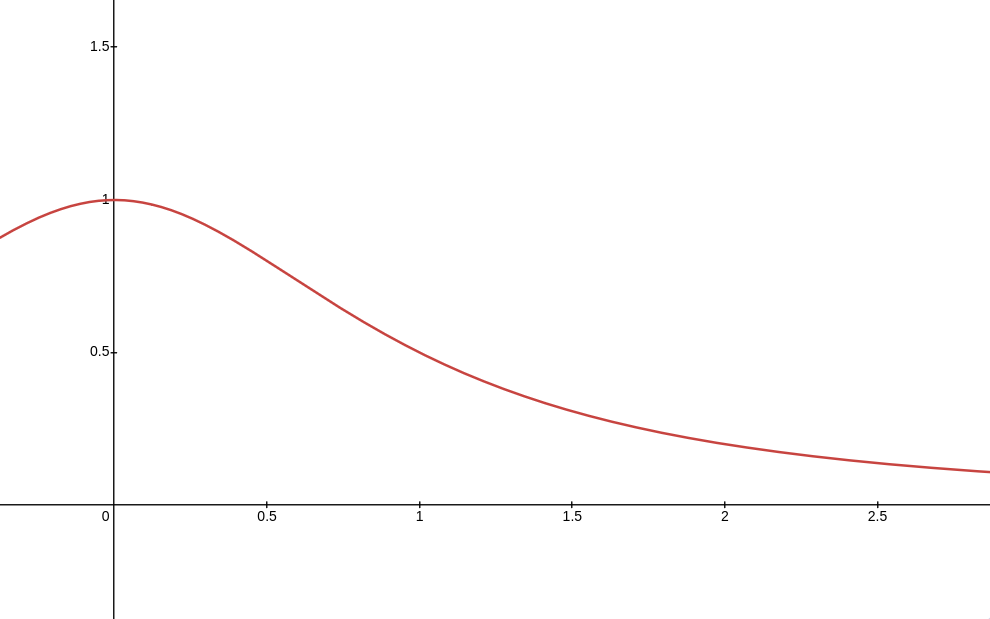
\includegraphics[width=\textwidth]{images/normalplot.png}
        \caption{Plot della funzione $f(x) = \frac{1}{x^2 + 1}$}
    \end{subfigure}
    \hfill
    \begin{subfigure}[t]{0.45\textwidth}
        \centering
        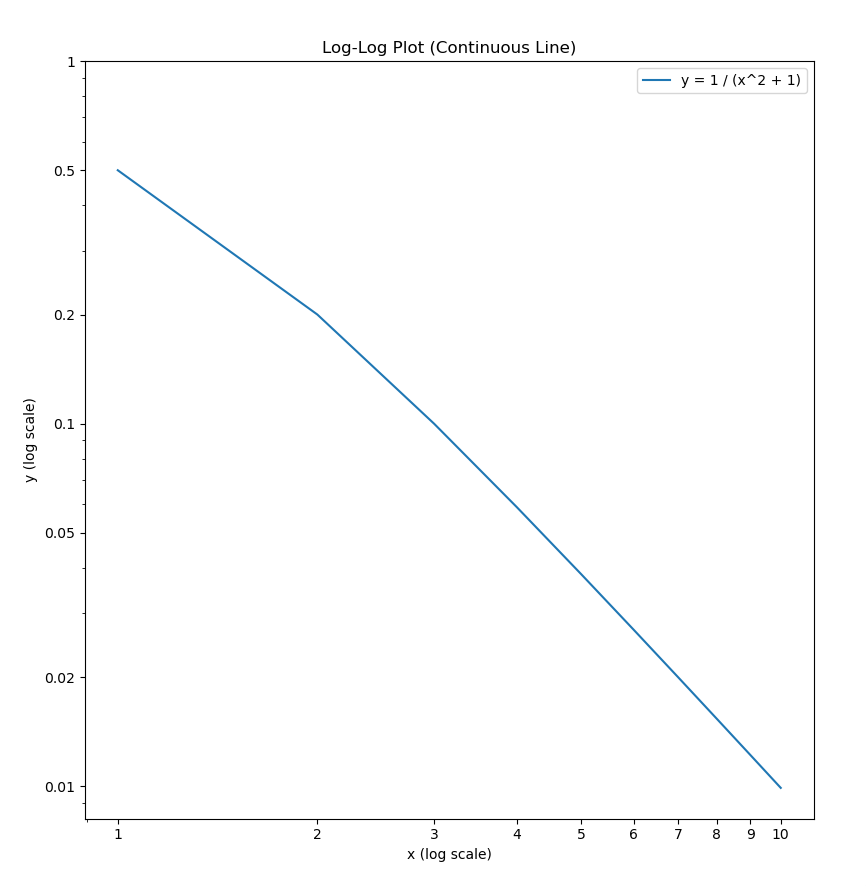
\includegraphics[width=\textwidth]{images/loglog.png}
        \caption{Plot della funzione $\ln(f(x)) = \ln\left(\frac{1}{x^2 + 1}\right)$}
    \end{subfigure}
    \label{fig:doppia}
\end{figure}

\subsection{Fenomeno Rich Get Richer}

 Il fenomeno "rich get richer" descrive una dinamica in cui chi ha già molte risorse o connessioni tende ad accumularne ancora di più, mentre chi parte svantaggiato resta indietro. Un esempio concreto si trova nella costruzione del grafo del web: quando crei una nuova pagina su un argomento, spesso inserisci un hyperlink verso una fonte autorevole trovata tramite motore di ricerca. La pagina che scegli di linkare è in cima ai risultati proprio perché ha già molti link entranti, quindi è considerata più autorevole. Così, aggiungendo il tuo link, contribuisci ad aumentare ulteriormente il grado di quella pagina già popolare. \textbf{In pratica, scegliamo quale arco aggiungere sulla base degli archi già presenti!}

\subsection{Modello Barabasi-Albert}

A questo punto vogliamo definire un modello di generazione di grafi aleatori che esprima il fenomeno "rich get richer", nel quale l'aggiunta di un nuovo arco dipenda dagli archi già presenti nel grafo, e che tale modello esibisca una power law.
\vspace{0.5cm}
\begin{definizione}[Modello Barabasi-Albert]
    Fissato $p \in [0, 1]$. Definiamo il grafo diretto $G_{p} = \{V_{p}, E_{p}\}$, il grafo aleatorio costruito nel seguente modo:
    \begin{enumerate}
        \item Al passo 1 viene creato il nodo 1: $V_{p,1} = \{1\}$;
        \item Al passo 2 viene creato il nodo 2: $V_{p,2} = \{1, 2\}$ e $E_{p,2} = \{(2, 1)\}$
        \item Al passo $i$, viene aggiunto il nodo $i$ al grafo: $V_{p,i} = V_{p, i-1} \cup \{i\}$. Successivamente, si seleziona un nodo $a$ tra quelli già presenti, scegliendolo in modo uniforme con probabilità $\frac{1}{i - 1}$. Con probabilità $p$, si aggiunge l'arco $(i, a)$ agli archi del grafo: $E_{p,i} = E_{p, i-1} \cup \{(i, a)\}$. In alternativa, con probabilità $1-p$, si aggiunge l'arco $(i, b)$, dove $b$ è il nodo destinazione dell'arco uscente da $a$: $E_{p,i} = E_{p, i-1} \cup \{(i, b)\}$.
    \end{enumerate}
\end{definizione}

 Il passo iterativo del processo di costruzione del grafo può essere anche descritto in un altro modo, al fine di formalizzare il modello.

 Al passo $i$, viene aggiunto il nodo $i$ al grafo: $V_{p,i} = V_{p, i-1} \cup \{i\}$. Con probabilità $p$, si seleziona un nodo $a$ tra quelli già presenti in modo uniforme con probabilità $\frac{1}{i - 1}$ e si aggiunge l'arco $(i, a)$ agli archi del grafo: $E_{p,i} = E_{p, i-1} \cup \{(i, a)\}$. In alternativa, con probabilità $1-p$, si seleziona un nodo $a$ tra quelli già presenti in modo uniforme con probabilità $\frac{1}{i - 1}$ e si aggiunge l'arco $(i, b)$, dove $b$ è il nodo destinazione dell'arco uscente da $a$: $E_{p,i} = E_{p, i-1} \cup \{(i, b)\}$.

\vspace{0.5cm}

 È facile conviversi che le due descrizioni sottintendono lo stesso modello di grafo. Abbiamo dunque definito un modello che descrive il fenomeno \textbf{Rich Get Richer}. Rimane da verificare se i grafi generati in accordo a questo modello esibiscono una Power Law, ossia che la funzione che descrive il numero atteso di nodi di grado $k$ si comporta come l'inverso di un polinomio.

\vspace{0.5cm}


 \subsubsection{Formalizzazione del modello}

Iniziamo con formalizzare il modello di Barabasi Albert. Come primo risultato, vogliamo definire qual è la probabilità che un arco $(i,j) \in E_{p}$. Formalmente, $\forall (i,j): i > j$ con $i \geq 2$, definiamo la variabile aleatoria
\[
    d_{ij} = 
\begin{cases}
    1 \text{ se }(i,j) \in E_p \\
    0 \text{ altrimenti}
\end{cases}
\]

 In base alle regole definite al passo iterativo, abbiamo che:
\begin{align*}
    \Pr[d_{ij} = 1] &= p \cdot \text{probabilità che venga scelto il nodo } j  \\ 
    &+ (1 - p) \cdot \text{probabilità che venga scelto un nodo } h \text{ tale che } d_{hj} = 1 \\
    &= \frac{p}{i - 1} + (1 - p) \Pr[\bigcup_{h < i:\ (h, j) \in E_p} (\text{viene scelto } h)] \\
    &= \frac{p}{i - 1} + (1 - p) \sum_{h = 1:\ (h, j) \in E_p}^{i-1} \Pr[\text{viene scelto } h] \\
    \intertext{Poiché gli eventi sono disgiunti, l'unione degli eventi è uguale alla somma delle probabilità.}
    &= \frac{p}{i - 1} + (1 - p) \sum_{h = 1:\ (h, j) \in E_p}^{i-1} \frac{1}{i - 1} \\
    &= \frac{p}{i - 1} + \frac{1 - p}{i - 1} \sum_{h = 1:\ (h, j) \in E_p}^{i-1} 1 \\
    &= \frac{p}{i - 1} + \frac{1 - p}{i - 1} \sum_{h = 1}^{i-1} d_{hj}
\end{align*}

Quindi la probabilità che ci sia l'arco $(i,j)$ è:
\[
\Pr[(i,j) \in E_p] = \Pr[d_{ij} = 1] = \frac{p}{i - 1} + \frac{1 - p}{i - 1} \sum_{h = 1}^{i-1} d_{hj}
\]

\begin{osservazione}
    Notiamo che nella definizione della variabile aleatoria $d_{ij}$, $i \geq 2$, infatti, ha senso calcolare $\Pr[(i,j)\in E_p]$ solo per $i \geq 2$ in quanto il nodo 1 non ha archi uscenti. 
\end{osservazione}

\begin{osservazione}
    Ogni nodo $i > 1$ ha esattamente un arco uscente. Quindi, per forza di cose, deve essere che
    \[
    \Pr[\exists\ j < i:\ (i,j) \in E_p] = 1
    \]
    In altre parole: per ogni nodo $i > 1$, per costruzione del grafo, esiste con certezza un nodo $j < i$ tale che $(i, j) \in E_p$.
\end{osservazione}

\begin{proof}[Per induzione]
    \[
    \Pr[\exists\ j < i:\ (i,j) \in E_p] = \sum_{j = 1}^{i-1} \Pr[(i,j) \in E_p]
    \]
    \begin{itemize}
        \item {\textbf{[Caso Base]} $i = 2$:
        \[
            \sum_{j = 1}^1 \Pr[(2,j) \in E_p] = \Pr[(2,1) \in E_p] = 1 \text{ per costruzione}
        \]
        }
        \item {\textbf{[Passo Induttivo]}: Assumiamo che $\sum_{1 \leq j<a} \Pr[(a,j) \in E_p ] = 1\ \forall\ a \leq i - 1$}, si ha che
        \begin{align*}  
        \sum_{j = 1}^{i - 1} \Pr[(i,j) \in E_p] &= \sum_{j = 1}^{i-1}\left( \frac{p}{i-1} + \frac{1-p}{i-1} \sum_{h=1}^{i-1} d_{hj} \right) \\
        &= \sum_{j = 1}^{i-1} \frac{p}{i-1} + \sum_{j=1}^{i-1} \frac{1-p}{i-1} \sum_{h=1}^{i-1} d_{hj} \\ 
        &= \frac{(i-1)p}{i-1} + \frac{1-p}{i-1} \sum_{h=1}^{i-1} \sum_{j=1}^{i-1} d_{hj} \\
        \intertext{Per ipotesi ind., ogni $h < i$ ha esattamente un arco uscente e quindi, $\sum_{1 \leq h < i} d_{hj} = 1$} \\
        &= p + \frac{1 - p}{i - 1} \sum_{h = 1}^{i-1} 1 = p + (1 - p) = 1
        \end{align*}
    \end{itemize}
\end{proof}

\begin{osservazione}[Interpretazione regola iterativa]
    Data la formula 
    \[
    \Pr[(i,j) \in E_p] = \frac{p}{i - 1} + \frac{1 - p}{i - 1} \sum_{h = 1}^{i-1} d_{hj}
    \]
    possiamo, interpretare la regola iterativa con la quale viene generato il grafo nel seguente modo: 
    Il nodo $j$ a cui connettere $i$ è scelto
\begin{itemize}
    \item \textbf{uniformemente a caso con probabilità} $p$
    \[
    \frac{p}{i-1}
    \]
    \item \textbf{con probabilità proporzionale al grado} $j$ con probabilità $1-p$
    \[
    \frac{1-p}{i-1}\sum_{h=1}^{i-1}d_{hj}
    \]
\end{itemize}
 In questo modo, la regola esprime chiaramente il fenomeno \textbf{Rich get Richer}.
\end{osservazione}

Rimane da dimostrare che il modello di Barabasi-Albert, oltre a esprimere il fenomeno Rich get Richer, esibisce anche una \textbf{Power Law}. La dimostrazione consiste di 4 punti:
\begin{enumerate}
    \item Definizione della legge aleatoria che esprime la variazione del grado di un nodo nel tempo. [\autoref{sec:legge}]
    \item Approssimazione deterministica e continua della legge al punto 1, che porterà ad una equazione \textbf{differenziale}. [\autoref{sec:approssimazione}]
    \item Risoluzione dell'equazione differenziale: la soluzione costituirà un'approssimazione della funzione che esprime il grado di un nodo nel tempo. [\autoref{sec:risoluzione}]
    \item Individuazione della Power Law. [\autoref{sec:powerlaw}]
\end{enumerate}

\newpage

\subsubsection{Legge aleatoria per la variazione del grado}\label{sec:legge}
\vspace{0.5cm}

\begin{definizione}[Legge aleatoria]
    Definiamo $D_j(t)$ la variabile aleatoria che esprime il numero di archi entranti nel nodo $j$ al passo $t$ di generazione del grafo, dove $t \geq j,\ \forall\ j \geq 1$.
    Al passo $t=j$, il grado entrante di $j$ è 0, in quanto al passo $j$ il nodo è appena stato creato (passo iterativo dell'algoritmo di generazione). 
    \[
    D_j(j) = 0
    \]
    ciò esprime la condizione iniziale della variabile.
    Analizziamo ora la variazione attesa nel tempo della variabile $D_j(t)$. Al passo $t+1$, il grado di $j$ può essere invariato rispetto al passo $t$ (se $j$ non viene scelto al passo iterativo) oppure può essere aumentato di un'unità, ovvero
    \[
    D_j(t+1) = D_j(t) + 1 \iff \text{ è stato creato l'arco } (t+1, j)
    \]
    dunque,
    \[
    \Pr[D_j(t+1) - D_j(t) = 1] = \Pr[d_{t+1j} = 1] = \frac{p}{t} + \frac{1-p}{t}\sum_{h=1}^t d_hj = \frac{p}{t} + \frac{1-p}{t} D_j(t)
    \]
    In conclusione, abbiamo definito come varia il numero di archi entranti nel nodo $j$ al passo $t+1$.
    \[
    \Pr[D_j(t+1) - D_j(t) = 1] = \frac{p}{t} + \frac{1-p}{t} D_j(t)
    \]
    \[
    D_j(j) = 0 \text{ condizione iniziale}
    \]
\end{definizione}

\subsubsection{Approssimazione deterministica e continua}\label{sec:approssimazione}
\vspace{0.5cm}

Adesso dobbiamo trovare una funzione deterministica continua che ci permette di approssimare la legge aleatoria trovata prima. Iniziamo con definire una funzione \textit{deterministica discreta}.

\begin{definizione}[Funzione deterministica discreta]
    $\forall j \geq 1 \text{ e } \forall t \geq j$ definiamo $X_j(t)$ nel seguente modo:
    \begin{itemize}
        \item $X_j(j) = 0$
        \item $X_j(t+1) - X_j(t) = \frac{p}{t} + \frac{1-p}{t}X_j(t)$
    \end{itemize}
\end{definizione}

 Approssimiamo ora la funzione discreta definita sopra con una funzione \textit{continua}.

\begin{definizione}[Funzione deterministica continua]
    Definiamo la funzione $x_j(t)$ definita su un dominio continuo, con $t \geq j$, nel seguente modo:
    \begin{itemize}
        \item $x_j(j) = 0$
        \item $\frac{d}{dt}x_j(t) = \frac{p}{t} + \frac{1-p}{t}x_j(t)$
    \end{itemize}
    ottenendo un'equazione differenziale. Non è detto che l'andamento della funzione $x_j(t)$ sia effettivamente vicino al comportamento della variabile aleatoria $D_j(t)$, ma le analogie fra le due sono forti.
\end{definizione}

\newpage

\subsubsection{Risoluzione dell'equazione differenziale}\label{sec:risoluzione}
\vspace{0.5cm}

 Ora ci occuperemo di risolvere l'equazione differenziale
\begin{align*}
\frac{d}{dt}x_j(t) &= \frac{p}{t} + \frac{1-p}{t}x_j(t) \\
&= \frac{1}{t}[p + (1-p)x_j(t)]
\end{align*}
Da cui segue
\[
\frac{1}{p+(1-p)x_j(t)} \frac{d\ x_j(t)}{dt} = \frac{1}{t}
\]
Integrando poi ambo i membri, otteniamo:
\begin{align*}
&\quad\quad\quad \int \frac{1}{p+(1-p)x_j(t)} \frac{d\ x_j(t)}{dt} dt = \int \frac{1}{t}dt\\
&\iff
\int \frac{d\ x_j(t)}{p+(1-p)x_j(t)} = \int \frac{1}{t}dt \\
&\iff
\int \frac{(1-p)d\ x_j(t)}{p+(1-p)x_j(t)} = (1-p)\int \frac{1}{t}dt \\
\intertext{Sostituiamo $y = p+(1-p)x_j(t)$, in quanto il numeratore è la derivata del denominatore, ottenendo $dy = (1-p)dx_j(t)$}
&\iff \int \frac{dy}{y} = (1-p)\int \frac{1}{t}dt
\intertext{Integrando, otteniamo}
&\iff \ln[p + (1 - p)x_j(t)] = (1-p)\ln(t) + c = \ln(t^{1-p}) + c
\intertext{Esponenziando, otteniamo}
&\iff p + (1-p)x_j(t) = t^{1-p}e^c
\intertext{Imponiamo $H = e^c$ una costante positiva, e per trovarla, si impone la condizione iniziale, $x_j(j) = 0$}
&\iff p = H j^{1-p} \iff H = \frac{p}{j^{1-p}}
\end{align*}
In conclusione, otteniamo che
\[
x_j(t) = \frac{p}{1-p}\left[ \left(\frac{1}{j}\right)^{1-p} - 1\right]
\]

\newpage

\subsubsection{Individuazione della Power Law}\label{sec:powerlaw}
\vspace{0.5cm}

 Rimane ora da calcolare nel modello deterministico continuo, dati $k$ e $t$, la frazione dei nodi, che al passo $t$, ha grado $k$. Sapendo che, al passo $t$ l'insieme dei nodi è $[t] = \{1, 2, 3, \dots, t\}$, definiamo l'insieme:
\[
A_t(k) = \{j \leq t:\ x_j(t) \geq k\}
\]
ovvero l'insieme dei nodi con grado almeno $k$.
A noi interessa la \textbf{frazione} dei nodi di grado\textbf{esattamente} $k$, dunque vogliamo calcolare
\[
\frac{1}{t}|A_t(k) - A_t(k + 1)| = \frac{1}{t}[|A_t(k)| - |A_t(k+1)|]
\]
vale l'uguaglianza in quanto $A_t(k + 1) \subseteq A_t(k)$.
\begin{figure}[ht!]
    \centering
        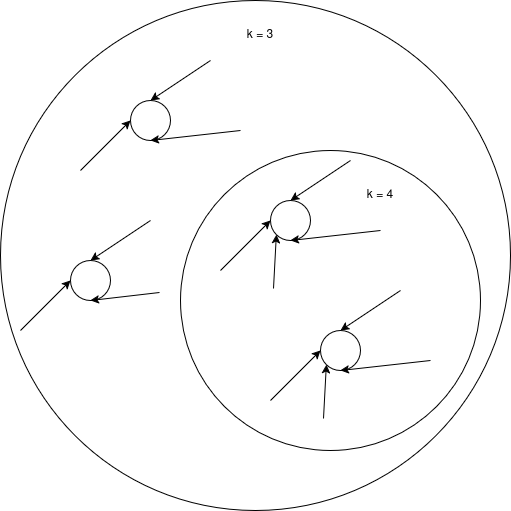
\includegraphics[width=0.5\textwidth]{images/powerLaw.png}
        \caption{$A_t(k + 1) \subseteq A_t(k)$}
\end{figure}

 Per definizione, il nodo $j \in A_t(k) \iff j \leq t\ \land\ x_j(t) \geq k$. Espandendo la seconda condizione, abbiamo che:
\begin{align*}
x_j(t) &= \frac{p}{1-p}\left[\left( \frac{1}{j}\right)^{1-p} - 1\right] \geq k \\
&\iff \left( \frac{1}{j}\right)^{1-p} \geq \frac{1-p}{p}k + 1 \\
&\iff \left( \frac{1}{j}\right) \geq \left[\frac{1-p}{p}k + 1\right]^{\frac{1}{1-p}} \\
&\iff j \leq t\left[\frac{1-p}{p}k + 1\right]^{-\frac{1}{1-p}}
\end{align*}
Osserviamo adesso che 
\[
\left.
\begin{aligned}
& \frac{1-p}{p}k + 1 > 1 \\
& -\frac{1}{1-p} < 0
\end{aligned}
\right\}
\;\Rightarrow\;
\left[\frac{1-p}{p}k + 1\right]^{-\frac{1}{1-p}} < 1
\;\Rightarrow\; t\left[\frac{1-p}{p}k + 1\right]^{-\frac{1}{1-p}} < t
\]
In conclusione, 
\[
A_t(k) = \left\{j\ |\ j \leq t\left[\frac{1-p}{p}k + 1\right]^{-\frac{1}{1-p}}\right\}
\]
quindi,
\[
|A_t(k)| = t\left[\frac{1-p}{p}k + 1\right]^{-\frac{1}{1-p}}
\]
Riuscendo quindi a calcolare la dimensione dell'insieme $A_t(k)$. Con questo risultato, possiamo adesso calcolare quanto vale la frazione dei nodi con grado esattamente $k$ (il numero di nodi con grado almeno $k$ - il numero di nodi con grado almeno $k + 1$), ovvero:
\[
\frac{1}{t}[|A_t(k)| - |A_t(k+1)|]
\]
Per semplicità, definiamo:
\[
F(k) = \left[\frac{1-p}{p}k + 1\right]^{-\frac{1}{1-p}}
\]
ottenendo quindi,
\[
f(k) = F(k) - F(k + 1) = \frac{1}{t}[|A_t(k)| - |A_t(k+1)|]
\]
Poiché $f(k) = F(k) - F(k + 1)$, possiamo approssimarla con la sua derivata, ovvero, $f(k) \approx - \frac{dF(k)}{dk}$, quindi:
\[
\begin{aligned}
f(k) \approx - \frac{dF(k)}{dk} &= \frac{(1-p)}{p}\left[-\frac{1}{1-p}\right]\left[\frac{(1-p)}{p}k+1\right]^{-\frac{1}{1-p}-1}\\
&= \frac{1}{p}\left[\frac{(1-p)}{p}k+1\right]^{-\frac{1}{1-p}-1} 
\end{aligned}
\]
Che è una \textbf{Power Law} con esponente $1 + \frac{1}{1-p}$.
In conclusione, nel modello Rich Get Richer, con alta probabilità la frazione del numero di nodi di grado $k$ è proporzionale a 
\[k^{-\frac{1}{1-p}-1}.\]

\newpage

\section{Grafi Geometrici aleatori e reti wireless}

Fino adesso abbiamo parlato di modelli di generazione di grafi aleatori per reti virtuali. In questo capitolo ci focalizziamo invece sulle reti fisiche, nel dettaglio sulle reti wireless ad hoc.

Le reti wireless ad hoc sono composte da nodi dotati di ricetrasmettitori che comunicano in modalità peer-to-peer, spesso tramite percorsi multi-hop, cioè attraverso nodi intermedi che inoltrano i messaggi fino alla destinazione.  

Le reti di sensori rappresentano una particolare categoria di reti ad hoc, in cui ogni nodo include un sensore, una batteria a bassa capacità, un processore semplice e un modulo wireless. Questi nodi raccolgono e trasmettono dati ambientali (come temperatura o pressione), eventualmente comprimerli o aggregarli, per fornire una visione complessiva dell'area monitorata. I dati possono poi essere accessibili da utenti esterni tramite nodi gateway.  

Le applicazioni spaziano dal monitoraggio ambientale e meteorologico al controllo di infrastrutture e sistemi industriali.

Per garantire la comunicazione tra tutti i nodi di una rete, questa deve essere connessa: per ogni coppia di nodi deve esistere un percorso di collegamenti diretti (multi-hop) che permetta alle informazioni di viaggiare da uno all'altro.

\vspace{0.5cm}

\begin{definizione}[Grafo Geometrico]
    Un grafo geometrico G = \{V, E, r\} consiste in un insieme $V$ di nodi in uno spazio metrico ($\mathbb{R}^2$), dei quali conosciamo le coordinate, e un parametro $r > 0$. Quindi: 
    \begin{itemize}
        \item $V = \mathbb{R}^2$, quindi $\forall,\ A \in V,\ A = \{x_A, y_B\}$.
        \item $E = \{(A, B): A \in V \land B \in V \land \sqrt{(x_A - x_B)^2 + (y_A - y_B)^2} \leq r\}$
    \end{itemize}
\end{definizione}

Generalmente si normalizza per $r$, ossia si riportano i punti in scala $1:r$. In questo caso, quando $r = 1$, il grafo prende il nome di \textbf{Unit Disk Graph}.

\vspace{0.5cm}

\begin{definizione}[Grafo Geometrico Aleatorio]
    Siano $n \in \mathbb{N}$ e $0 < r \leq \sqrt{2}$. Un \textbf{grafo geometrico aleatorio} $G(n, r)$ è un particolare grafo geometrico, definito all'interno di un quadrato $Q = [0,1] \times [0, 1]$. In pratica vengono scelti uniformemente a random $n$ punti all'interno di $Q$.
\end{definizione}

La scelta che $0 < r \leq \sqrt{2}$ dipende appunto dal fatto che $Q$ è il quadrato unitario, la cui diagonale misura $\sqrt{2}$. Infatti:
\begin{itemize}
    \item $r = \sqrt{2}$, $G(n, \sqrt{2})$ è un grafo completo;
    \item $r = 0$, $G(n, 0)$ è un grafo costituito da soli nodi isolati.
    \item In generale, se $r \rightarrow 0$, il grafo diventa sempre più sparso, mentre se $r \rightarrow \sqrt{2}$, il grafo diventa sempre più completo.
\end{itemize}

Questo particolare modello può avere numerosi riscontri pratici.
Per esempio consideriamo una situazione in cui si hanno a disposizione $n$ sensori ambientali per l'acquisizione di dati utili allo studio di fenomeni atmosferici, e di doverli disporre in una vasta area di $10,\ km^2$. 
Prima di spargere i sensori è possibile impostare un raggio 
$r$ di trasmissione, utile ai sensori per scambiarsi informazioni. Ovviamente maggiore è il raggio di trasmissione  $r$, maggiore sarà il consumo di batteria dei sensori.
Questi sensori inoltre verranno rilasciati nell'ambiente in maniera casuale lanciandoli da un aereo che sorvolerà l'area.

L'obiettivo è ora trovare il più piccolo valore di $r = r(n)$ (in funzione di $n$) tale che, con buona probabilità, la rete $G(n, r(n))$ risulti sempre connessa al crescere di $n$.

\subsection{Reti Wireless ad-hoc}

Per contestualizzare meglio il problema che stiamo studiando, consideriamo le \textbf{reti wireless ad-hoc}.

Una rete wireless ad-hoc è costituita da un insieme di dispositivi, ad esempio calcolatori o sensori, dislocati in un area. Ciascun dispositivo è dotato di un ricetrasmettitore wireless e di una batteria di capacità limita.

Ciascun ricetrasmettitore può essere configurato affinché possa trasmettere entro un certo raggio, che prende il nome di raggio di trasmissione.
\begin{definizione}[Raggio di trasmissione]
    Il raggio di trasmissione $r_x$ di un trasmettitore $x$ è la distanza entro la quale il dispositivo può inviare/riceve messaggi.    
\end{definizione}

\vspace{0.5cm}

\begin{definizione}[Grafo di comunicazione]
    Ad una rete di comunicazione è associato un grafo diretto, chiamato grafo di comunicazione. I nodi di questo grafo sono sono i dispositivi della rete. Dati due dispositivi $x$ e $y$, allora esiste l'arco $(x, y) \iff d(x, y) \leq r_x$.
\end{definizione}

\begin{figure}[ht!]
    \centering
    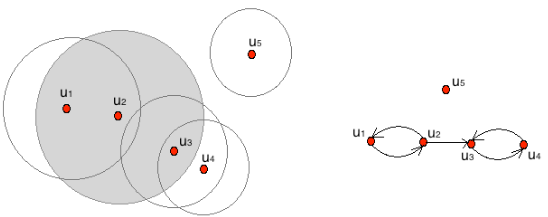
\includegraphics[width=0.5\linewidth]{images/grafo_comunicazione.png}
    \caption{Grafo di comunicazione}
    \label{fig:gc}
\end{figure}

Quindi, quando un nodo proverà a trasmettere ad un nodo che non rientra nel suo raggio di trasmissione, non potrà inviarlo direttamente ma dovrà utilizzare un percorso all'interno del grafo. Una comunicazione di questo tipo prende il nome di \textbf{comunicazione multi-hop}. Infatti, nella \autoref{fig:gc}, $u_1$ può inviare un messaggio a $u_4$ utilizzando il percorso $\{(u_1, u_2), (u_2, u_3),(u_3, u_4)\}$. Ovviamente, un nodo $x$ può inviare messaggi ad un nodo $y$ solo se esiste un percorso $x, \dots, y$ all'interno del grafo. 

 Perciò, se vogliamo che ciascun nodo possa comunicare con qualunque altro nodo è necessario che il grafo di comunicazione sia \textbf{fortemente connesso}. Questo problema si può risolvere facilmente impostando a ciascun nodo il raggio di trasmissione pari alla distanza di quel nodo dal nodo ad esso più distante, ovvero:

 Sia $V$ l'insieme dei nodi e sia $d(u, v)$ la distanza tra $u$ e $v$, allora,
\[
\forall\ u \in V,\ r_u = \max\{d(u, v):\ v \in V - \{u\}\}
\]

In questo modo, ciascun nodo può comunicare con qualunque altro nodo. Il problema è che l'energia che occorre ad un nodo per trasmettere i suoi messaggi è tanto maggiore quanto è più grande il raggio di trasmissione di quel nodo, perciò dobbiamo assegnare a ciascun nodo un raggio di trasmissione più piccolo.

 Riassumendo, possiamo modellare il problema descritto sopra nel seguente modo.
Assumiamo che tutti gli $n$ nodi abbiano lo stesso raggio di trasmissione $r(n)$. Inoltre, assumiamo che gli $n$ nodi siano distribuiti uniformemente a caso in un quadrato $Q = [0,1] \times [0, 1]$. La rete dunque è modellata da un grafo geometrico aleatorio $G(n, r(n))$, non orientato, in quanto $d(x, y) \leq r(n) \iff d(y, x) \leq r(n)$.

Il problema che dobbiamo studiare è:
\textbf{Dati $n$ punti distribuiti uniformemente a caso nel quadrato $Q = [0, 1] \times [0, 1]$ calcolare il valore minimo di $r(n)$ affinché $G(n, r(n))$ sia connesso}.

\subsection{Connessione di $G(n, r(n))$}

In questa sezione ci occuperemo di dimostrare la connettività di $G(n, r(n))$.

\begin{teorema}[Connessione di $G(n, r(n))$]
    Sia $r^*(n) = \min\{r(n)\}$ che garantisce, con probabilità ragionevole, che $G(n, r(n))$ è connesso, allora,
    \[
    r^*(n) \in \Theta\left(\sqrt{\frac{\ln n}{n}}\right)
    \]
\end{teorema}

Per mostrare la precedente affermazione è necessario dimostrare due teoremi che mostrano rispettivamente una \textbf{limitazione superiore ed una inferiore} per il minimo raggio di trasmissione $r^*(n)$.

\subsubsection{Delimitazione superiore al minimo raggio di connessione}

 \begin{teorema}[Delimitazione superiore al minimo raggio di connessione]
    Esiste una costante $\gamma_1 > 0$ tale che se $r(n) \geq \gamma_1 \left(\sqrt{\frac{\ln n}{n}}\right)$, allora $G(n, r(n))$ è connesso con \textbf{alta probabilità}.
\end{teorema}

\begin{proof}
    Sia $k(n) > 0$ un intero (dipendente da $n$). Partizioniamo $Q = [0, 1] \times [0, 1]$ in $k^2(n)$ celle, ciascuna di lato $\frac{1}{k(n)}$. Poniamo $r(n)$ pari alla lunghezza della diagonale di una coppia di celle adiacenti (due celle aventi un lato in comune), ovvero
    \[
    r(n) = \sqrt{\left(\frac{2}{k(n)}\right)^2 + \left(\frac{2}{k(n)}\right)^2} = \frac{\sqrt{5}}{k(n)}
    \]

\begin{figure}[ht!]
    \centering
    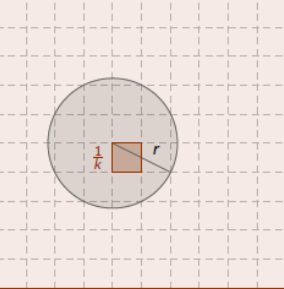
\includegraphics[width=0.3\linewidth]{images/delsup1.png}
    \label{fig:placeholder}
\end{figure}

 Ponendo $r(n) = \frac{\sqrt{5}}{k(n)}$, ciascun nodo in una qualsiasi cella è collegato da un arco a \textbf{tutti} i nodi (eventualmente) contenuti in tutte le celle adiacenti. Quindi se riuscissimo a dimostrare che con alta probabilità ciascuna cella contiene \textbf{almeno} un nodo, avremmo dimostrato che $G(n, r(n))$ è connesso con alta probabilità.

 \textbf{Dobbiamo quindi dimostrare che è possibile scegliere $k(n)$ in modo tale che, con alta probabilità, nessuna cella è vuota}.
Per calcolare questa probabilità, per semplicità consideriamo la probabilità complementare, ovvero che \textbf{esiste almeno una cella vuota}.

 Sia $C$ una cella, l'obbiettivo è trovare una \textbf{delimitazione superiore} alla probabilità che 
\[\Pr[C = \emptyset]\]
L'evento $C = \emptyset$ lo possiamo scrivere come intersezione di più eventi, ovvero
\[
C = \emptyset \iff 1 \notin C \land 2 \notin C \land \dots \land n \notin C = \bigcap_{1 \leq i \leq n}(i \notin C)
\]
Da cui segue
\[
\Pr[C = \emptyset] = \Pr\left[\bigcap_{1 \leq i \leq n}(i \notin C)\right]
\]
Poiché i nodi sono posizionati in $Q$ \textbf{indipendentemente} gli uni dagli altri
\[
\Pr\left[\bigcap_{1 \leq i \leq n}(i \notin C)\right] = \prod_{1 \leq i \leq n}\Pr(i \notin C)
\]
Dobbiamo ora capire quanto vale $\Pr(i \notin C) = 1 - \Pr(i \in C)$. La probabilità che il nodo $i$ sia scelto all'interno della cella $C$ è pari al rapporto fra l'area di $C$ e l'area del quadrato $Q = [0,1] \times [0,1]$. Quindi
\[
\Pr[i \in C] = \frac{Area_C}{Area_Q} = \frac{1}{k^2(n)}
\]
Da cui segue che
\[
\Pr(i \notin C) = 1 - \Pr(i \in C) = 1 - \frac{1}{k^2(n)}
\]
Quindi
\[
\Pr[C = \emptyset] = \Pr\left[\bigcap_{1 \leq i \leq n}(i \notin C)\right] = \prod_{1 \leq i \leq n}\Pr(i \notin C) = \left(1 - \frac{1}{k^2(n)}\right)^n
\]
Calcolata la probabilità che la cella $C$ sia vuota, si vuole ora calcolare la probabilità dell'evento che esista \textbf{almeno} una cella vuota, ovvero
\[
\Pr[\exists\ C: C = \emptyset] = \Pr\left[\bigcup_{C \in Q}(C = \emptyset)\right]
\]
Applicando la Union Bound\footnote{La Union Bound dice che la probabilità dell'unione di eventi è minore o uguale della somma delle loro probabilità}
\[
\Pr[\exists\ C: C = \emptyset] \leq \sum_{C \in Q}\Pr[C = \emptyset] \leq k^2(n)\left(1 - \frac{1}{k^2(n)}\right)^n
\]
Sostituendo $k(n) = \frac{\sqrt{5}}{r(n)}$, otteniamo che
\[
\Pr[\exists\ C: C = \emptyset] \leq \sum_{C \in Q}\Pr[C = \emptyset] \leq \frac{5}{r^2(n)}\left(1 - \frac{r^2(n)}{5}\right)^n
\]
A questo punto, poniamo $r(n) = \gamma_1\left(\sqrt{\frac{\ln n}{n}}\right)$ ottenendo,
\[
\Pr[\exists\ C: C = \emptyset] \leq \sum_{C \in Q}\Pr[C = \emptyset] \leq \frac{5n}{\gamma_1^2\ln n}\left(1 - \frac{\gamma_1^2\ln n}{5n}\right)^n
\]
Sapendo che $\forall x \in \mathbb{R},\ 1 - x \leq e^{-x}$ e inoltre, se $x \neq 0$, allora $1 - x < e^{-x}$.

 Poiché $\frac{\gamma_1^2\ln n}{5n} \neq 0$, per ogni $n \in \mathbb{N}$, otteniamo che
\[
\left(1 - \frac{\gamma_1^2\ln n}{5n}\right)^n < e^{-\frac{\gamma_1^2\ln n}{5n}}
\]
Quindi
\begin{align*}  
\Pr[\exists\ C: C = \emptyset] &< \frac{5n}{\gamma_1^2\ln n}e^{-\cancel{n}\frac{\gamma_1^2\ln n}{5\cancel{n}}} < \frac{5n}{\gamma_1^2}e^{-\frac{\gamma_1^2\ln n}{5}} \\
&= \frac{5n}{\gamma_1^2}n^{-\frac{\gamma_1^2}{5}} = \frac{5}{\gamma_1^2}n^{1 - \frac{\gamma_1^2}{5}}
\end{align*}
Poiché vogliamo che questa probabilità sia più piccola possibile, ovvero che
\[
\Pr[\exists\ C: C = \emptyset] < \frac{b}{n^c} \in \left(\frac{1}{n}\right)^{\Omega(1)}
\]
l'esponente $1 - \frac{\gamma_1^2}{5}$ deve essere negativo. Infatti, per $\gamma_1 > \sqrt{5},\ 1 - \frac{\gamma_1^2}{5} < 0$, quindi
con alta probabilità
\[
\Pr[G(n, r(n) \text{ è connesso })] \geq \Pr[\nexists\ C = \emptyset] = 1 - \Pr(\exists\ C: C = \emptyset) > 1 - \frac{b}{n^c} = 1 - \frac{5}{\gamma_1^2}n^{1 - \frac{\gamma_1^2}{5}} 
\]
In conclusione, abbiamo dimostrato che se $r(n) = \gamma_1\left(\sqrt{\frac{\ln n}{n}}\right)$ e $\gamma_1 > \sqrt{5}$, il grafo $G(n, r(n))$ è connesso con alta probabilità.
\end{proof}

\subsubsection{Delimitazione inferiore al minimo raggio di connessione}

\begin{osservazione}
    Nella prova della delimitazione superiore, ossia, che $r^*(n) \leq \gamma_1\left(\sqrt{\frac{\ln n}{n}}\right)$, abbiamo dovuto cercare una \textbf{maggiorazione} della probabilità che $G(n, r(n))$ è non connesso, ossia abbiamo dovuto dimostrare che $\Pr[G \text{ non connesso}] \leq \text{qualcosa}$.

     Ora, per dimostrare che $r^*(n) \geq \sqrt{\frac{\ln (n) + c}{n}}$, dobbiamo dimostrare una \textbf{minorazione} della probabilità che $G(n, r(n))$ è non connesso, ossi, dobbiamo dimostrare che $\Pr[G \text{ non connesso}] \geq \text{qualcosa}$.
\end{osservazione}

\begin{teorema}[Delimitazione inferiore al minimo raggio di connessione]
    Per ogni costatante $c > 0$, se $r(n) = \sqrt{\frac{\ln(n) + c}{n \pi}}$, allora 
    \[\lim_{n \rightarrow \infty} \Pr[G(n, r(n) \text{ è non connesso }] > 0
    \]
\end{teorema}

\begin{proof}
    Nel corso della dimostrazione, denoteremo con $G = G(n, r(n))$ e con $r = r(n)$. Come anticipato prima, dobbiamo trovare una \textbf{minorazione} per $\Pr[G \text{ non connesso}]$. Per iniziare, introduciamo i seguenti eventi:
    \begin{itemize}
        \item $\mathcal{E}_{\geq 1} = G$ contiene \textbf{almeno} un nodo isolato.
        \item $\mathcal{E}_{i_1, i_2, \dots, i_h} = $ tutti i nodi $i_1, i_2, \dots, i_h$ sono isolati in $G$, con $i_1, i_2, \dots, i_h \in [n]$.
        \item $\mathcal{E}_{i!} = i$ è l'unico nodo isolato in $G$, con $i \in [n]$.
    \end{itemize}

 Ai fini della dimostrazione, dobbiamo ricordare la seguente proposizione: 
 Dati due eventi $A$ e $B$, se $A \implies B$, allora
\[
    \Pr[A] \leq \Pr[B].    
\]

 Questo significa che ogni volta che accade $A$ accade anche $B$ (in termini insiemistici $A \subseteq B$). 
Ora, la probabilità è una \textbf{misura} (nel senso matematico): più grande è l'insieme, più grande (o uguale) è la sua probabilità, quindi
\begin{align}
A \subseteq B \implies \Pr[A] \leq \Pr[B]
\end{align}

 Ritornando alla nostra dimostrazione, possiamo fare le seguenti osservazione:
\begin{itemize}
    \item {
        se $G$ contiene almeno un nodo isolato allora $G$ è non connesso, ovvero
        \[
        \mathcal{E}_{\geq 1} \implies \text{G non connesso}
        \]
        Implica
        \[
        \Pr[\mathcal{E}_{\geq 1}] \leq \Pr[\text{G non connesso}]
        \]
    }
    \item {
        Inoltre, se accade che 1 è l'unico nodo isolato in $G$, oppure 2 è l'unico nodo isolato in $G$, oppure $\dots$, oppure $n$ è l'unico nodo isolato in $G$, allora accade che $G$ contiene un nodo isolato, formalmente, se
        \[
        \bigcup_{i \in [n]} \mathcal{E}_{i!} \implies \mathcal{E}_{\geq1}
        \]
        allora
        \[
        \Pr\left[\bigcup_{i \in [n]} \mathcal{E}_{i!}\right] \leq \Pr[\mathcal{E}_{\geq1}]
        \]
    }
\end{itemize}

In entrambi i casi, è stata applicata la $(1)$.

Poiché $\mathcal{E}_{1!}, \mathcal{E}_{2!}, \dots, \mathcal{E}_{n!}$ sono eventi disgiunti, allora
\[
\Pr\left[\bigcup_{i \in [n]} \mathcal{E}_{i!}\right] = \sum_{i \in [n]}\Pr[\mathcal{E}_{i!}]
\]

In conclusione, abbiamo trovato una \textbf{minorazione} per $\Pr[G \text{ non connesso}]$, ovvero
\[
\Pr[G \text{ non connesso}] \geq \sum_{i \in [n]}\Pr[\mathcal{E}_{i!}]
\]

 Non è, però, semplice calcolare direttamente $\Pr[\mathcal{E}_{i!}]$. Allora, dobbiamo trovare delle espressioni più facili per poterla minorare. Osserviamo che il nodo $i$ è l'unico isolato in $G$, se e solo se $i$ è un nodo isolato in $G$ e inoltre, comunque scegliamo un altro nodo $j$, $i$ e $j$ non sono entrambi isolati in $G$, ovvero
\[
\mathcal{E}_{i1} = \mathcal{E}_i \bigcap_{j \in [n] - \{i\}} \mathcal{E}_{ij}^C = \mathcal{E}_i - \bigcup_{j \in [n] - \{i\}}\mathcal{E}_{ij}
\]
Quindi,
\begin{align*}
    \Pr[\mathcal{E}_{i!}] 
    &= \Pr\!\left[\mathcal{E}_i \setminus 
        \bigcup_{j \in [n] \setminus \{i\}}\mathcal{E}_{ij}\right] \\[4pt]
    &\underbrace{\geq}_{(1)} 
        \Pr[\mathcal{E}_i] 
        - \Pr\!\left[\bigcup_{j \in [n] \setminus \{i\}}\mathcal{E}_{ij}\right] \\[6pt]
    &\underbrace{\geq}_{(2)} 
        \Pr[\mathcal{E}_i] 
        - \sum_{j \in [n] \setminus \{i\}}\Pr[\mathcal{E}_{ij}]
\end{align*}

\smallskip

\textbf{(1)} Disuguaglianza di sottrazione per insiemi: 
\[
P(A\setminus B) = P(A) - P(A\cap B) \ge P(A) - P(B)
\]
poiché \(P(A\cap B) \le P(B)\). \\[4pt]
\textbf{(2)} Union Bound (o disuguaglianza dell'unione): 
\[
P\!\left(\bigcup_i A_i\right) \le \sum_i P(A_i)
\]

 Ricapitolando, l'obbiettivo della dimostrazione è quindi calcolare una \textbf{minorazione} per $\Pr[G \text{ non connesso}]$. Fino adesso siamo arrivati ai seguenti risultati:
\begin{enumerate}
    \item $\Pr[G \text{ non connesso}] \geq \sum\limits_{i \in [n]}\Pr[\mathcal{E}_{i!}]$
    \item $\Pr[\mathcal{E}_{i!}] \geq \Pr[\mathcal{E}_i] - \sum\limits_{j \in [n] \setminus \{i\}} \Pr[\mathcal{E}_{ij}]$
\end{enumerate}

 A questo punto non ci resta che trovare \textbf{una minorazione per $\Pr[\mathcal{E}_i]$ e una maggiorazione per $\Pr[\mathcal{E}_{ij}]$}.

Prima di procedere, indichiamo per ogni $t \in Q$, $C_r{t}$ il cerchio di centro $t$ e raggio $r$. Inoltre, per ogni $i \in [n],\ t_i \in Q$ è il punto del quadrato nel quale è posizionato il nodo $i$ (in pratica dobbiamo distinguere fra il concetto astratto di nodo e la sua posizione fisica nel piano). 

\textbf{Minoriamo $\Pr[\mathcal{E}_i]$}. L'evento $\mathcal{E}_i$ si verifica se e solo se, una volta fissato $t_i$, nessun nodo $j \neq i$ è posizionato in $C_r(t_i)$.

Quindi, \textbf{fissato} $t_i$ e \textbf{fissato} $j \neq i$,
\[
\Pr[t_j \notin C_r(t_i)] = \frac{Area(Q - C_r(t_i))}{Area(Q)} \geq \frac{Area(Q) - Area(C_r(t))}{Area(Q)} \geq 1 - \pi r^2
\]
Vale il "$\geq$", perché $C_r(t_i)$ potrebbe non essere completamente contenuto in $Q$ (se $t_i$ è vicino al bordo di $Q$).

Allora, \textbf{fissato} $t_i$, 
\[
\Pr[\forall j \neq i: t_i \notin C_r(t_i)] \geq (1 - \pi r^2)^{n - 1}
\]
La precedente probabilità è relativa a un dato $t_i$ fissato. Ciò che serve a noi però è dare una stima per un qualsiasi $i$ . Però, visto che $t_i$ è scelto uniformemente a caso in un intervallo continuo, allora la funzione di densità della scelta u.a.r. in $Q$ sarà $f(t) = \frac{1}{Area(Q)} = 1$. Quindi, integrando su tutti i punti del quadrato $Q$, abbiamo che:
\[
\Pr[\mathcal{E}_i] \geq \int_{t_i \in Q} f(t_i)(1 - \pi r^2)^{n - 1} dt_i = \int_{t_i \in Q} (1 - \pi r^2)^{n - 1} dt_i = (1 - \pi r^2)^{n - 1}
\]
\end{proof}

La dimostrazione di tale teorema si ferma qui, se avrò voglia farò anche il resto :) .

\newpage

\section{Modello Small World}

Consideriamo l'esperimento dello psicologo statunitense Stanley Milgram (1967). In tale esperimento Milgram scelse una persona target che risiedeva dalla parte opposta degli Stati Uniti. Dopodiché inviò una serie di lettere ad un gruppo di persone con le seguenti informazioni e regole:
\begin{enumerate}
    \item nella lettera era specificato nome, indirizzo, occupazione e altre informazioni riguardo il target
    \item chi riceveva questa lettera doveva inoltrarla (ovvero inviare una sola copia) ad un'altra persona, che secondo lui si avvicinava di più al target. Era possibile inviare la lettera ad una persona solo se la si conosceva di prima persona.
\end{enumerate}
    
Al termine dell'esperimento Milgram osservò che circa un terzo delle lettere riuscirono ad arrivare al target, ma ancor più interessante che tutte arrivarono mediamente in 6 passi.

Questo esperimento suggerì due proprietà importanti delle reti sociali:
\begin{enumerate}
    \item  un'abbondanza di cammini brevi tra gli individui della rete, noto come fenomeno \textbf{Small World (o "Six Degrees of Separation")}.
    \item tali cammini potevano facilmente essere individuati dagli individui, che altro non conoscono della struttura della rete se non il loro vicinato ed una euristica che gli consenta di intuire i vicini più plausibili per i cammini. Questo è noto come fenomeno della navigabilità.
\end{enumerate}

Certamente un aiuto molto rilevante per la navigabilità è stata la presenza di alcune informazioni riguardo il target nella lettera (oltre il nome).

Per esempio se so che il target abita in un certa regione cercherò come prima cosa di inoltrare la lettera a una persona che geograficamente si avvicina. Ancora, se so che è abbastanza vicino a me e so anche che è un medico, certamente cercherò tra le mie conoscenze una persona che lavora (o che ha a che fare) con l'ambiente sanitario (è meno probabile che mi avvicini se inoltro la lettera a un contadino).

Invece, se avessi avuto solamente il nome del target senza essere in grado nemmeno di individuare la sua città, molto probabilmente la lettera sarebbe stata perduta.

Per quanto riguarda l'abbondanza di cammini brevi invece una possibile motivazione intuitiva è la seguente: supponiamo di conoscere in maniera diretta 100 persone, e che tali persone conoscono direttamente altre 100 persone. Allora con due "hop" posso raggiungere $100 \cdot 100 = 10000$ altre persone. E se a loro volta gli amici dei miei amici conoscono 100 perso, in tre "hop" potrò raggiungere altri $100 \cdot 100 \cdot 100 = 1000000$ persone, e così via... .

Purtroppo però questo ragionamento è inconsistente, in quanto si fa un'assunzione molto forte, ovvero che ogni proprio amico conosce altre 100 persone distinte. In un conteso reale è però poco plausibile questa proprietà: se sono amico stretto di due persone è molto probabile che prima o poi essi si conoscano e diventino a loro volta conoscenti.

Per esempio le reti di conoscenze dei social networks mostrano la presenza di una quantità elevata di triangoli tra gli individui, a conferma di quanto osservato. La caratteristica di una rete di avere molti triangoli è detta \textbf{chiusura triadica (triadic closure)}, la quale diminuisce di molto il numero di individui raggiungibili con percorsi brevi rispetto al modello con crescita esponenziale.
\begin{figure}[ht!]
    \centering
    \begin{subfigure}[b]{0.45\linewidth}
        \centering
        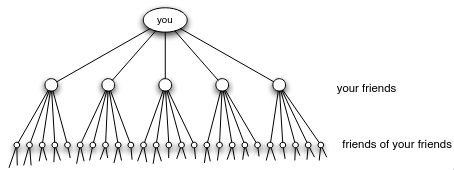
\includegraphics[width=\linewidth]{images/SMexp.png}
        \caption{\footnotesize Crescita puramente esponenziale delle conoscenze.}
    \end{subfigure}
    \hfill
    \begin{subfigure}[b]{0.45\linewidth}
        \centering
        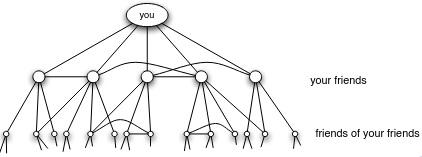
\includegraphics[width=\linewidth]{images/SMtriadic.png}
        \caption{\footnotesize La chiusura triadica diminuisce di molto il numero di persone raggiungibili con percorsi brevi.}
    \end{subfigure}
    \label{fig:sm_comparison}
\end{figure}

\subsection{Modello Watts - Strogatz}

Nel 1998 Duncan Watts and Steve Strogatz proposero un modello generativo di grafi aleatori che soddisfano due proprietà precedentemente viste: la presenza di numerosi triangoli e la presenza di cammini brevi che collegano le entità della rete.

Il grafo generato in accordo col modello Watts-Strogatz è composto da due componenti:
\begin{enumerate}
    \item una componente deterministica che consiste in una griglia bidimensionale
    \item una componente aleatoria sovrastante
\end{enumerate}

Il grafo fissato deterministicamente è una griglia "arricchita" - che corrisponde, sostanzialmente a uno Unit Disk Graph. I nodi sono considerati come punti in uno spazio metrico bidimensionale (un sottoinsieme di $\mathbb{N}^2$). Sono disposti sui punti a coordinate intere di un quadrato centrato nell'origine degli assi cartesiani e ogni nodo è collegato a ciascuno dei nodi vicini in orizzontale, verticale e diagonale.

\begin{definizione}[Griglia Arricchita]
    Fissato $n \in \mathbb{N}$. Un grafo a griglia "arricchita", è un grafo dove,    
    \begin{itemize}
        \item $V = \{(i, j) \in \mathbb{N}^2 : 0 \le i,j \le n \}$
        \item $E = \left\{ ((i,j),(a,b)) \in V^2 : [(a, b) = (i + \alpha,j + \beta): \alpha,\beta \in \{-1,0,1\}, (\alpha,\beta)\neq (0,0)]\right\}$
    \end{itemize}
\end{definizione}

Se si fa attenzione alla definizione di $E$ (ovvero l'insieme degli archi della componente deterministica), si può vedere che la griglia ha una sorta di \textit{periodicità}, ovvero i nodi a un bordo della griglia sono collegati ai nodi sul bordo opposto.
In questa maniera otteniamo un primo grafo con un'alta quantità di \textit{triangoli} (prima proprietà desiderata).

Per costruire la componente aleatoria fissiamo un $k>1$, e per ogni nodo $v \in V$ esso aggiungerà come ulteriori vicini altri $k$ nodi scelti \textbf{uniformemente a caso}.

\newpage

\begin{figure}[ht!]
    \centering
    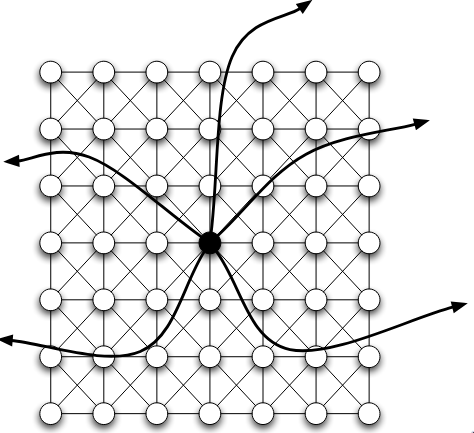
\includegraphics[width=0.5\linewidth]{images/SMWS.png}
    \caption{Watts-Strogatz}
\end{figure}

Come possiamo osservare, più che a una griglia su una superficie piana, dobbiamo pensare a \textbf{una griglia "appoggiata" su una superficie sferica}, che si racchiude su se stessa e che chiameremo \textbf{wrapped}.

Si può osservare una certa \textbf{dicotomia} tra gli archi deterministici e quelli aleatori:
\begin{enumerate}
    \item gli archi deterministici rappresentano un legame forte tra i nodi (\textbf{strong tie}), infatti tra due nodi legati da un arco deterministico esistono sempre dei triangoli. Possiamo dire che rappresentano delle relazioni "fisicamente" vicine.
    \item gli archi aleatori rappresentano invece delle conoscenze "alla lontana", e in quanto tale un legame debole (\textbf{weak tie}). Infatti è molto poco probabile trovare triangoli nella componente aleatoria (a meno che $k$ non sia molto grande).
\end{enumerate}

Ricapitolando, un grafo generato dal modello Watts-Strogatz contiene molti triangoli (\textbf{triadic closure}).
A questo punto rimane da chiederci se \textit{esistono numerosi cammini brevi tra i nodi della rete}.
Intuitivamente parlando, se si considerano cammini composti dai soli archi aleatori, è poco probabile incontrare due volte uno stesso nodo in brevi distanze. Successivamente \textit{Bollobàs e Ching} diedero una dimostrazione formale a questo fenomeno.
Più precisamente dimostrarono la presenza di cammini brevi in un modello con molta meno \textit{randomness}, individuando anche la lunghezza media degli shortest path nei grafi generati in accordo al modello di Watts-Strogatz. 

Consideriamo un nuovo modello simile a quello Watts-Strogatz, dove però solo un nodo su $k$ ha archi random, e il numero di archi random è pari a 1.
Partizioniamo poi la rete in "città" di $k \times k$ individui, e consideriamo il fenomeno small-world a livello di città.
Certamente ogni città avrà mediamente $k$ archi random, e inoltre ogni coppia di nodi $u,v$ di una stessa città sarà connessa da un cammino breve di lunghezza al più $2k$.

Venne dimostrato che per trovare un cammino relativamente corto tra due nodi $u,v$ di due città differenti, basta che $u$ raggiunga un nodo $w$ nella stessa città (in al più $2k$) passi, e poi tramite pochi salti passare da una città all'altra fino ad arrivare alla città di $v$.

In conclusione, anche con un piccolo ammontare di casualità, il modello Watts-Strogatz cattura il fenomeno "small-world".

\subsection{Navigabilità del modello Watts-Strogatz}

Supponiamo ora di essere il nodo $u$ in un grafo di Watts-Strogatz e vogliamo inviare un messaggio ad una certa destinazione $v$ \textbf{di cui conosciamo le coordinate}. Ovviamente, cerchiamo di fare arrivare il messaggio il più velocemente possibile, ossia cerchiamo di fare in modo che venga consegnato attraverso uno shortest path da $u$ a $v$. Poiché noi (nodo $u$) non conosciamo altro della rete se non i nostri vicini, facciamo tante copie del messaggio quanti sono i vicini e mandiamo una copia a ciascun vicino (al più 8/9 messaggi, numero costante). Ovviamente, potremmo procedere in modo diverso, ovvero potremmo scegliere, fra i nostri vicini quello le cui coordinate sono più prossime a quelle di $v$, ma la casualità dei weak ties potrebbe far si che, invece, un vicino che, al momento, mi appare peggiore ha un arco random che lo collega direttamente a $v$.

\begin{figure}[ht!]
    \centering
    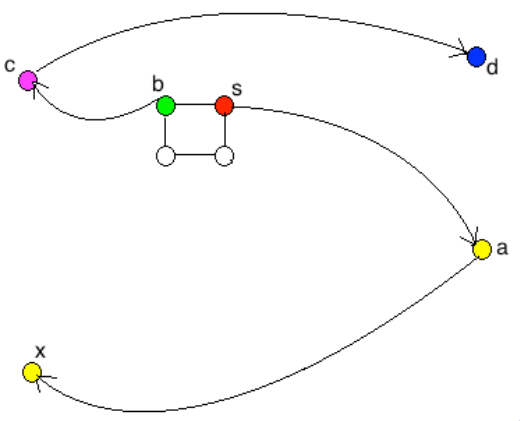
\includegraphics[width=0.5\linewidth]{images/SMexample.png}
    \caption{Esempio di navigabilità del grafo di WS}
    \label{fig:ex_navigabilità}
\end{figure}

Osservando la \autoref{fig:ex_navigabilità}, il nodo $s$ deve inviare un messaggio a $d$. Fra i vicini di $s$ il più vicino a $d$ \textbf{sulla griglia} è $a$, perché $b$ \textbf{sulla griglia} è più lontano di $a$ da $d$, e queste sono le uniche informazioni di cui $s$ è in possesso. Perciò, $s$ inoltra il messaggio ad $a$, che poi dovrà seguire i nodi della griglia per giungere a $d$. Supponiamo invece che $s$ avesse inoltrato il messaggio a $b$, in questo modo si sarebbe allontanato \textbf{sulla griglia} da $d$, ma avrebbe raggiunto $d$ in soli 3 passi, infatti il messaggio avrebbe seguito il percorso $s \rightarrow c \rightarrow a$ invece che $s \rightarrow a \rightarrow \dots \rightarrow d$.

Il nodo $u$ deve inviare un messaggio al nodo $v$. Per farlo, $u$ crea tante copie del messaggio quanti sono i suoi vicini, e ne invia una a ciascuno di essi.
Ciascun vicino, a sua volta, replica lo stesso comportamento: genera tante copie del messaggio quanti sono i propri vicini e le inoltra a tutti loro.
Il processo continua in questo modo iterativamente.
Dopo $h$ passi, nel grafo circolano $\approx 7^h$ copie del messaggio.
Questa procedura è nota come \textbf{flooding}. È evvidente che il numero di messaggio è inaccettabile, inoltre nel esperimento di Milgram, ad ogni passo circolavano tanti messaggi quanti ne aveva creati Milgram, e non aumentavano ad ogni passo (no \textbf{flooding}, eppure gli individui che parteciparono all'esperimento di Milgram avevano la stessa conoscenza dei nodi del modello di WS). Notiamo quindi, che il modello di WS non riesce a descrivere qualche caratteristica di una rete sociale che rende possibile la ricerca di Milgram.

\subsubsection{Ricerca decentralizzata (ricerca miope)}

Vogliamo un modo per trovare un cammino non troppo lungo tra $u$ e $v$ in modo da trasmettere una sola copia del messaggio, e non un numero esponenziale, un po' come fecero le persone che parteciparono all'esperimento di Milgram.

Purtroppo fare questo tipo di ricerca \textbf{miope} in un modello Watts -Strogatz non è possibile, e lo abbiamo visto negli esempi discussi sopra. Nell'esperimento di Milgram, gli individui coinvolti hanno utilizzato un algoritmo di ricerca decentralizzata, che in quel caso si dimostrava efficiente. Probabilmente, ad ogni passo, un individuo inoltrava la copia della lettera in suo possesso a quello fra i suoi contatti che stimava essere più vicino possibile al destinatario, dove "più vicino" può riferirsi a metriche diverse: più vicino geograficamente, o rispetto alla professione, a agli interessi culturali etc... .

Inoltre è stato anche dimostrato con questo tipo di ricerca (nota come \textbf{ricerca decentralizzata}), non solo non c'è nessuna garanzia di trovare un cammino corto, ma mediamente i cammini trovati sono molto più lunghi dei cammini minimi che esistono tra mittente e destinatario.

Sostanzialmente il problema è che gli archi random della componente aleatoria sono "troppo" casuali per dare un supporto alla ricerca decentralizzata.
Infatti in un contesto sociale reale, è molto poco probabile che due persone totalmente a caso entrino in contatto.

È invece più probabile avere archi casuali tra persone più vicine fisicamente, anziché tra persone molto lontane.

Quindi possiamo dire che questo modello non è navigabile, e quindi non rispecchia le caratteristiche volute.

\subsection{Un modello per la ricerca decentralizzata}

Vogliamo ora definire un modello generativo cui corrispondano grafi che contengono molti triangoli e nei quali esistono shortest paths fra le coppie di e nei quali \textbf{trovare gli shortest path mediante ricerca decentralizzata sia possibile}. Il nuovo modello è ancora basato sul grafo a griglia arricchita del modello WS, ma ora la probabilità che l'arco random uscente dal nodo $u$ sia $(u, v)$ è inversamente proporzionale alla distanza \textbf{sulla griglia} dei nodi $u$ e $v$, quindi
\[
\Pr[(u, v) \in E] = \frac{1}{Z_u} \frac{1}{d(u, v)^q}
\]
dove $d(u, v)$ indica la lunghezza di uno shortest path fra $u$ e $v$ \textbf{sulla griglia} (percorso che non contiene archi random), mentre $Z_u$ è un fattore di normalizzazione.

Poiché da ogni nodo deve uscire uno e un solo arco random, deve valere che:
Fissato un nodo $u \in V$, si assume che esso scelga un nodo $v \in V - \{u\}$ a cui connettersi in modo equiprobabile. Di conseguenza, la probabilità che esista un arco $(u,v)$ è la stessa per tutti i nodi $v \neq u$, e la somma di tali probabilità è pari a 1.

\begin{align*}
&\sum_{v \in V - \{u\}} \Pr[(u, v) \in E] 
    = \sum_{v \in V - \{u\}} \frac{1}{Z_u} \frac{1}{d(u, v)^q} = 1 \\
&\implies\quad 
Z_u = \sum_{v \in V - \{u\}} \frac{1}{d(u, v)^q}
\end{align*}

In pratica, poiché la griglia è simmetrica, allora $Z_u$ ha lo stesso valore per tutti i nodi e, pertanto, indicheremo il fattore di normalizzazione, semplicemente, come $Z$.

Il parametro $q$ invece prende il nome di \textbf{esponente di clustering}. Con $q = 0$, otteniamo il modello di WS. In generale, gli archi random sono "troppo random" quando $q$ è piccolo, "non abbastanza random" quando $q$ è grande. Ovviamente, la ricerca decentralizzata funziona meglo con alcune scelte di $q$ e peggio con altre. Quello che vogliamo ora mostrare è che esiste una scelta di $q$ che rende efficiente la ricerca decentralizzata, ossia, permette di trovare percorsi la cui lunghezza non è troppo lontana da quella
degli shortest paths.

È possibile però dimostrare, che data una griglia $d$-dimensionale wrapped, allora il componente di clustering ottimale sarà esattamente $q = d$.

Cerchiamo ora di dare una spiegazione intuitiva a questo fenomeno.
Riconsideriamo nuovamente l'esperimento di Milgram, dove però abbiamo il mittente $A$ che vive negli Stati Uniti mentre il destinatario $B$ vive a Roma quartiere Garbatella.
Certamente la prima cosa che farebbe $A$ sarebbe quella di inviare la lettera quantomeno ad una persona che vive in Europa.
Anche se $A$ non ha amici diretti in Europa a cui inviare la lettera, passandola ad altri amici negli USA troverà brevemente qualcuno che ha amici che vivono oltre oceano.
Per semplicità assumiamo che $A$ invii direttamente la lettera ad un suo amico $C$ che vive a Mosca.
A sua volta $C$ cerca tra i suoi amici qualcuno che abiti almeno in Europa Occidentale.
Da $C$ la lettera passa a $D$ che vive a Parigi.
Per fortuna $D$ ha un amico in Italia che però vive a Perugia, e quindi la lettera finisce in Umbria. $D$ si ricorda di avere un lontano parente $E$ nel Lazio, a cui invia la lettera.
Dopodiché $E$ invia la lettera ad un suo collega $F$ che abita a Roma Centocelle, il quale a sua volta invierà la lettera a un amico $G$ che abita a Garbatella.
Di li, sicuramente in un numero non esagerato di passi la lettera arriva a $B$.
Come si può intuire, il processo di ricerca decentralizzata procede per \textbf{scale di risoluzione}. Infatti, anche se per pochi salti la lettera percorre relativamente poca distanza, presto farà un salto che riduce drasticamente la distanza con la destinazione.

\begin{teorema}[Informale: Coefficiente di clustering ottimale per $d = 2$]
    Se la componente deterministica del grafo è una griglia bidimensionale $(d = 2)$, allora l'esponente di clustering ottimale è $q = 2$.
\end{teorema}
\begin{proof}
    Fissiamo un nodo $u$, e partizioniamo gli altri nodi in “anelli” concentrici intorno a $u$, in modo che la distanza cresca esponenzialmente.  
    In particolare, consideriamo i nodi con distanza da $u$ nell'intervallo:
    \[
    [2^h, 2^{h+1}), \quad h = 0, 1, 2, \dots
    \]
    
    Dato che i punti su una circonferenza crescono come il quadrato del raggio, il numero di nodi nell'intervallo $[2^h, 2^{h+1})$ sarà proporzionale a $2^{2h}$. Definiamo:
    \[
    A_h = \{x : 2^h \leq d(u,x) < 2^{h+1}\} \implies |A_h| = \pi (2^{h+1})^2 - \pi (2^h)^2 = 3 \pi 2^{2h}.
    \]
    
    Ora, la probabilità che un nodo $v$ a distanza $r \approx 2^h$ venga scelto come destinazione di un arco casuale da $u$ è:
    \[
    \Pr[v \text{ scelto}] \approx \frac{1}{d(u,v)^q} \approx 2^{-hq}.
    \]
    
    Di conseguenza, la probabilità che l'arco casuale cada in un blocco $A_h$ è:
    \[
    \Pr[A_h] \approx |A_h| \cdot 2^{-hq} \approx 2^{2h} \cdot 2^{-hq} = 2^{(2-q)h}.
    \]
    
    Vediamo cosa succede per diversi valori di $q$:
    \renewcommand{\arraystretch}{1.5}
    \begin{table}[h!]
    \centering
    \begin{tabular}{|c|c|c|}
    \hline
    \textbf{Valore di $q$} & $P(A_h) \approx 2^{(2-q)h}$ & \textbf{Significato} \\
    \hline
    $q < 2$ & $P(A_h)$ \textbf{aumenta} con $h$ & troppi archi lunghi \\
    \hline
    $q > 2$ & $P(A_h)$ \textbf{diminuisce} con $h$ & troppi archi corti \\
    \hline
    $q = 2$ & $P(A_h) \approx 2^{(2-2)h} = 2^0 = 1$ & \textbf{indipendente da $h$} \\
    \hline
    \end{tabular}
    \caption{Comportamento della probabilità $P(A_h)$ in funzione del parametro $q$}
    \end{table}
    
    Da questa analisi si vede che il valore ottimale è $q = 2$, poiché la probabilità $\Pr[A_h]$ risulta uniforme su tutti gli anelli, evitando sia archi troppo lunghi che troppo corti.
\end{proof}

Quindi, \textbf{i weak ties sono distribuiti uniformemente su tutte le scale di risoluzione}, e questo fa sì che, anche se per un certo numero di passi occorre utilizzare gli archi della griglia (perché gli archi random che si incontrano fanno allontanare dall'obiettivo, e, dunque, ad ognuno di questi passi ci si avvicina solo di un'inezia all'obiettivo) non occorreranno molti passi prima di arrivare ad un nodo il cui arco random diminuisce \textbf{drasticamente} la distanza dall'obiettivo (di un ordine di grandezza!).

\subsubsection{Prestazioni della ricerca miope (decentralizzata)}

Nella precedente sezione abbiamo dato un'idea intuitiva del perché una distribuzione inversamente quadratica dei weak ties rispetto alle distanze rende la ricerca decentralizzata possibile.

Per semplicità verrà fatta un'analisi rigorosa (e non intuitiva) di questo fenomeno su una griglia 1-dimensionale, ovvero un anello.

\begin{figure}[ht!]
    \centering
    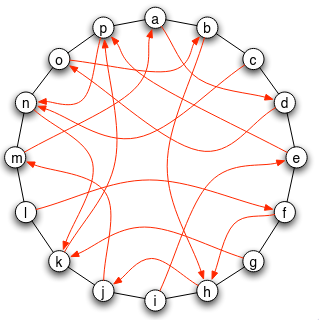
\includegraphics[width=0.3\linewidth]{images/SManello.png}
    \caption{Anello con random links}
\end{figure}

Consideriamo un grafo $G$ tale che:
\begin{itemize}
    \item $V = [n]$
    \item $E_d = \{(i, i+1) \in V: 1 \leq i < n\ \cup\ \{n, 1\}\}$, rappresentando la componente deterministica di partenza.
\end{itemize}
Quindi, in finale
\[
E = E_d \cup \left\{(u,v) \in V: \Pr[(u, v) \in E] = \frac{1}{Z} \frac{1}{d(u, v)}\right\}
\]
Sapendo quindi che $q = 1$, allora per ogni $u \in V$
\[
Z = \sum_{v \in V - \{u\}}\frac{1}{d(u, v)} \underbrace{=}_{(1)} 2 \sum_{1 \leq h \leq \frac{n}{2}} \frac{1}{h} \leq 2 \sum_{h = 1}^{\infty}\frac{1}{h} = 2 \ln n 
\]
\[
\implies Z \leq 2 \ln n
\]

Vale la \textbf{(1)} perché in un anello, il nodo $u$ ha due vicini a distanza 1, due vicini a distanza 3, e cosi via... .

\begin{osservazione}[Fasi dell'algoritmo]\label{oss:fasi}
    
Scegliamo uniformemente a casa due nodi $s$ e $t$ in $G$ ed utilizziamo l'algoritmo di ricerca decentralizzata per calcolare un percorso da $s$ a $t$. Indichiamo con $X$ la variabile aleatoria che denota la lunghezza di tale percorso e sia $\mathbb{E}[X]$ la lunghezza media di tali cammini.
Considerando una ricerca miope da $s$ a $t$, diremo che essa si trova della fase $j$ se il messaggio si trova ad una distanza compresa tra $2^j$ e $2^{j+1}$ dal destinatario. Poiché la distanza tra due nodi nell'anello è al più $\frac{n}{2}$, allora il numero massimo di fasi è al più $\log_2n$. Possiamo scrivere $X$ come la somma delle v.a. $X_1, X_2, \dots, X_{\log_2}$ dove $X_i$ è la lunghezza complessiva del cammino lungo la fase $i$
\[
X = X_1 + X_2 + \dots + X_{\log_2}
\]

Per linearità avremo che
\[
\mathbb{E}\left[ X \right] = \mathbb{E}\left[ X_1 + X_2 + ... + X_{\log_2{n}} \right] = \mathbb{E}\left[ X_1 \right] +  \mathbb{E}\left[ X_2 \right] + ... +  \mathbb{E}\left[ X_{\log_2{n}} \right]
\]
\end{osservazione}

\begin{teorema}
    Sia $\mathbb{E}\left[ X \right]$ la lunghezza media dei cammini risultati dalla ricerca miope tra una qualsiasi coppia di nodi, allora 
    \[
    \mathbb{E}\left[ X \right] \in O(\log^2{n})
    \]
\end{teorema}
\begin{proof}
    Siano i nodi $s,\ t$ rispettivamente il nodo \textbf{mittente} e il nodo \textbf{destinatario}. Abbiamo partizionato i nodi in base a distanze dalla sorgente $t$ che si \textit{dimezzano}, ovvero abbiamo definito la fase $j$ in cui il messaggio appartiene a un nodo $u$ con distanza
\[
\frac{d(s,t)}{2^{j+1}} \leq d(u,t) < \frac{d(s,t)}{2^j}
\]

Ricordando che il numero di fasi è al più $\log_2n$, e per quanto visto nella \autoref{oss:fasi}, per dimostrare il teorema è, quindi sufficiente dimostrare che:
\[
\forall j,\ \mathbb{E}[X_j] \in O(\ln n).
\]

Supponiamo di trovarci nel nodo $v$ durante la fase $j$, allora
\[
\frac{d(s,t)}{2^{j+1}} \leq d(v,t) < \frac{d(s,t)}{2^j}
\]
La fase $j$, termina sicuramente se esiste un nodo $z$ tale che
\[
(v, z) \in E\ \land d(z, t) \leq \frac{d(v, t)}{2} \leq \frac{1}{2} \frac{d(s, t)}{2^j} = \frac{d(s, t)}{2^{j + 1}} 
\]
Ovvero, sicuramente esiste quel arco $(v, z)$ che ci permette di dimezzare la distanza, e quindi passare nella prossima fase. Quindi
\begin{align*}
\Pr[\text{fase $j$ termina}] &= \Pr\left[\exists z \in V: (v, z) \in E \land d(z, t) \leq \frac{d(s, t)}{2^{j + 1}}\right] \\
&\underbrace{\geq}_{(1)} \Pr\left[\exists z \in V: (v, z) \in E \land d(z, t) \leq \frac{d(z, t)}{2} \right] 
\end{align*}
Vale la \textbf{(1)}, in quanto potrebbe essere che $d(v, t) = \frac{d(s, t)}{2^j}$, in tal caso, esisterebbe un arco $(v, z)$ nell'anello, tale che $d(z, t) = d(v, t) - 1 < \frac{d(s, t)}{2^j}$, e tale arco farebbe certamente terminare la fase $j$, e tuttavia sarebbe $d(z, t) > \frac{d(v, t)}{2}$ \textbf{(DA CAPIRE)}.

Indichiamo con $I$, l'insieme dei nodi che distano da $t$ non più della metà di quanto $v$ dista da $t$, ovvero:
\[
I = \left\{ u \in V: d(u, t) \leq \frac{d(v,t)}{2} \right\}
\]
Allora, 
\setlength{\jot}{10pt} % aumenta lo spazio verticale tra le righe
\begin{align*}
&\Pr\left[\exists z \in V: (v, z) \in E \land d(z, t) \leq \frac{d(z, t)}{2} \right] = \Pr\left[\exists z \in I: (v, z) \in E\right]\\
&= \Pr[\exists z \in I: (v, z) \text{ è un arco dell'anello oppure è un arco random}] \\
&= \sum_{z \in I}\Pr[(v, z) \text{ è un arco dell'anello oppure è un arco random}] \\
&\geq \sum_{z \in I}\Pr[(v, z) \text{ è un arco random}] = \sum_{z \in I}\frac{1}{Z}\frac{1}{d(v, z)}
\end{align*}
Dobbiamo ora stimare quanto vale $d(v, z)$. Certamente $v$ può raggiungere $z$ tramite un cammino del tipo $v \rightarrow t \rightarrow z$, e questo cammino sarà almeno lungo $d(v, z)$.
\[
d(v, z) \leq d(v, t) + d(t, z) = d(v, t) + d(z, t) \leq d(v, t) + \frac{d(v, t)}{2} = \frac{3d(v, t)}{2}
\]
Allora, per ogni $z \in I$,
\begin{align*}
    \sum_{z \in I}\Pr[(v, z) \text{ è un arco random}] &= \sum_{z \in I}\frac{1}{Z}\frac{1}{d(v, z)} \\ &\geq \sum_{z \in I} \frac{1}{Z}\frac{2}{3d(v, t)} \\ &\geq \sum_{z \in I}\frac{1}{2\ln n} \frac{2}{3d(v, t)} \\ &= \sum_{z \in I}\frac{1}{3d(v, t) \ln n} \\
    &= \frac{1}{3d(v, t)\ln n} |I|
\end{align*}

Dunque,
\[
\Pr\left[\exists z \in V: (v, z) \in E \land d(z, t) \leq \frac{d(z, t)}{2} \right] \geq \frac{1}{3d(v, t)\ln n} |I|
\]


Resta da valutare quanto vale $|I| = \left|\left\{ u \in V: d(u, t) \leq \frac{d(v, t)}{2} \right\}\right|$. 
Siano $v_{sin}$ e $v_{des}$ i due nodi in $I$ a distanza massima da $t$. Allora,

\[
d(v_{sin}, t) = d(v_{des}, t) = \left\lfloor\frac{d(v, t)}{2}\right\rfloor
\]

\begin{figure}[ht!] \centering 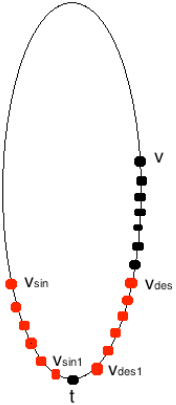
\includegraphics[width=0.2\linewidth]{images/Vsin_Vdes.png} \end{figure}


Ci prendiamo la parte intera inferiore, perché $\frac{d(v, t)}{2}$ potrebbe non essere intero. 
Siano ora $v_{sin_1}$ e $v_{des_1}$ i due nodi adiacenti a $t$. 
Allora $I$ contiene:
\begin{enumerate}
    \item Il nodo $t$
    \item gli $\left\lfloor\frac{d(v, t)}{2}\right\rfloor$ nodi da $v_{sin}$ a $v_{sin_1}$
    \item gli $\left\lfloor\frac{d(v, t)}{2}\right\rfloor$ nodi da $v_{des}$ a $v_{des_1}$
\end{enumerate}
Quindi,
\[
|I| = 1 + \left\lfloor\frac{d(v, t)}{2}\right\rfloor + \left\lfloor\frac{d(v, t)}{2}\right\rfloor 
\geq 1 + \frac{d(v, t) - 1}{2} + \frac{d(v, t) - 1}{2} = d(v, t)
\]

Riassumendo, l'obiettivo è di dimostrare che $\forall\ j,\ \mathbb{E}[X_j] \in O(\ln n)$.
Abbiamo ottenuto che 
\[
\Pr[\text{fase $j$ termina}] \geq \frac{1}{3d(v, t)\ln n} d(v, t) = \frac{1}{3 \ln n} 
\]
Quindi, 
\[
\Pr[\text{fase $j$ non termina}] \leq 1 - \frac{1}{3 \ln n}
\]
Quindi, la probabilità che non termini in $h$ passi è:
\[
\Pr[X_j \geq h] = \Pr[\text{fase $j$ \textbf{non} termina per $h$ passi}] \leq \left[1 - \frac{1}{3 \ln n}\right]^h 
\]

Per concludere, non resta che calcolare che $\mathbb{E}[X_j]$.
\begin{align*}
\mathbb{E}[X_j] &= 1 \cdot \Pr[X_j = 1] + 2 \cdot \Pr[X_j = 2] + \dots + \frac{n}{2} \cdot \Pr[X_j = \underbrace{\frac{n}{2}}_{d(s, t) \leq \frac{n}{2}}] \\
&= \Pr[X_j \geq 1] + 1 \cdot \Pr[X_j = 2] + \dots + (\frac{n}{2} - 1) \cdot \Pr[X_j = \frac{n}{2}] \\
&= \Pr[X_j \geq 1] + \Pr[X_j \geq 2] + 1 \cdot \Pr[X_j = 3] \dots + (\frac{n}{2} - 2) \cdot \Pr[X_j = \frac{n}{2}] \\
&=\dots \\
&= \sum_{1 \leq h \leq \frac{n}{2}} \Pr[X_j \geq h]
\end{align*}

A questo punto, abbiamo che
\begin{align*}
\mathbb{E}[X_j] &= \sum_{1 \leq h \leq \frac{n}{2}} \Pr[X_j \geq h] \leq \sum_{1 \leq h \leq \frac{n}{2}} \left[1 - \frac{1}{3 \ln n}\right]^h \\
& \leq \sum_{h \geq 0} \left[1 - \frac{1}{3 \ln n}\right]^h \underbrace{=}_{(1)} \frac{1}{1 - \left[1 - \frac{1}{3 \ln n}\right]} = 3 \ln n \\
\end{align*}
Vale la \textbf{(1)}, perché è stata riconosciuta una serie geometrica di ragione $q = \left[1 - \frac{1}{3 \ln n}\right]$, ricordando che la serie geometrica vale:
\[
\sum_{n = 0}^{\infty} q^n = \frac{1}{1 - q}
\]
Per concludere la dimostrazione, abbiamo che
\[
\mathbb{E}[X] = \sum_{1 \leq j \leq \log_2n} E[X_j] \leq \sum_{1 \leq j \leq \log_2n} 3 \ln n = \log_2 n \cdot 3 \ln n = \log_2 e \cdot \ln n \cdot 3 \ln n \in O(\ln^2 n) 
\]
\end{proof}

\newpage
\subsubsection{Perché $q = d$ funziona bene in $\mathbb{R}^d$}

Nel modello di Kleinberg, i nodi sono disposti su una griglia $d$-dimensionale, e ogni nodo $v$ è connesso:
\begin{itemize}
    \item ai \textit{vicini locali}, cioè ai nodi adiacenti nella griglia;
    \item a uno o più \textit{collegamenti di lungo raggio}, scelti con probabilità proporzionale a $\frac{1}{d(v,u)^q}$.
\end{itemize}

Il parametro $q$ controlla quanto le connessioni siano locali o globali: per $q$ piccolo, prevalgono archi lunghi; per $q$ grande, la rete è quasi regolare. L'obiettivo è capire per quale valore di $q$ la \textit{ricerca decentralizzata} (greedy routing) risulta efficiente, cioè richiede un numero di passi polilogaritmico per raggiungere una destinazione $t$.

In un anello, il numero di nodi entro distanza $d(v,t)$ è $|I| \approx d(v,t)$, mentre il fattore di normalizzazione è
\[
Z = \sum_{u \neq v} \frac{1}{d(v,u)} \le 2 \ln n.
\]
La probabilità che $v$ abbia un vicino $z$ tale che $d(z,t) \le \frac{d(v,t)}{2}$ è
\[
\Pr[\exists z: (v,z)\in E,\, d(z,t)\le\tfrac{d(v,t)}{2}] \ge \frac{1}{3\ln n},
\]
che è indipendente da $d(v,t)$. La ricerca può quindi procedere con una probabilità costante di avvicinarsi a $t$, risultando in un tempo atteso $O(\log^2 n)$.

In una griglia 2D, il numero di nodi entro distanza $d(v,t)$ cresce come l'area di un quadrato di lato $\approx d(v, t)$:
\[
|I| = \alpha\, d(v,t)^2,
\]
e il fattore di normalizzazione è
\[
Z = \sum_{u \neq v} \frac{1}{d(v,u)^2} \le \beta \ln n.
\]
Si ottiene così
\[
\Pr[\exists z: (v,z)\in E,\, d(z,t)\le\tfrac{d(v,t)}{2}] 
\ge \frac{4\alpha}{9\beta\ln n},
\]
ancora una volta indipendente da $d(v,t)$, e quindi la ricerca rimane efficiente.

In generale, in $\mathbb{R}^d$ la ricerca decentralizzata è efficiente se e solo se $q = d$.  
Solo in questo caso, il numero di nodi a distanza $\le d(v,t)$ cresce come $d(v,t)^d$ e il fattore di normalizzazione $Z$ cresce come $\ln n$, bilanciando perfettamente collegamenti locali e globali.  

Se $q < d$, le connessioni lunghe sono troppo frequenti e la rete perde struttura;  
se $q > d$, le connessioni sono troppo locali e la ricerca diventa lenta.  
Per $q = d$, invece, la rete è \textbf{navigabile}: mantiene la proprietà di small-world e consente una ricerca efficiente e decentralizzata.

\newpage
\subsubsection{Perché $q \neq d$ funziona male in $\mathbb{R}^d$}

Consideriamo il caso unidimensionale ($d = 1$) con $q = 0$. In questo scenario, la probabilità di scegliere un arco random $(u,v)$ è uniforme:
\[
\mathcal{P}((u,v) \in E) = \frac{1}{Z}\frac{1}{d(u,v)^0} = \frac{1}{Z}, \quad \text{dove} \quad Z = \sum_{v \neq u}\frac{1}{d(u,v)^0} = n - 1.
\]
Quindi, ogni arco random compare con probabilità $\frac{1}{n-1} > \frac{1}{n}$.

Definiamo ora l'insieme dei nodi entro distanza al più $\sqrt{n}$ dal destinatario $t$:
\[
R = \{ x \in V : d(x,t) \leq \sqrt{n} \}.
\]
Per un nodo $u \notin R$, la probabilità di connettersi tramite un arco random a un nodo di $R$ è:
\[
\Pr[\exists (u,v) \in E : v \in R] = \sum_{v \in R} \frac{1}{n} = \frac{|R|}{n} = \frac{2}{\sqrt{n}}.
\]

Sia $Y$ la variabile aleatoria che indica il numero di passi necessari per raggiungere $R$ partendo da $u$. Si ha:
\[
\Pr[Y \geq h] < \left(1 - \frac{2}{\sqrt{n}}\right)^h,
\quad
\mathbb{E}[Y] \leq \frac{1}{1 - \left(1 - \frac{2}{\sqrt{n}}\right)} = \frac{\sqrt{n}}{2}.
\]
Questo valore è già esponenzialmente più grande rispetto al tempo di ricerca miope nel caso $q=1$.

Per $q > 1$, gli archi random diventano più corti e la ricerca non migliora; per $q$ molto grande, la rete tende a ridursi alla sola componente deterministica.

\begin{teorema}
Sia $X$ la variabile aleatoria che rappresenta la lunghezza del cammino trovato dalla ricerca miope su un anello di $n$ nodi.  
Per ogni $q \neq 1$ esistono costanti $\alpha_q, c_q > 0$ tali che:
\[
\mathbb{E}[X] \geq \alpha_q \cdot n^{c_q}.
\]
\end{teorema}

Questi risultati, dimostrati per $d=1$, si estendono a dimensioni maggiori $d > 1$ con argomentazioni analoghe ma più complesse.

\chapter{Teoria dei grafi e delle reti sociali}

\section{Esperimento di Granovatter}

Nel 1960, il sociologo Mark Granovetter effettuò il seguente esperimento nella sua tesi di dottorato: intervistò una serie di persone che di recente avevano cambiato lavoro, facendo domande poste a capire in che modo erano venuti a conoscenza della nuova opportunità lavorativa.

Come ci si può aspettare la gran parte delle persone erano venuti a conoscenza dell'opportunità da lavoro tramite passaparola.

Ciò che invece era meno atteso, è che un gran numero di volte l'informazione arrivò da gente che si conosceva superficialmente.
Questo fu sorprendente perché ci si aspetta che gli amici più stretti siano quelli più interessati ad aiutarsi nel momento del bisogno.

Una risposta al fenomeno proposta da Granovetter fu che le persone a noi strette in realtà tendono ad avere le stesse nostre informazioni.
Infatti è normale che se frequentino più o meno gli stessi posti e persone di un amico stretto.
Oppure, se ho una relazione stretta con una persona è perché ci ho parlato molto nel tempo, e quindi tutte le informazioni importanti che tale persona poteva darmi me le avrà già date in passato.

Contrariamente, una persona che conosco poco probabilmente frequenterà altri posti e persone, e quindi avrà accesso ad altre fonti di informazioni che provengono al di fuori della mia comunità.

\subsection{Bridge \& Local Bridges}

Consideriamo il grafo $G = (V, E)$ che modella la rete, gli archi che "aumentano" le nostre informazioni sono quelli che ci collegano a regioni della rete \textit{inaccessibili} ai nostri amici.

\begin{definizione}[Bridge]
    Definiamo un \textbf{bridge} come un arco la cui rimozione rende la rete disconnessa. Dall'esperimento di Granovatter, segue che i bridge sono gli archi che hanno maggione "valore informativo".
\end{definizione}

In una rete sociale reale (e artificiale) è davvero molto poco probabile che esistano bridge edges, anche perché sappiamo già che le reti sociali presentano delle componenti giganti con buona probabilità. Dobbiamo quindi rilassare le definizione di bridge.

\begin{definizione}[Local Bridge]
    Definiamo \textbf{local bridge} un arco $(u,v)$ se $u$ e $v$ non hanno altri amici in comuni, ovvero se $N(u) \cup N(v) \equiv \emptyset$
    
    Possiamo vedere i local bridge come archi la cui rimozione aumenta la distanza tra le due estremità di almeno 2.
\end{definizione}

\subsection{Weak \& Strong Ties}

Dall'esperimento di Granovatter, oltre a identificare il potere "informativo" degli archi, mostra anche che l'informazione arriva da qualcuno conosciuto solo superficialmente, e non dagli amici stretti. Possiamo quindi identificare due tipologie di relazioni: 
\begin{itemize}
    \item \textbf{Relazione Forte (Strong Tie)}: sono quelle relazioni che ci collegano agli amici stretti.
    \item \textbf{Relazione Debole (Weak Tie)}: sono quelle relazioni che ci collegano ai semplici conoscenti.
\end{itemize}
Di conseguenza, possiamo modellare una rete di questo tipo mediano un grafo $G$, in cui gli archi sono partizionati in due sottoinsiemi:
\[
G = (V, S \cup W) \text{ con } S \cap W = \emptyset
\]
E come ha mostrato l'esperimento di Granovatter, gli archi deboli veicolano informazioni alle quali non avremmo accesso tramite gli archi forti, e questa è la \textbf{forza degli archi deboli}.

\subsection{Strong Triadic Closure Property}

Consideriamo lo stato di una rete sociale in un dato istante, sarebbe interessante sapere come si evolve nel tempo e quali sono i meccanismi che portano alla creazione o alla rottura di nuovi archi.

Un principio abbastanza intuitivo è il seguente: se due nodi hanno un amico stretto in comune, allora è molto probabile che in futuro entrino in contatto e stabiliscano anch'essi un rapporto di amicizia stretta. Ciò che si genera quindi tra i tre nodi in questione è la cosiddetta \textbf{chiusura triadica}.

Pensando la chiusura triadica in termini di strong e weak ties possiamo definirla secondo la seguente regola:
\begin{definizione}[Chiusura Triadica]
Sia il nodo $a$ e due suoi vicini $b$ e $c$, allora l'arco $(b,c)$ probabilmente si creerà se $(a,b),\ (a,c) \in S$, ovvero se sono una \textbf{strong tie}.
\end{definizione}

\begin{definizione}[Strong Triadic Closure Property (STCP)]
Sia $G = (V, S\cup W)$; un nodo $u$ soddisfa la \textbf{proprietà della chiusura triadica forte} se, per ogni coppia di archi incidenti su $u$, i loro estremi sono collegati da un arco. Formalmente:
\[
u \in V \text{ soddisfa la STCP } \iff \forall(u, v),(u, w) \in S: [(v, w) \in S \cup W]
\]
$G$ soddisfa la STCP se tutti i nodi la soddisfano.
\end{definizione}
Se si osserva bene, quando una rete soddisfa la STCP essa si \textbf{stabilizza} secondo la regola precedentemente descritta, ovvero in futuro non si genereranno più altri archi.

\subsection{STCP \& Local Bridges}

\begin{teorema}
    Sia $G=(V, S \cup W)$; se un nodo $u \in V$ soddisfa la STCP e se esistono due nodi distinti $x$ e $z$ tali che $(u, x) \in S$ e $(u, z)$ è un local bridge (ovvero $N(u) \cap N(z) = \emptyset$), allora $(u,z) \in W$, ovvero è un weak tie (arco debole).
\end{teorema}
\begin{proof}
    Poiché $(u,z)$ è un local bridge, allora $N(u) \cap N(z) = \emptyset$ (per definizione di local bridge). Se per assurdo $(u, z) \in S$, allora, poiché $(u,x) \in S$ e $u$ soddisfa la STCP, dovrebbe esistere l'arco $(x, z) \in S \cup W$, ossia sarebbe che che $x \in N(u) \cap N(z)$ che per ipotesi è uguale all'insieme vuoto - \textbf{Assurdo!}
\end{proof}

Questo teorema mostra come \textit{una proprietà globale (essere un local bridge) si riflette in una proprietà locale (essre un weak tie)}. Infratti:
\begin{itemize}
    \item Essere weak tie è proprietà locale: un nodo sa da solo se un suo vicino è un amico o un conoscente.
    \item Essere local bridge è una proprietà globale: un nodo deve chiedere a tutti i suoi vicini se qualcuno di loro conosce un suo conoscente per sapere se è un local bridge.
\end{itemize}

Infatti, nell'esperimento di Granovetter, i weak ties, in quanto portatori di informazioni erano anche local bridges.

\subsection{Comunità e Coefficiente di Clustering}

Abbiamo definito in precedenza un modello di rete dinamica i cui archi si modificano nel tempo, e dove la rete si stabilizza nel momento in cui essa soddisfa la Proprietà Forte di Chiusura Triadica.

Dato che si generano tanti triangoli, allora nel grafo stabilizzato si creeranno gruppi di nodi \textbf{fortemente coesi} da una densa quantità di archi.
Chiameremo questi gruppi fortemente coesi \textbf{comunità}, o \textbf{cluster}.

La precedente è una definizione informale e discorsiva.
Dal punto di vista formale, quando possiamo dire che un gruppo di nodi è abbastanza coeso da essere definito comunità?
E che significa \textbf{coeso}?
Per fare ciò iniziamo col \textbf{quantificare} la coesione del nodo $u$ all'interno dei suoi vicini.

\begin{definizione}[Coeffiecente di Clustering]
    Definiamo il \textbf{coefficiente di clustering} $c(u)$ come il rapporto fra il numero di relazioni fra i vicini di $u$ rispetto a tutte le coppie possibili di vicini di $u$:
    \[
    c(u) = \frac{|\{(x,y) \in E: x \in N(u) \land y \in N(u)\}|}{\frac{|N(u)| \cdot (|N(u)| - 1)}{2}}
    \]
\end{definizione}

Informalmente, il coefficiente di clustering misura quanto un nodo è "ben inserito" all'interno della rete costituita dai suoi vicini.
\begin{itemize}
    \item Un nodo con coefficiente di clustering basso è "male" inserito nel gruppo dei suoi amici, in quel gruppo si trova in una posizione periferica.
    \item Un nodo con coefficiente di clustering elevato è "molto" inserito, possiamo dire che è un elemento \textit{centrale} nel gruppo dei suoi amici.
\end{itemize}

Infatti, il coefficiente di clustering è \textbf{indice di centralità} di un nodo.

\begin{definizione}[Coefficiente di Clustering Rispetto a $C$]
Consideriamo adesso un sottoinsieme $C$ di nodi, possiamo definire \textbf{il coefficiente di clustering di $u$ relativo a $C$}:
\[
c_C(u) = \frac{|\{(x,y) \in E: x \in N(u) \cap C \land y \in N(u) \cap C\}|}{\frac{|N(u) \cap C| \cdot (|N(u) \cap C| - 1)}{2}}
\]
\end{definizione}

Questa quantità definisce quanto il nodo $u$ è integrato all'interno del sottoinsieme di nodi $C$: più il coefficiente $c_C(u)$ è elevato più $u$ è \textbf{centrale} all'interno di $C$, contrariamente più è basso, meno $u$ è integrato.

Perciò potremmo dire che se $C$ ha tutti nodi con coefficiente di clustering alto, allora $C$ è una \textbf{comunità} (o \textbf{cluster}).

\begin{itemize}
    \item Ma di preciso quanto deve essere elevato questo valore per poter dire che $C$ è una comunità?
    \item  Inoltre il coefficiente di clustering è un buon fattore da considerare per identificare le comunità?
\end{itemize}

\section{Comunità}

Lo studio sperimentale delle reti (sociali) di grandi dimensioni evidenzia l'esistenza di regioni altamente interconnesse, ossia, di regioni che hanno un'alta concetrazione di archi al loro interno e che, di contro, la densità degli archi che connettono tali regioni le une con le altre è sensibilmente più bassa. Questa caratteristica delle reti reali è chiamata \textit{struttura a comunità} o $\textit{cluster}$. Sono state proposte, in letteratura, numerose definizioni formali di queste regioni coese di individui, ciascuna in grado di catturare alcune delle caratteristiche di coesione sulle quali si voleva indagare.

\subsection{Cut-communities}

Informalmente, una cut-community per un grafo $G = (V, E)$ è un sottoinsieme \textit{proprio} e \textit{non vuoto} di $C$ dei nodi di $G$ che minimizza gli \textbf{archi del taglio}, ossia gli archi che collegano nodi in $C$ a nodi in $V - C$

\begin{definizione}[Cut-community]
    Dato un grafo $G = (V,E)$ e una coppia di nodi $s,t \in V$, diciamo che una \textbf{cut-community} rispetto a $s,t$ è un sottoinsieme proprio e non vuoto dei nodi $C \subset V$ (con $C \not\equiv \emptyset$) tale che $s \in C$ e $t \in \overline{C} \equiv V \setminus C$, e tale che questo sottoinsieme \textbf{minimizza} gli archi del taglio $(C,\overline{C})$, ovvero
    \begin{align*}
    |(C, \overline{C})| &= |\{(u, v) \in E: u \in C \land V \in V - C\}| \\ 
    &= \min_{C' \subset V: s \in C' \land t \in V - C'} (|\{(u,v) \in E: u \in C' \land v \in V - C'\}|)
    \end{align*}
\end{definizione}

Citando il \textbf{Max-Flow/Min-Cut Theorem}, trovare un $s-t$ cut minimo equivale a trovare il \textbf{flusso massimo} tra $s$ e $t$.
Perciò, dati $s$ e $t$ possiamo trovare una cut community grazie all'algoritmo di max-flow Ford-Fulkerson.

Per trovare una cut comunity che sia la più coesa possibile (quindi una cut-community non necessariamente riferita a due nodi $s,t$), si potrebbero calcolare tutti gli $s-t$ cut minimi e scegliere quello più piccolo, ovvero basta calcolare un \textbf{taglio minimo} del grafo. Nel dettaglio:
\begin{enumerate}
    \item Per ogni coppia di nodi distinti $s, t \in V: s \neq t$: calcola l'insieme $C_{s, t}$ tale che $s \in C_{s, t}$ e $t \in V - C_{s, t}$ e che minimizza il taglio.
    \item La cut-community cercata è il sottoinsieme $C_{x, y}$ tale che 
    \[
    |\{(u, v) \in E: u \in C_{x,y} \land V \in V - C_{x,y}\}| = \min_{s,t \in V: s \neq t} (|\{(u,v) \in E: u \in C_{s,t} \land v \in V - C_{s,t}\}|)
    \]
\end{enumerate}

Osservare che questo si può fare in tempo \textbf{polinomiale}, perciò possiamo affermare che il problema decisionale che stabilisce se un grafo è partizionabile in due cut-communities è collocato nella classe di complessità \textbf{P}.

Il problema di questo metodo è che non c'è modo di controllare la dimensione della comunità $C$ risultante, infatti potrebbe capitare che $C$ sia composta dal solo elemento $s$, e ciò è in disaccordo col concetto intuitivo di comunità (una sola persona non può costituire una comunità).

Consideriamo l'esempio in \autoref{fig:wcexample}. Abbiamo un grafo $G$ composto dall'unione di due clique $K_5$
\[
G= K_5^{(u)} \cup K_5^{(v)}
\]
Oltre agli archi delle due clique, per ogni nodo $u_i \in K_5^{(u)}$ esistono i tre archi $(u_i, v_{i-1} \mod5),\ (u_i, v_i),\ (u_i, v_{i+1} \mod5)$.

\begin{figure}[ht!]
    \centering
    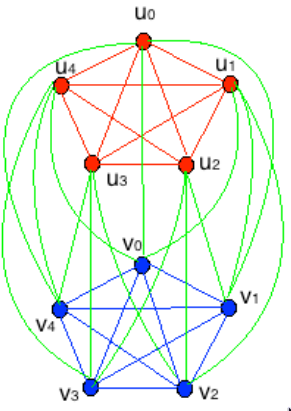
\includegraphics[width=0.3\linewidth]{images/WebCom.png}
    \caption{Esempio Web-Community con un solo nodo}
    \label{fig:wcexample}
\end{figure}

Se si osserva bene, comunque scegliamo un nodo $x$, l'\textit{unico} taglio minimo è del tipo $(\{x\}, V - \{x\})$, di dimensione 7. Infatti, se aggiungessimo un qualsiasi nodo insieme ad $x$ otterremmo un taglio di dimensione strettamente maggiore di 7.

Per esempio $12 = |(\{ u_0, u_1 \}, V - \{ u_0, u_1 \} )| >  |(\{ u_0 \}, V - \{ u_0 \} )| = 7$.

Se ci riveriamo alla definizione di cut-cumminity, non ha molto senso dire che il solo nodo $u_0$ compone una comunità, per questo è necessario dare una nuova definizione di comunità.

\subsection{Web-community}

Una web-community è un sottoinsieme dei nodi di un grafo, ciascuno dei quali ha più vicini fra i nodi del sottoinsieme che fra quelli esterni ad esso.

\begin{definizione}[Strong Web-community]
    Dato un grafo $G = (V, E)$, il sottoinsieme $C \subset V$ è una \textbf{strong web-community} se $C \neq \emptyset$ e
    \[
    \forall u \in C: |N(u) \cap C| > |N(u) \setminus C| = |N(u) \cap (V - C)|
    \]
    Alternativamente è comodo guardare alla precedente proprietà come il fatto che almeno la metà dei vicini di $u$ è all'interno di $C$.
    \[|N(u)| =  |N(u) \cap C| + |N(u) \setminus C| \implies  |N(u) \setminus C| = |N(u)| - |N(u) \cap C|\]
    Quindi, 
    \begin{align*}
        &\quad\quad\quad |N(u) \cap C| > |N(u) \setminus C| \\ 
        &\iff |N(u) \cap C| > |N(u)| - |N(u) \cap C| \\
        &\iff 2|N(u) \cap C| > |N(u)|\\ 
        &\iff \frac{|N(u) \cap C|}{|N(u)|} > \frac{1}{2}
    \end{align*}
\end{definizione}

\begin{definizione}[Weak Web-community]
    Dato un grafo $G = (V, E)$, il sottoinsieme $C \subset V$ è una \textbf{weak web-community} se $C \neq \emptyset$ e
    \[
    \forall u \in C: |N(u) \cap C| \geq |N(u) \setminus C| = |N(u) \cap (V - C)|
    \]
    Alternativamente è comodo guardare alla precedente proprietà come il fatto che almeno la metà dei vicini di $u$ è all'interno di $C$.
    \[|N(u)| =  |N(u) \cap C| + |N(u) \setminus C| \implies  |N(u) \setminus C| = |N(u)| - |N(u) \cap C|\]
    Quindi, 
    \begin{align*}
        &\quad\quad\quad |N(u) \cap C| \geq |N(u) \setminus C| \\ 
        &\iff |N(u) \cap C| \geq |N(u)| - |N(u) \cap C| \\
        &\iff 2|N(u) \cap C| \geq |N(u)|\\ 
        &\iff \frac{|N(u) \cap C|}{|N(u)|} \geq \frac{1}{2}
    \end{align*}
\end{definizione}

Queste definizioni possono essere generalizzate, richiedendo che:
\[
\frac{|N(u) \cap C|}{|N(u)|} > \alpha\ (\geq \alpha) \text{, per qualche costante } \alpha \in [0, 1]
\]

\newpage
\subsection{Relazione tra Cut e Web-communities}

\begin{teorema}[Relazione tra Cut e Web-communities]
    Sia $G = (V, E)$ un grafo; se $C \subset V$ è una cut-community per $G$ tale che $|C| > 1$. Allora, $C$ è una weak web-community per $G$.
\end{teorema}

\begin{proof}
    Supponiamo per assurdo che $C$ non sia una weak web-community. Allora, esiste un nodo $u \in C$ tale che $|N(u) \cap C| < |N(u) \setminus C|$. Poiché $|C| > 1$, allora esiste in $C$ un nodo $v$ distinto da $u$: ossia, $C \setminus \{u\} \neq \emptyset$.
    Inoltre
    \begin{align*}
        \underbrace{\vert (C \setminus \lbrace u \rbrace , (V \setminus C) \cup \lbrace u \rbrace ) \vert}_{\text{taglio indotto da} C' = C \setminus\{u\}}
        &= \vert (C, V \setminus C) \vert + \underbrace{\vert N(u) \cap C \vert - \vert N(u) \setminus C \vert}_{< 1 \text{, per ipotesi, } |N(u) \cap C| < |N(u) \setminus C|}\\
        &< \vert (C, V \setminus C) \vert
    \end{align*}
    Ponendo $C' = C \setminus \{u\}$ abbiamo trovato che il taglio indotto da $C'$ è \textbf{minore} del taglio indotto da $C$, e questo è assurdo in quanto essendo $C$ per ipotesi una cut-community deve essere vero che $(C, V \setminus C)$ è un taglio minimo di $G$. Perciò necessariamente è falsa l'ipotesi che $C$ non sia una weak web-community.
\end{proof}

Anche se esiste un algoritmo polinomiale che decide se un grafo è partizionabile in cut-community, non ne conosciamo uno che decida in tempo polinomiale se un grafo è partizionabile in web-communities.

Infatti, sappiamo trovare due cut-communities $C$, $V \setminus C$ che generino un taglio minimo, ma non sappiamo garantire che $|C| > 1$ e $|V \setminus C| > 1$. Infatti, osservando la \autoref{fig:wcexample}, $C = \{u_0\}$ è una cut-community, ma non è una web-community in quanto $u_0$ ha, ovviamente, più vicini in $V \setminus C$ che in $C$.

In realtà, non solo non conosciamo un algoritmo che possa farlo in tempo polinomiale, ma è possibile dimostrare che tale problema è \textbf{NP-completo}.

\subsection{Strong Web-Communities Partitiong (SWCP)}

Definiamo ora il problema decisionale \textbf{Strong Web-Communities Partitioning (SWCP)}. Dato un grafo $G = (V, E)$, decidere se esiste un sottoinsieme (proprio e non vuoto) $C$ di $V$ tale che $C$ e $V \setminus C$ sono due strong web-communities.

\begin{lemma}\label{lemma:swcp}
    Se $G=(V, E)$ è partizionabile in due strong web-communities e esistono $x, y, z \in V$ tali che $N(x) = \{y, z\}$ (ossia $x$ ha grado 2 in $G$), \textit{allora} per ogni $C \subset V$ tale che $C$ e $V \setminus C$ sono entrmabi due strong web-communities e i tre vertici $x, y, z \in C$ oppure $x, y, z \in V \setminus C$.
\end{lemma}
    In altre parole, Il lemma afferma che, in questa situazione, non è possibile che $y$ e $z$ si trovino in due community diverse: se il grafo è davvero partizionabile in due strong web-communities, allora i tre nodi $x,y,z$ devono stare tutti e tre nella stessa parte (tutti in $C$ oppure in $V \setminus C$.
\begin{proof}
    Sia $C \subset V$ tale che $C$ e $V \setminus C = \overline{C}$ sono due strong web-communities. Senza perdita di generalità, assumiamo che $x \in C$.
    \begin{itemize}
        \item Per assurdo, supponiamo che $y, z \in \overline{C}$, allora 
        \[
        |N(x) \cap C| = 0 < |N(x) \cap \overline{C}| = 2
        \]
        Per la definizione di strong web-community, ogni nodo appartenente a $C$ deve avere più connessioni dentro $C$ che fuori. Ma qui $x$ ha 0 dentro e 2 fuori, quindi $C$ non può essere una strong web-community.
        \item Per assurdo, supponiamo che $y \in C$ e $z \in \overline{C}$, allora
        \[
        |N(x) \cap C| = 1 = |N(x) \cap \overline{C}|
        \]
        La condizione di strong web-community richiede una disuguaglianza stretta (più collegamenti interni che esterni). Quindi anche qui la condizione è violata.
        \item Se invece $x \in V \setminus C$ e uno dei vicini fosse in $C$, si avrebbe lo stesso ragionamento inverso (stessi casi di sopra).
    \end{itemize}
    In conclusione, in tutti i casi verrebbe contraddetta l'ipotesi che $C$ e $V \setminus C$ sono due strong web-communities.
\end{proof}

\begin{teorema}
    SWCP è NP-completo.
\end{teorema}

\begin{proof}
    Innanzitutto dobbiamo verificare che il problema è \textbf{NP}: un certificato è un sottoinsieme $C \subset V$, e verificare che $C$ e $V \setminus C$ sono strong web-communities richiede tempo polinomiale in $|G|$. Quindi il problema è \textbf{NP}. Dobbiamo ora dimostrarne la completezza, riducendo a 3SAT.

    Siano:
    \begin{itemize}
        \item $X = \{x_1, \dots, x_n\}$ l'insieme delle variabili,
        \item $f = c_1 \land c_2 \land \dots \land c_m$ con $c_j = l_1 \lor l_2 \lor l_3$, 
        \item $l_{jh} \in X$ oppure $\lnot l_{jh}$ per $j = 1, \dots, m$ e $h = 1, 2, 3$.
    \end{itemize}

    Costruiamo ora un grafo costituito da due nodi "specializzati" $T$ e $F$ che potranno appartenere alla stessa comunità $C$ se e soltanto se $C = V$ (e quindi $C$ non è una comunità, poiché non è contenuta propriamente in $V$).

    In altre parole, l'insieme dei nodi $V$ contiene i nodi $T$ e $F$, che rappresenteranno le assegnazioni \texttt{true} e \texttt{false}.
    Questi due nodi sono posizionati nel grafo in modo tale che essi dovranno necessariamente appartenere a due comunità differenti affinché $G$ sia partizionabile in due strong web-community

    Per ogni variabile $x_i \in X$ definiamo il \textbf{gadget variabile} nel seguente modo:
    \begin{itemize}
        \item Inseriamo in $V$ i nodi $x_i, \lnot x_i(w_i), y_i, z_i, t_i, f_i$,
        \item Inseriamo in $E$ gli archi $(x_i,y_i), (x_i,z_i), (y_i,t_i), (t_i,T), (\lnot x_i, z_i), (\lnot x_i, y_i), (z_i, f_i), (f_i, F)$,
        \item Infine, inseriamo tanti nodi senza nome, collegati a $x_i$ e $\lnot x_i$ quante sono le clausole che contengono la variabile $x_i$ e $\lnot x_i$ più uno (come mostrato in \autoref{fig:gadget}).
    \end{itemize}
        \newpage
        \begin{figure}[ht!]
            \centering
            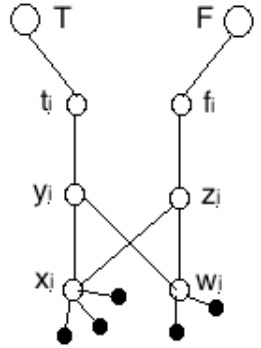
\includegraphics[width=0.2\linewidth]{images/gadgetxi.png}
            \caption{Gadget associato alla variabile $x_i$}
            \label{fig:gadget}
        \end{figure}
    Osserviamo che se $T$ ed $F$ appartengono a due comunità differenti, allora anche $x_i$ ed $\lnot x_i$ apparterranno a due comunità differenti. Infatti, senza perdita di generalità poniamo $T \in C$ e $F \in \overline{C} = V \setminus C$:
    poiché $t_i$ e $f_i$ hanno entrambi grado 2, per il \autoref{lemma:swcp} deve necessariamente essere vero che $t_i, y_i \in C$ e $f_i, z_i \in \overline{C}$. 

    Poiché $y_i$ ha grado 3, allora almeno uno tra $x_i$ e $\lnot x_i$ deve appartene a $C$.
    Stessa cosa per $z_i$, poiché ha grado 3 allora almeno uno tra $x_i$ e $\lnot x_i$ deve appartene a $\overline{C}$.

    Poiché $y_i$ e $z_i$ non devono poter essere raggiungibili (altrimenti apparterrebbero alla stessa comunità), allora possiamo dire che o $x_i$ appartiene e $C$ e $\lnot x_i$ a $\overline{C}$, oppure viceversa.

    Infine, per le osservazioni fatte sopra, anche ciascun nodo senza nome deve essere contenuto nella stessa comunità che contiene il padre.

    Continuando, per ogni clausola $c_j$ di $f$, definiamo un \textbf{gadget clausola} come segue:
    \begin{enumerate}
        \item Inseriamo in $V$ un nodo $c_j$ e un nodo per ognuno dei suoi letterali $l_{j1}, l_{j2}, l_{j3}$.
        \item In $E$ inseriamo gli archi da $c_j$ verso $l_{j1}, l_{j2}, l_{j3}$, e dai nodi $l_{j1}, l_{j2}, l_{j3}$ verso il nodo $T$.
        \item Infine, aggiungiamo in $E$ un arco da $c_j$ verso ognuno dei letterali che lo compongono: se in $c_j = x_1 \lor \lnot x_2 \lor x_3$ (\autoref{fig:ex_clausola}) allora inseriamo gli archi $(c_j, x_1), (c_j, \lnot x_2), (c_j, x_3)$.
    \end{enumerate}

    \begin{figure}
        \centering
        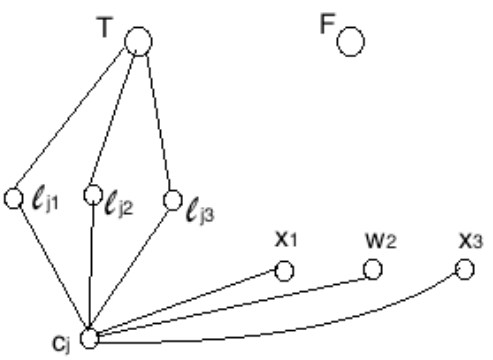
\includegraphics[width=0.3\linewidth]{images/ex_clausola.png}
        \caption{Clausola $c_j$}
        \label{fig:ex_clausola}
    \end{figure}

     Notiamo che sempre per il \autoref{lemma:swcp}, dato che $l_{j1},l_{j2},l_{j3}$ hanno tutti grado 2, allora se $G$ è partizionabile in due strong web-community, certamente sia $l_{j1},l_{j2},l_{j3}$ che $c_j$ devono essere nella stessa comunità a cui appartiene $T$.

     Dalla costruzione appena fatta emerge che quindi $c_j$ deve appartenere alla stessa comunità a cui appartiene $T$, e per rendere ciò possibile \text{almeno} uno dei letterali che lo compongono deve appartenere alla stessa comunità. Nell'esempio nella \autoref{fig:ex_clausola}, almeno uno tra $x_1, \lnot x_2, x_3$ deve essere contenuto in $C$, altrimenti $c_j$ avrebbe tanti vicini in $C$ quanti in $V \setminus C$.

    \begin{figure}[ht!]
        \centering
        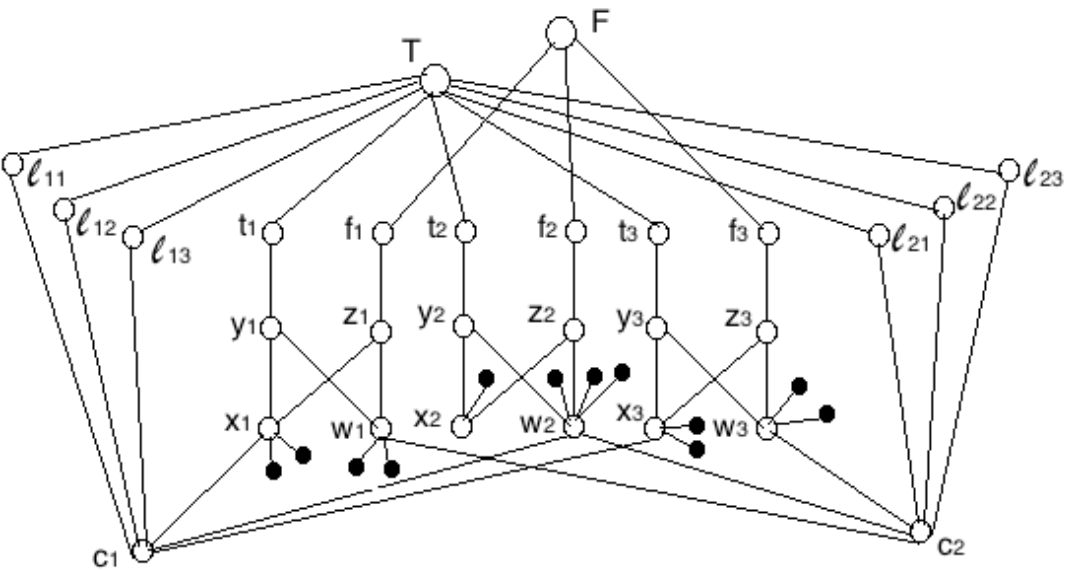
\includegraphics[width=0.5\linewidth]{images/funzione_completa.png}
        \caption{
            $f(x_1, x_2, x_3) = c_1 \land c_2 = (x_1 \lor \lnot x_2 \lor \lnot x_3) \land (\lnot x_1 \lor \lnot x_2 \lor \lnot x_3)$
            }
    \end{figure}

    Iniziamo col dimostrare che $T$ ed $F$ devono necessariamente appartenere a due comunità differenti, e questo verrà dimostrato dimostrando che se $T$ ed $F$ appartengono alla stessa comunità $C$ allora $C \equiv V$
    \[
    T, F \in C \Leftrightarrow C \equiv V
    \]
    Iniziamo con l'osservare che se $T,F$ appartengono alla stessa comunità $C$ allora anche i nodi $y_i$ e $z_i$ appartengono a $C$, per ogni $i = 1, 2, \dots, n$.
    
    Consideriamo il letterale $x_i$ che è contenuto in $k$ clausole del tipo $c_j$.
    Poiché ognuna di queste clausole sono per costruzione nella stessa comunità di $T$ (e quindi in $C$) e poiché $x_i$ ha altri due suoi vicini $y_i, z_i$ in $C$, risulterà che più della metà dei suoi vicini sono in $C$. Infatti risulta che $x_i$ ha esattamente $k+2$ vicini in $C$ più altri $k+1$ nodi senza nome.
    Perciò, dovunque inseriamo qui $k+1$ nodi senza nome, per forza $x_i$ deve stare in $C$. Stesso ragionamento per $\lnot x_i$.
    
    \begin{figure}[ht!]
        \centering
        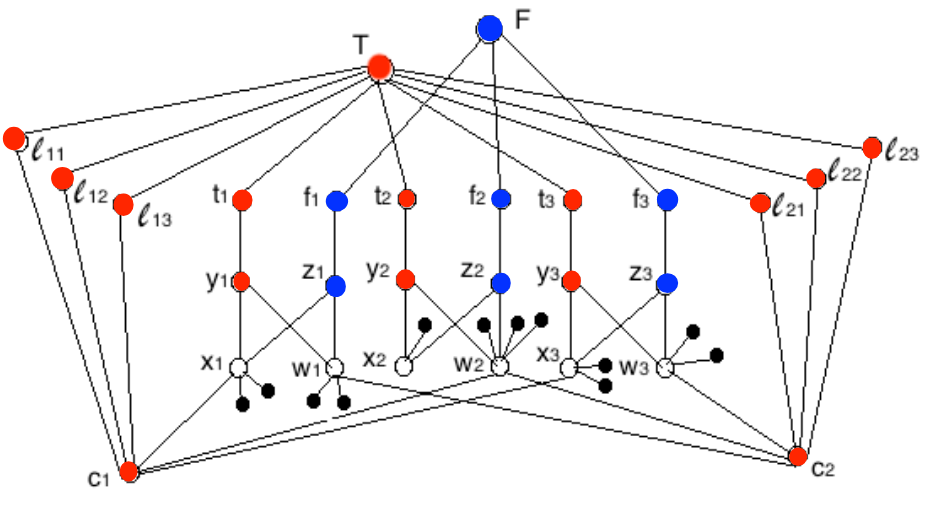
\includegraphics[width=0.5\linewidth]{images/funzione_completa_col.png}
        \caption{}
        \label{fig:funzione_completa_col}
    \end{figure}

    Per comprendere meglio il concetto, osserviamo la \autoref{fig:funzione_completa_col}. Se $T$ e $F$ sono due diverse comunità, allora, per ogni $c_j$ i nodi $c_j, l_{j1}, l_{j2}, l_{j3}$ sono nella stessa comunità di $T$ (nodi in rosso). Per ogni variabile $x_i$, i nodi $t_i$ e $y_i$ sono con $T$ (rossi) e i nodi $f_i$ e $z_i$ sono con $F$ (blu).
    Allora, dobbiamo "colorare" i nodi $x_i$ e $\lnot x_i (w_i)$ per ogni variabile $x_i$, in modo che l'insieme dei nodi rossi e l'insieme dei nodi blu siano strong web-communities.

    Riassumendo, $G$ è partizionabile in due strong web-communities $C$ e $V \setminus C$ se e soltanto se $T$ e $F$ \textbf{non} sono entrambi in $C$ e non sono entrambi in $V \setminus C$, ovvero appartengono a comunità diverse.

    Quindi, affinché $T \in C$ e $F \in V \setminus C$, devono valere le seguenti due proprietà:
    \begin{enumerate}
        \item Per ogni variabile $x_i \in X$, \textbf{esattamente uno dei nodi $x_i$ e $\lnot x_i$ deve essere contenuto in $C$ e esattamente uno dei nodi $x_i$ e $\lnot x_i$ deve essere contenuto in $V \setminus C$}. 
        
        Allora, ogni partizione in $G$ in due strong web communities corrisponde ad una assegnazione di verità $a$ per $X$ che soddisfa $f$. 

        \[
            a(x_i) = 
            \begin{cases}
                \texttt{true}& if\  x_i \in C\\
                \texttt{false} & if\ x_i \in V \setminus C
            \end{cases}
        \]
        dove $C$ è la comunità a cui appartiene $T$.
        
        Viceversa, se esiste un'assegnazione $a: X \rightarrow \lbrace \texttt{true}, \texttt{false} \rbrace$ che soddisfa $f$, allora è possibile ricavare una partizione di $G$ in due web-communities.

        \item Per ogni clausola $c_j$, il nodo $c_j$ \textbf{deve} appartenere a $C$ (che contiene $T$), e perché questo sia possibile \textbf{è necessario che almeno uno dei nodi nei gadget variabile collegato a $c_j$ sia contenuto in $C$, ossia, uno dei nodi corrispondenti a un letterale nella clausola $c_j$ deve essere contenuto in $C$}.

        Innanzitutto poniamo $T$ in $C$ ed $F$ in $V \setminus C$. Dopodiché, dato che $a$ soddisfa $f$, allora inseriamo in $C$ tutti i nodi clausola $c_j$ e i rispettivi $l_{j1}, l_{j2}, l_{j3}$. Infine, per ogni $i$, inseriamo in $C$ i seguenti nodi:
        \begin{itemize}
            \item  se $a(x_i) = \texttt{true}$, inseriamo $x_i$, i suoi nodi senza nomi, e i nodi $y_i, t_i$.
            \item se $a(x_i) = \texttt{false}$, inseriamo $\overline{x_i}$, i suoi nodi senza nomi, e i nodi $y_i, t_i$.
        \end{itemize}
    \end{enumerate}
        
    Le due comunità risultanti saranno due cut-communites.
\end{proof}

\newpage

\section{Partizionare un grafo in comunità:
approccio euristico}

In questa parte verranno mostrate due famiglie approcci che dal punto di vista euristico riescono a partizionare un grafo in comunità accettabili, ovvero in gruppi di nodi abbastanza coesi tra di loro.

Più precisamente i due metodi si dividono in:
\begin{itemize}
    \item \textbf{Metodi partitivi}, in cui si parte considerando l'intero grafo come unica grande comunità, e la si inizia a disconnettere (rimuovendo archi) finché non si otterranno due comunità distinte e coese. Se si desidera ottenere una \textbf{granularità} maggiore basta iterare il metodo sui sotto grafi ottenuti.
    \item \textbf{Metodi agglomerativi}, in cui si parte considerando ogni singolo nodo una comunità, e man mano si aggiungono gli archi del grafo finché non si otterranno un numero di comunità desiderato con un livello di coesione accettabile.
\end{itemize}

\subsection{Betwenness di un Arco}

Vediamo ora un particolare criterio per rimuovere gli archi in un metodo partitivo. In particolare, il criterio che andremo a vedere si basa sul concetto di \textbf{betwenness di un arco}, che a sua volta si basa sui concetti di bridge e local bridge. Ricordiamo che un bridge (per definizione), connette due regioni del grafo che altrimenti risulterebbero non connesse. Mentre un bridge, connette due regioni che, senza di esso, sarebbero connesse in modo meno efficiente. Possiamo quindi dire che bridges e local bridges connettono regioni che, senza di loro, avrebbero difficoltà ad interagire. Inoltre, sappiamo che questi arco sono weak ties, quindi gli archi che rimangono dopo la loro rimozione sono gli strong ties - quelli delle relazioni forti.

Quindi l'idea alla base di questo criterio è la seguente: rimuovendo bridges e local bridges il grafo viene partizionato in componenti che bene pososno essere considerate comunità.

Consideriamo la rete in \autoref{fig:controesempio_weak_strong}. Non è presente nessun local bridge, ma è facile osservare che esitono due comunità (cerchiate in rosso).

\begin{figure}
    \centering
    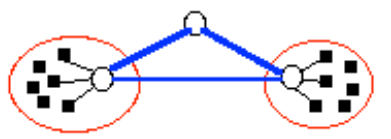
\includegraphics[width=0.5\linewidth]{images/BTcontroesempio.png}
    \caption{Controesempio weak/strong ties}
    \label{fig:controesempio_weak_strong}
\end{figure}

Al fine di definire il metodo partitivo, è necessario definire il concetto di betwenness di un arco. Essa è basato sulla nozione di traffico (o flusso) di informazioni che passa attraverso gli archi.

Possiamo considerare come "nuovi archi ponte" tutti quegli archi attraverso i quali passa una grande quantità di flusso, e che se rimossi rendono più difficile la comunicazione tra due comunità.

Secondo questo criterio possiamo rimuovere gli archi sui quali passa maggior flusso, finché non otterremo un partizionamento accettabile della rete.


Sia $G=(V, E)$ non orientato.
\begin{definizione}
    Definiamo con $\sigma_{st}(u,v)$ il numero di \textbf{shortest-paths} (\textbf{camminimi minimi}) $\pi^\star(s,t)$  tra $s$ e $t$ che passano per l'arco $(u,v)$.
    \[
    \sigma_{st} = |\{\pi^\star(s,t)\}|
    \]
\end{definizione}

\begin{definizione}[Betweeness Relativa]
    Definiamo poi con $b_{st}(u,v)$ la \textbf{betweennes relativa} all'arco $(u,v)$ \textbf{rispetto alla coppia} $s,t$ come la \textbf{frazione} di shortest path $\pi^\star(s,t)$ che passano per l'arco $(u,v)$.
    \[
        b_{st}(u,v) = \frac{\sigma_{st}(u,v)}{\sigma_{st}}
    \]
\end{definizione}

\begin{definizione}[Betweeness Totale]
    Definiamo la \textbf{betweenness} $b(u,v)$ di un arco $(u,v)$ come la \textbf{semi-somma} di tutte le betweenness relative $b_{st}(u,v)$, per ogni coppia di nodi $s,t$
    \[
    b(u,v) = \frac{1}{2} \sum_{(s,t) \in \binom{V}{2}} b_{st}(u,v)
    \]
Notare che il fattore $1/2$ è necessario per evitare di contare le ripetizioni, del tipo $b_{st}(u,v)$ e $b_{ts}(u,v)$.
\end{definizione}

Analogamente alla \textbf{edge-betweenness} si può definire una \textbf{node-betweenness}, seguendo la stessa definizione.

\subsection{Metodo di Girvan-Newman}

Il metodo di Girvan-Newman è un metodo partitivo che si basa sulla betweenness. Si inizia considerando l'intero grafo coem un'unica grande comunità, poi si calcola l'arco di betweenness massima e si rimuove: se il grafo residuo è non connesso allroa è stata ottenuta una prima partzione in comunità. Il procedimento viene poi iterato calcolando gli archi di betweenness massima nel grafo rimanente e rimuovendoli. Il procedimento ha termine quando si è ottenuto un livello di granularità ritenuto adeguato.

Lo schema dell'algoritmo per il calcolo delle betweenness degli archi è il seguente:

Per ogni $s \in V$, si eseguono i seguenti tre passi:
\begin{enumerate}
    \item Calcola il sottografo $T(s)$ degli shortest path uscenti da $s$ mediante una BFS.
    \item Mediante una visita \textbf{top-down} di $T(s)$, per ogni nodo $V \in V$ calcola $\sigma_{sv}$ (numero di shortest path da $s$ a $v$).
    \item Mediante una visita \textbf{bottom-up} di $T(s)$, e usando quanto calcolato al punto (2), per ogni $(u, v) \in T(s)$ calcola 
    \[
        b_s(u,v) = \sum_{t \in V \setminus \{s\}} b_{st}(u, v)    
    \]
\end{enumerate}
Infine, per ogni arco $(u,v) \in E$, si calcola 
\[
    b(u,v) = \frac{1}{2} \sum_{(s,t) \in \binom{V}{2}} b_{st}(u,v)
\]

Vediamo meglio nel dettaglio come funzionano le fasi (1), (2) e (3).

\subsubsection{Fase 1}
Per calcolare $T(s)$ basta effettuare una visita in ampiezza \textbf{BFS} opportunamente modificata.

Definiamo con $L_h$ l'insieme di tutti i nodi a distanza $h$ dalla sorgente $s$.
Diremo che un nodo $v$ si trova al \textbf{livello} $h$ se $v \in L_h$.

Se un nodo $v$ si trova al livello $h$, allora certamente \textbf{tutti} i cammini minimi da $s$ a $v$ termineranno con archi che partono da $L_{h-1}$.
Perciò, tutti gli archi $(u,v)$ con $u \in L_{h-1}$ e $v \in L_h$ faranno parte di $T(s)$.

Perciò possiamo calcolare $T(s)$ nella seguente maniera (\autoref{fig:fase1}):

\begin{enumerate}
    \item Poniamo inizialmente $L_0 = \lbrace s \rbrace$ e $T(s) = \emptyset$.
    \item Per ogni $h \geq 0$ calcoliamo $L_{h+1}$ come tutti quei nodi \textbf{fuori} $L_0 \cup L_1 \cup \dots \cup L_h$ tali che hanno almeno un vicino in $v \in L_h$, ovvero come
    \[
    L_{h+1} \equiv \{ v \in V \setminus (L_0 \cup L_1 \cup \dots \cup L_h)\ |\ \exists u \in L_h : (u,v) \in E  \}
    \]
    \item Calcolato $L_{h+1}$ poniamo $T(s)$ come 
    \[
    T(s) = T(s) \cup \{ (u,v) \in E\ |\ u \in L_h \land v \in L_{h+1} \}
    \]
\end{enumerate}
    \begin{figure}[ht!]
        \centering
        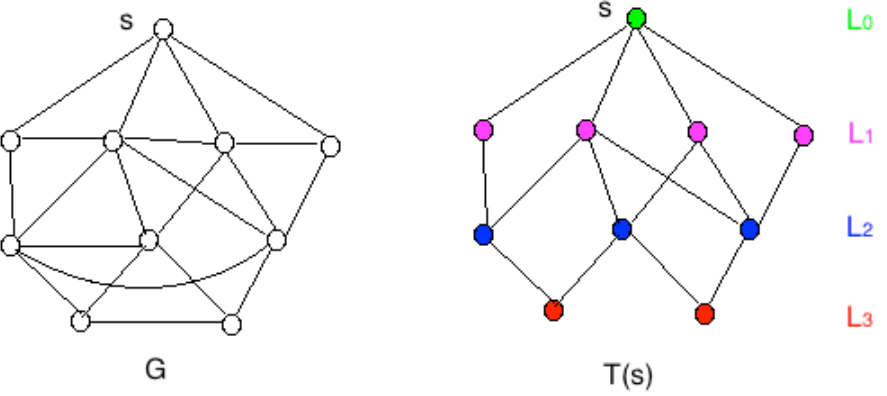
\includegraphics[width=1\linewidth]{images/fase1GN.png}
        \caption{Costruzione sottografo cammini minimi}
        \label{fig:fase1}
    \end{figure}

\newpage
\subsubsection{Fase 2}

Calcolato $T(s)$, possiamo sfruttarlo per calcolare, per ogni $v \in V$, la quantità $\sigma_{sv}$, ovvero il numero di cammini minimi che vanno da $s$ a $v$.

In altre parole, il numero numero di shortes paths dalla radice $s$ a un nodo $v \in L_h$ è pari alla somma dei numero dei percorsi da $s$ a un qualunque "padre" di $v$.

Iniziamo osservando che per ogni nodo $v$ nel livello 1, il numero di cammini minimi sarà pari ad 1 (perché $v$ è diretto vicino di $s$).

Invece al livello 2, il numero di cammini minimi di un generico nodo $v \in L_2$ è pari alla somma di tutti i $\sigma_{su}$, tali che esiste $(u,v)$ con $u \in L_1$. Più in generale, per ogni $v \in L_h$, possiamo calcolare $\sigma_{sv}$ con la seguente formula ricorsiva
\[
	\sigma_{sv} =\begin{cases}
    1  & \text{if } h = 1\\
	\sum\limits_{(u,v) \in E\ |\ u \in L_{h-1}} \sigma_{su}  & \text{if }h > 1
	\end{cases} 
\]

\begin{figure}[ht!]
    \centering
    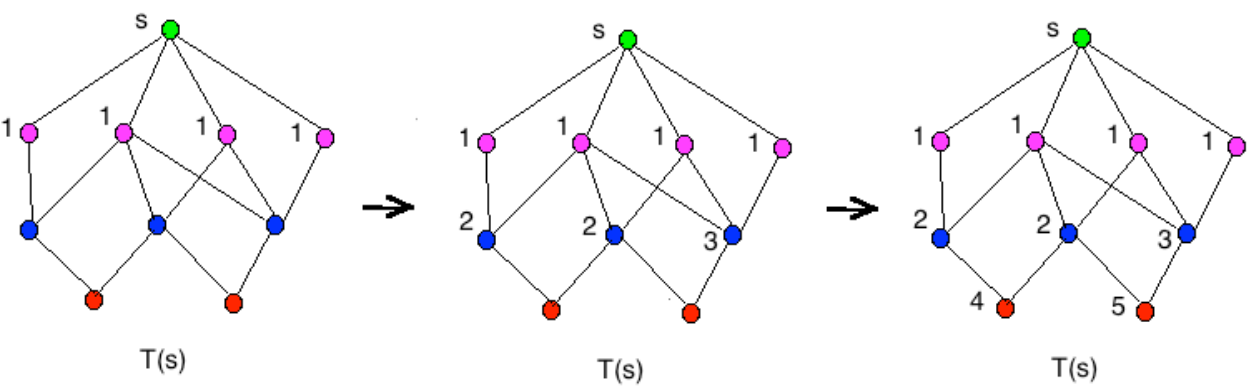
\includegraphics[width=0.8\linewidth]{images/fase_2.png}
    \caption{Calcolo dei cammini minimi in $T(s)$}
    \label{fig:fase2}
\end{figure}

\subsubsection{Fase 3}

Nella terza fase dobbiamo calcolare per ogni arco $(u,v) \in T(s)$ la quantità di flusso che ci passa sopra rispetto a $s$, ovvero 
\[
    b_s(u,v) = \sum_{t \in V \setminus \{ s \}} b_{st}(u,v)
\]
Per fare ciò in questo caso faremo una visita "bottom-up" di $T(s)$.

Sia $d$ il numero di livelli in $T(s)$, e consideriamo un arco $(y,x)$ con $y \in L_{d-1}$ e $x \in L_d$. 

Osserviamo che tutti gli shortest path che partono da $s$ e passano attraverso l'arco $(y,x)$ sono tutti shortest path che terminano in $x$.

Perciò il flusso che passa su $(y,x)$ rispetto a $s$ sarà pari al rapporto tra il numero di shortest path che vanno da $s$ a $y$ (ovvero $\sigma_{sy}$) e il numero complessivo di shortest path che vanno da $s$ ad $x$ (ovvero $\sigma_{sx}$).
\[
b_s(y,x) = \sum_{t \in V \setminus \{ s \}} b_{st}(y,x) = b_{sx}(y,x) = \frac{\sigma_{sx}(y,x)}{\sigma_{sx}} = \frac{\sigma_{sy}}{\sigma_{sx}}
\]
Analogamente possiamo applicare questo ragionamento per tutti gli archi che collegano nodi dell'ultimo livello, come mostrato in \autoref{fig:fase3_a}.

\newpage

\begin{figure}[ht!]
    \centering
    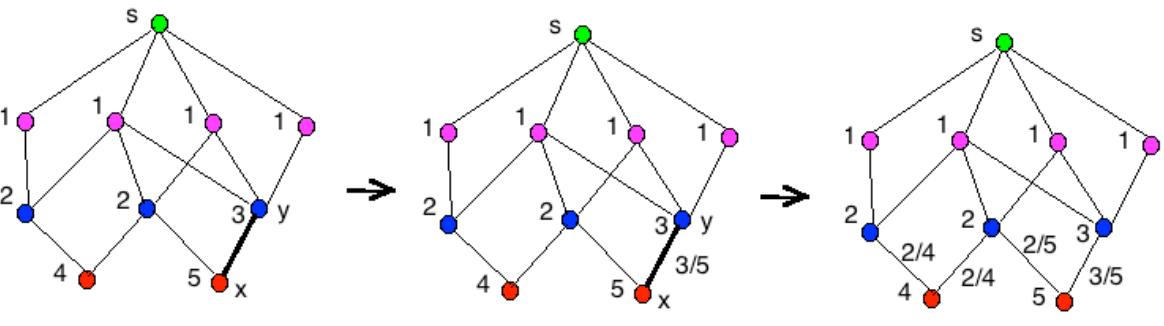
\includegraphics[width=0.8\linewidth]{images/fase3_a.png}
    \caption{Calcolo di $b_s(y,x)$}
    \label{fig:fase3_a}
\end{figure}

Adesso, saliamo di un livello, e consideriamo gli archi che entrano nel livello $L_{d-1}$.

Rifacendoci alla \autoref{fig:fase3_b}, consideriamo l'arco $(z, y)$, con $z \in L_{d-2}$ e $y \in L_{d-1}$.

\begin{figure}[ht!]
    \centering
    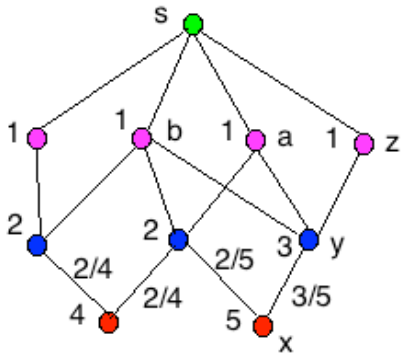
\includegraphics[width=0.3\linewidth]{images/fase3_b.png}
    \caption{Immagine in esempio}
    \label{fig:fase3_b}
\end{figure}

Osserviamo che tra tutti i cammini minimi che passano per l'arco $(z, y)$, una parte saranno cammini che termineranno in $y$, e una parte saranno cammini minimi che andranno ai nodi di livello inferiore.

Perciò la frazione di shortest path che, partendo da $s$, passano per $(z, y)$ è pari alla somma dei seguenti fattori:
\begin{itemize}
    \item La frazione degli shortest path da $s$ ad $y$, ovvero $\frac{\sigma_{sz}}{\sigma_{sy}}$. 
    \item Per ogni \textbf{diretto discendente} $x$ di $y$, una frazione $\frac{\sigma_{sz}}{\sigma_{sy}}$ della frazione di shortest path da $s$ ad $x$ che passano per l'arco $(y,x)$, ovvero 
    \[
    \frac{\sigma_{sz}}{\sigma_{sy}} \cdot \frac{\sigma_{sy}}{\sigma_{sx}} = \frac{\sigma_{sz}}{\sigma_{sx}}
    \]
\end{itemize}


Quindi, rifacendoci all'esempio, avremo che 
\[
b_s(z,y) = \frac{\sigma_{sz}}{\sigma_{sy}} + \frac{\sigma_{sz}}{\sigma_{sy}} \cdot \frac{\sigma_{sy}}{\sigma_{sx}} = \frac{1}{3} + \frac{1}{3}\cdot\frac{3}{5} = \frac{8}{15}
\]
Così facendo abbiamo definito un metodo "bottom-up" per il calcolo tutti i valori $b_s(u,v)$.

Infine, dopo l'esecuzione di queste 3 fasi, calcoliamo la betweenness finale come:
\[
    b(u,v) = \frac{1}{2} \sum_{s \in V} b_s(u,v)
\]

Notiamo che questa procedura permette di calcolare la betweennes degli archi in tempo \textbf{polinomiale} nella grandezza della rete (e non esponenziale).

Infatti la (1) è una semplice visita in ampiezza del grafo (e si può calcolare in tempo $O(|V| + |E|)$), la (2) è un'ulteriore visita in ampiezza di $T(s)$ (e si può calcolare ancora in tempo $O(|V| + |E|)$), e infine la (3) è nuovamente una visita in ampiezza, partendo però dal livello più basso (ancora una volta $O(|V| + |E|)$).

Dato che bisogna iterare questo procedimento per ogni nodo del grafo, e dato che nel caso peggiore abbiamo grafi molto densi con $\Theta(n^2)$ archi, la complessità temporale dell'esecuzione di questo algoritmo per il calcolo delle betweennes sarà $O(nm) \in O(n^3)$.

\section{Rilassare il Modello}

Nel modello teorico originale delle reti sociali, le relazioni venivano considerate in modo dicotomico: gli archi potevano essere \textit{strong ties} o \textit{weak ties}, e alcuni potevano essere \textit{bridge edges}. Tuttavia, questo approccio è troppo rigido per le reti reali, dove raramente esistono veri \textit{bridge edges} e la forza delle relazioni non è classificabile in modo netto.

Per rendere il modello più realistico, si introduce quindi una \textbf{rete pesata}:
\[
G = (V, E, w) \text{ dove } w : E \rightarrow \mathbb{N}
\]
ossia $w(u,v)$ rappresenta numericamente la \textit{forza} del legame tra due nodi.

Il concetto di \textit{bridge edge} viene sostituito dal \textbf{neighborhood overlap (NO)}, che misura la frazione di amici in comune tra due nodi:
\[
NO(u,v) = \frac{|N(u) \cap N(v)|}{|N(u) \cup N(v) - {u,v}|}
\]
Un \textit{local bridge} ha dunque $NO(u,v) = 0$.

Poiché nel modello classico la Strong Triadic Closure Property garantisce che i local bridge siano weak ties, ci si chiede se una relazione simile tra forza del legame e ruolo strutturale esista anche nel modello pesato.

A supporto di questa idea vi sono i risultati empirici di \textbf{Onnela et al. (2007)}, che analizzarono una grande rete telefonica reale. Essi costruirono un grafo dai dati delle chiamate e procedettero a rimuovere gli archi:

\begin{enumerate}
    \item prima rimuovendo quelli con \textbf{peso alto}, osservando che la rete rimaneva connessa a lungo;
    \item poi rimuovendo quelli con \textbf{peso basso} osservando la rete si disconnetteva rapidamente.
\end{enumerate}

Questi risultati suggeriscono che gli archi con peso basso svolgono un ruolo cruciale nel collegare comunità diverse e quindi hanno \textbf{basso neighborhood overlap}, analogamente ai weak ties del modello classico.

In sintesi, anche nel modello rilassato sembra esistere una correlazione empirica tra \textbf{bassa forza del legame} (peso) e \textbf{basso neighborhood overlap}, analoga alla relazione tra weak ties e local bridges.

\section{Conclusioni}

Ricapitolando, una rete sociale può essere vista come un insieme di gruppi 
densamente connessi tramite relazioni forti, mentre tali gruppi sono a loro volta 
collegati tra loro attraverso relazioni deboli.

Dal punto di vista sociale, l'appartenenza ad un gruppo porta numerosi vantaggi: 
più un individuo è ben inserito all'interno del proprio gruppo --- ovvero più gode 
della fiducia dei suoi vicini --- maggiori benefici ottiene. Contrariamente, 
l'esperimento di Granovetter mostra che è spesso altrettanto utile mantenere 
connessioni con individui appartenenti ad altri gruppi, poiché questo permette 
di accedere a nuove e potenzialmente vantaggiose fonti di informazione.

Queste osservazioni suggeriscono che i vantaggi di un nodo non dipendono solo 
dalla sua appartenenza ad una comunità, ma anche dalla sua posizione nella rete 
e dal grado di integrazione nel proprio gruppo. Per formalizzare questa idea 
introduciamo il concetto di \textbf{embeddedness} di un arco $(u,v)$, definito come 
la quantità di vicinato condiviso tra i due nodi:
\[
\text{Emb}(u,v) = |N(u) \cap N(v)|.
\]
Si osserva che un \textit{local bridge} è un arco con embeddedness pari a $0$.

Una embeddedness elevata indica che i due estremi dell'arco sono ben integrati 
nella stessa comunità. Analogamente, un nodo che presenta molti archi con alta 
embeddedness è un nodo fortemente inserito nel proprio gruppo.

Nell'esempio precedente, il nodo \texttt{A} risulta ben integrato nella sua 
comunità, in quanto occupa una posizione centrale: tutti i suoi archi hanno 
embeddedness elevata. Al contrario, il nodo \texttt{B} si trova in una posizione 
marginale, avendo pochi archi con embeddedness alta.



\chapter{Dinamiche nelle Reti - Processi di Diffusione}

Uno dei quesiti principali fin ora posti è cercare di capire come le scelte dei singoli individui sono influenzate dal comportamento degli altri individui. Quando si fa questo tipo di analisi si può considerare la rete sottostante in due differenti livelli di risoluzione: un livello in cui guardiamo la rete dall'alto e osserviamo il comportamento di gruppi di individui, e un livello più dettagliato in cui si considera la struttura della rete come grafo e si cerca di analizzare/intuire come i singoli individui sono influenzati dal loro diretto vicinato.

In questa parte verrà analizzato il secondo punto di vista, assumendo che i singoli individui abbiano solo una visione locale della rete, e non globale, e di conseguenza che prendano decisioni in base a ciò che osservano (ovvero in base al comportamento dei loro vicini). Questo framework è abbastanza ragionevole, in quanto è ragionevole pensare che una persona venga influenzata e cambi comportamento in base al gruppo in cui appartengono, ricevendo così benefici. Per esempio è conveniente che una persona adotti una nuova lingua perché la grande maggioranza delle persone con cui a che fare parlano tale lingua, fregandosene di quale sia la lingua più parlata in assoluto al livello globale.

Questi ragionamenti sono alla base del concetto di \textbf{omofilia}. Per omofilia da una parte si intende la capacità che ha un individuo di creare relazioni con altri individui che più gli assomigliano (riferendoci per esempio alla chiusura triadica), e dall'altra parte è la tendenza a cercare di assomigliare a chi li circonda in modo tale da trarne vantaggi. Per esempio in un contesto sociale reale le persone tendono a creare rapporti con altre persone che hanno stessi gusti e/o opinioni, d'altro canto però spesso per ridurre la tensione sociale si tende a scendere a compromessi adattandosi a ciò che vogliono gli altri.

\section{Coordination Game - Modello Lineare}

Come ogni altro argomento, partiamo da degli esempi reali, e proviamo in seguito a formalizzare un modello che descriva al meglio l'esempio studiato.
Iniziamo con parlare del \textit{processo di diffusione delle innovazioni}. Esso è stato studiato in sociologia già a partire dalla metà del secolo scorso. Ryan e Gross, hanno osservato il processo di adozione di nuovi semi ibridi di mais da parte di un gruppo di agricoltori di Iowa. Sebbene la maggior parte degli agricoltori veniva a conoscenza dei nuovi semi tramite
le comunicazioni dei venditori, a parte un numero limitato di agricoltori, la maggior parte degli agricoltori iniziava a usare i nuovi semi solo dopo aver osservato che un certo numero di vicini / conoscenti / amici li stava utilizzando.

Lo scopo quindi è di modellare un processo di diffusione in una rete. Per fare ciò bisogna innanzitutto definire delle regole in base alle quali un nodo decide di cambiare. Definiamo quindi un modello di decisioni \textbf{individuali}, ovvero non c'è una coalizione di gruppi di nodi per prendere collettivamente la stessa decisione, ma ciascun nodo decide per se stesso. Le scelte dei nodi, infatti, sono guidate da \textbf{motivazioni di puro interesse personale}.

Assumiamo quindi che, nella rete si sia stabilizzato una certo stato $B$, e che, ad un certo istante, alcuni individui cambino il loro stato in $A$. La domanda che ci poniamo ora è: \textit{in quali casi un individuo decide di cambiare il proprio stato da $B$ a $A$?} (Inoltre, assumiamo che una volta passato da $B$ a $A$, non si può più tornare indietro).

Il modello che stiamo considerando si basa sul concetto di \textbf{Network Coordination Game}.

\begin{definizione}[Modello del Processo di Diffusione]
    Sia $G = (V, E, \{A, B\})$ la nostra rete, e consideriamo l'arco $(u, v) \in E$. A ciascun stato $A, B$, associamo un beneficio, rispettivamente $a, b$ (\autoref{tab:benefici})

    
    \begin{table}[h!]
        \centering
        \begin{tabular}{|c|c|c|}
        \hline
        \diagbox{$u$}{$v$} & A & B \\ \hline
        A & \rule{0pt}{14pt}$a,a$ & \rule{0pt}{14pt}$0,0$ \\ \hline
        B & \rule{0pt}{14pt}$0,0$ & \rule{0pt}{14pt}$b,b$ \\ \hline
        \end{tabular}
        \caption{Tabella dei benefici}
        \label{tab:benefici}
    \end{table}
    \begin{itemize}
        \item Se $u$ e $v$ adottano entrambi lo stato $A$, allora entrambi hanno un beneficio pari ad $a$;
        \item Se $u$ e $v$ adottano entrambi lo stato $B$, allora entrambi hanno un beneficio pari ad $b$;
        \item Altrimenti, nessuno dei due ha alcun beneficio.
    \end{itemize}
\end{definizione}

Ovviamente il nodo $v$ gioca una copia del coordination game su ognuno dei suoi archi incidenti, perciò il suo guadagno sarà la somma di tutti i guadagni su ogni arco.
Andiamo ora ad analizzare quando al nodo $v$ conviene adottare lo stato $A$ oppure no, sapendo che parte dallo stato $B$.

Definiamo con $n_A$ ed $n_B$ il numero dei suoi vicini rispettivamente negli stati $A$ e $B$. Intuitivamente viene da pensare che $v$ agisce nei seguenti modi:
\begin{itemize}
    \item Se $bn_B > an_A$ allora gli conviene rimanere in $B$.
    \item Se $an_A > bn_B$ allora gli conviene adottare $A$.
\end{itemize}

Assumiamo che nel caso di parità di guadagno venga comunque preferita l'innovazione $A$ anziché rimanere nello stato attuale. Perciò si adotta lo stato $A$ se $an_A \geq bn_B$.

Supponiamo che una porzione $p$ dei vicini di $v$ sia nello stato $A$, e che una frazione $1-p$ sia nello stato $B$
\begin{align*}
    p &= \frac{n_A}{| N(v) |}\\
    1-p &= \frac{n_B}{| N(v) |} = \frac{| N(v) | - n_A}{| N(v) |}
\end{align*}
Perciò possiamo dire che a $v$ conviene cambiare stato se
\begin{align*}
    n_A a &\geq n_B b\\
    (| N(v) | \cdot p) a &\geq (| N(v) | \cdot (1-p)) b\\
    p a &\geq (1-p)b\\
    p &\geq \frac{b}{a+b}
\end{align*}

\begin{definizione}[Soglia di Adozione]
Definiamo la soglia di adozione
\[
q = \frac{b}{a+b}
\]
la frazione minima dei vicini di $v$ che devono essere nello stato $A$ per rendere l'adozione di $A$ conveniente rispetto a $B$.
\end{definizione}

\begin{itemize}
    \item Se $a >> b$, allora $q$ è molto piccolo, quindi occorrono pochi vicini nello stato $A$ per indurre un nodo a cambiare stato (questo accade quando $A$ è migliore dello stato $B$).
    \item Se $a = b$, occorrono almeno la metà dei vicini nello stato $A$ per indurre un nodo a cambiare stato.
    \item Se $a << b$, allora $q$ è molto alto, quindi occorrono molti più vicini nello stato $A$ per indurre un nodo a cambiare stato (questo accade quando $A$ è peggiore dello stato $B$).
\end{itemize}

\section{Comportamento a Cascata}

Dobbiamo ora capire se esistono delle configurazioni di equilibrio, ovvero una configurazione del grafo nella quale non c'è più la transizione dallo stato $B$ allo stato $A$. Osserviamo che esistono 2 tipologie di configurazioni di equilibrio:
\begin{enumerate}
    \item Quando $A$ non è stato introdotto nella rete, cosicché tutti i nodi rimangono nello stato $B$.
    \item Quando, dopo che $A$ è stato introdotto nella rete, tutti i nodi sono passati nello stato $A$.
\end{enumerate}

Ovviamente la seconda configurazione è più interessante da studiare, in quanto bisogna capire quando termina il processo di diffusione, se lo stato $A$ riesce a raggiungere tutti i nodi, oppure, talvolta, la diffusione si blocca (e perché si blocca) ancor prima di aver raggiunto tutti i nodi, e porta la rete in configurazioni intermedie.

%\newpage

\subsection{Esempio 1}

Consideriamo il processo di diffusione dello stato $A$ nella rete in \autoref{fig:Diff_ex1}. Lo stato $A$ è stato forzato all'inizio sui nodi $v$ e $w$. Poniamo i guadagni $a = 3$ e $b = 2$, ottenendo come soglia di adozione $q = \frac{2}{5}$, ossia, almeno $q$ vicini di un nodo devono trovarsi nello stato $A$ affinché venga adottato dal nodo stesso. Nell'esempio in questione, i nodi $r$ e $t$ passeranno allo stato $A$, in quanto hanno entrambi $\frac{2}{3} > \frac{2}{5}$ vicino nello stato $A$. Successivamente, anche $s$ e $u$, ottenendo così una diffusione totale dello stato $A$ rispetto allo stato $B$

\begin{figure}[ht!]
    \centering
    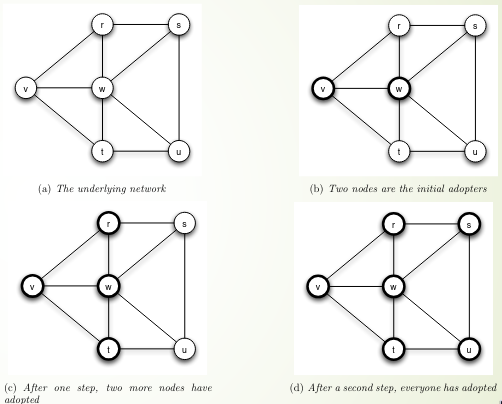
\includegraphics[width=0.5\linewidth]{images/Diff_ex1.png}
    \caption{Processo di diffusione in una rete}
    \label{fig:Diff_ex1}
\end{figure}

Se invece ponessimo come valori $a = 1$ e $b = 3$ , avremmo una soglia di adozione pari a $q = \frac{3}{4}$ , la quale non sarebbe sufficiente per la diffusione di $A$.

\subsection{Esempio 2}\label{sec:esempio2}

Consideriamo ora il processo di diffusione nella seguente rete (\autoref{fig:Diff_ex2}), e consideriamo due casistiche.

\begin{figure}[ht!]
    \centering
    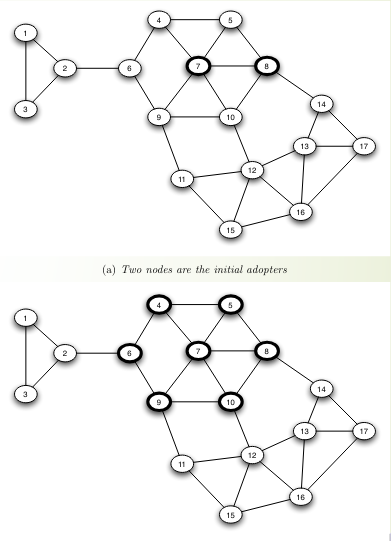
\includegraphics[width=0.25\linewidth]{images/Diff_ex2.png}
    \caption{Processo di diffusione in una rete}
    \label{fig:Diff_ex2}
\end{figure}

\begin{itemize}
    \item Se $a = 3$ e $b = 2$, allora $q = \frac{2}{5}$. In questo caso, (\autoref{fig:Diff_ex2}), lo stato $A$ è forzato sui nodi 7 e 8 e si diffonde solo sui nodi (4, 5, 6, 9, 10). Quindi $A$ non riesce a raggiungere i nodi fuori l'esagono.
    \item Se $a = 4$ e $b = 2$, allora $q = \frac{1}{3}$. In questo caso, dopo aver raggiunto tutti i nodi dell'esagono, $A$ è adottato anche da 2, 11 e 14, poi da 1, 3, 12, 13, 17 e infine da 15 e 16. In questo caso $A$, riesce a raggiungere tutti i nodi della rete.
\end{itemize}

Per riuscire ad ottenere una cascata completa, possiamo o aumentare il guadagno di $A$, oppure aumentare e/o cambiare i nodi iniziali nello stato $A$ (senza alterare la soglia d'adozione $q$ ). Per esempio consideriamo come insieme di nodi iniziali nello stato $A$ i nodi $\{2, 7, 8, 12\}$ (e ricordiamo che $q = \frac{2}{5}$ è rimasta invariata).

È facile osservare in questo caso che $A$ si propaga su tutta la rete.
Quindi, se non alteriamo $q$, viene da pensare che se il numero di nodi iniziali supera una certa soglia critica, allora avviene una cascata completa di $A$. In realtà l'avvenire di una cascata completa di $A$ non dipende solamente da quanti nodi iniziali sono forzati nello stato $A$, bensì anche dalla loro posizione. Per esempio se consideriamo altri 4 nodi iniziali $\{2, 7, 8, 14 \}$ non otterremo una cascata completa, nonostante ci siano lo stesso 4 nodi iniziali che adottano $A$.

\section{Cascate e Cluster}

\begin{definizione}[Insieme di Iniziatori]
    Definiamo l'insieme di nodi iniziatori $V_0$, l'insieme di nodi di partenza su cui viene forzato lo stato $A$. Indichiamo inoltre con $V_i$, l'insieme di nodi che adottano lo stato $A$ al passo $i$ del processo di diffusione.
\end{definizione}

\begin{definizione}[Cascata Completa]
    Definiamo il concetto di \textbf{cascata completa}, se ad un certo passo $t$, tutti i nodi hanno adottato $A$, ossia
    \[
    \text{se esiste } t \geq 0 \text{ tale che } \bigcup_{0 \leq i \leq t}V_i = V 
    \]

    Possiamo dire che la diffusione di $A$ si ferma quando 
    \[
    \bigcup_{i = 0}^{t} V_i = \bigcup_{i = 0}^{t+1} V_i
    \]
\end{definizione}

\begin{definizione}[Cluster di Densità $p$]
    Un \textbf{cluster di densità} $p$ è un sottoinsieme di nodi $V' \subseteq V$ tale che la frazione di vicini che ogni suo nodo ha in $V'$ è almeno $p$:
    \[
    \forall\ u \in V'\ \left[\frac{|N(u) \cap V'|}{|N(u)|} \geq p\right]
    \]
\end{definizione}

\begin{osservazione}
    Osservare anche che se $V',V''$ sono due cluster di densità $p$, allora anche $V' \cup V''$ è un cluster di densità $p$.
\end{osservazione}

\begin{proof}
Supponiamo $V'\cap V''=\varnothing$ e sia $u\in V'\cup V''$.

\textbf{Caso 1:} $u\in V'$. Allora, essendo $V'$ un cluster di densità $p$,
\[
\frac{|N(u)\cap V'|}{|N(u)|}\ge p.
\]
Poiché $V'\subseteq V'\cup V''$, si ha $N(u)\cap V'\subseteq N(u)\cap (V'\cup V'')$, dunque
\[
\frac{|N(u)\cap (V'\cup V'')|}{|N(u)|}\ge\frac{|N(u)\cap V'|}{|N(u)|}\ge p.
\]

\textbf{Caso 2:} $u\in V''$. Il ragionamento è identico scambiando i ruoli di $V'$ e $V''$.

Inoltre, poiché $V'\cap V''=\varnothing$, per ogni $u$ vale la relazione additiva
\[
|N(u)\cap (V'\cup V'')|=|N(u)\cap V'|+|N(u)\cap V''|,
\]
che mostra esplicitamente come i contributi provengano da insiemi disgiunti. Comunque, dai due casi precedenti segue che ogni nodo di $V'\cup V''$ ha almeno una frazione $p$ dei vicini nell'unione, quindi $V'\cup V''$ è un cluster di densità $p$.
\end{proof}

\begin{teorema}
    Sia $G = (V, E)$ un grafo e siano $V_0 \subseteq V$ l'insieme di nodi iniziatori e $q$ la soglia di adozione dello stato $A$.
    \[
        V_0 \text{ non genera una cascata completa}
        \quad\Longleftrightarrow\quad
        G \setminus V_0 \text{ contiene un cluster di densità } > 1-q .
    \]
\end{teorema}
\begin{proof}
    \mbox{}\\
    \textbf{($\implies$)}\; Supponiamo che $V_0$ non generi una cascata completa. In questo caso, esistono dei nodi che non adottano $A$. Quindi, sia $t$ il passo tale che $V_t \neq \emptyset$ e  $V_{t+1} = \emptyset$ (ossia $t + 1$ è il primo passo in cui $A$ non si diffonde più). Poniamo
    \[
    V_A = \bigcup_{0 \leq i \leq t} V_i
    \]
    l'insieme che contiene tutti e soli i nodi che adottano $A$. Poiché esistono nodi che non adottano $A$, allora $V \setminus V_A \neq \emptyset$. Poiché i nodi in $V \setminus V_A$ non adottano $A$, allora, \[
    \forall\ v \in V \setminus A\ \left[\frac{|N(v) \cap V_A|}{|N(v)|} < q\right]
    \]
    Quindi, poiché 
    \[
    \frac{|N(v) \cap V_A|}{|N(v)|} + \frac{|N(v) \cap (V \setminus V_A)|}{|N(v)|} = 1, \text{ allora } \frac{|N(v) \cap (V \setminus V_A)|}{|N(v)|} > 1-q
    \]
    In conclusione, $V \setminus V_A$ è un cluster di densità maggiore di $1 - q$ e $V \setminus V_A$ è contenuto in $G \setminus V_0$.
    \medskip

    \textbf{($\impliedby$)}\; Supponiamo ora che in $G \setminus V_0$ esista un cluster di densità maggiore di $1-q$. Ovvero, esiste $C \subseteq V \setminus V_0$ tale che, per ogni $v \in C$, $\frac{|N(v) \cap C|}{|N(v)|} > 1-q$.

    Supponiamo ora per assurdo che si generi una cascata completa: allora i nodi in $C$, prima o poi, adotteranno $A$. Sia $t$ il primo passo tale che $V_t \cap C \neq \emptyset$ (esistono nodi in $C$ che al passo $t$ hanno adottano $A$) ossia, per $i < t$, $V_i \cap C = \emptyset$ e di conseguenza esiste $u \in V_t \cap C$.

    Poniamo ora
    \[
    V' = \bigcup_{0 \leq i \leq t - 1} V_i
    \]
    l'insieme dei nodi che hanno adottato $A$ fino al passo $t - 1$, quindi $V'$ non contiene nessun nodo di $C$.
    Allora,
    \begin{itemize}
        \item Poiché $C$ è un cluster di densità $> 1 - q$ e $u \in C$, allora $\frac{|N(u) \cap C|}{|N(u)|} > 1-q$.
        \item Inoltre, poiché $u \in V_t$, allora $\frac{|N(u) \cap C|}{|N(u)|} \geq q$
    \end{itemize}
    Quindi, poiché $V' \cap C \neq \emptyset$, allora
    \[
    1  \textcolor{red}{ = } \frac{|N(u)|}{|N(u)|} \geq \frac{|N(u) \cap (C \cup V')|}{|N(u)|} = \frac{|N(u) \cap C|}{|N(u)|} + \frac{|N(u)| \cap V'|}{|N(u)|}  \textcolor{red}{ > } q + 1 - q = 1
    \]
    Trovando quindi un \textbf{\textcolor{red}{ASSURDO}}.
\end{proof}

Ciò che ci dice il precedente teorema è sostanzialmente che la presenza di cluster (con una certa densità) comporta un ostacolo alla diffusione di una innovazione $A$.

Ricordiamo dalle lezioni precedenti che generalmente i legami che collegano due comunità (o cluster) sono dei \textbf{legami deboli} (\textbf{weak ties}).
Infatti la forza dei \textbf{weak ties} è basata sull'idea che le connessioni sociali deboli (per esempio con persone che vediamo di rado) spesso formano \textbf{bridge edges} in una rete sociale.
Pertanto forniscono accesso a fonti di informazioni (per esempio nuove opportunità di lavoro) che risiedono in parti della rete a cui altrimenti non avremmo accesso.

Osserviamo inoltre che c'è una sostanziale differenza tra venire a conoscenza di una nuova idea e il decidere di adottarla.
Infatti considerando ancora l'esempio 2 (\autoref{sec:esempio2}), possiamo osservare che i nodi 4 e 9 vengono subito a conoscenza dell'innovazione $A$ in quanto entrambi sono vicini di un nodo iniziatore, però attendono più tempo prima di adottarlo.
Anche in un contesto sociale reale, sebbene una barzelletta o un video divertente online avanzano con una velocità notevole, la mobilitazione politica si muove più lentamente, avendo bisogno di prendere slancio all'interno di comunità.

La soglia di adozione $q$ offre una possibile spiegazione:
i movimenti sociali tendono ad essere imprese intrinsecamente rischiose, e quindi gli individui tendono a necessitare di soglie più elevate per la partecipazione.

Perciò possiamo concludere che mentre i \textit{weak-ties} che collegano due comunità differenti sono utilissimi alla diffusione di informazioni, allo stesso tempo sono un punto di debolezza (e quindi di ostacolo) per la diffusione di un'innovazione.

\newpage
\section{The Cascade Capacity on Infinite Network with bounded Degree}

In questa sezione analizzeremo in maniera più formale, tramite l'aiuto di alcuni esempi, se esiste e qual è la \textbf{threshold} (per una soglia di adozione) che scatena una cascata completa, anche con un insieme "piccolo" di nodi \textbf{iniziatori}.

Più in particolare analizzeremo il caso di reti con \textbf{infiniti nodi}, ma ognuno con \textbf{grado finito}. In questa maniera il concetto di \textit{insieme piccolo di iniziatori} è definito da qualsiasi \textbf{insieme finito}.


\begin{tcolorbox}[colback=white,colframe=black,title=Problema]
Dato un grafo regolare infinito \(G = (V, E)\), in cui ogni nodo possiede grado finito, si definisce la
\emph{soglia di adozione massima} \(q_{\mathrm{MAX}}\) come il valore più alto di \(q \in [0,1]\) per il quale
\emph{esiste} un insieme iniziale finito \(V_0 \subset V\) tale da innescare una cascata completa
nell'intero grafo secondo la dinamica di adozione basata sulla soglia.
\end{tcolorbox}

Il valore \(q_{\mathrm{MAX}}\) prende il nome di \textbf{capacità di cascata di} $G$.

\subsection{Esempio 1 - Catena Infinita}

Consideriamo una catena infinita di nodi, dove ogni nodo $i$ ha grado esattamente due ed incidente ai due archi $(i-1, i),\ (i, i+1)$.
Seppur tale insieme di nodi è equivalente all'insieme $\mathbb{Z}$, sappiamo che esiste una biezione con $\mathbb{N}$.

\begin{figure}[h!]
    \centering

    \begin{subfigure}{0.8\linewidth}
        \centering
        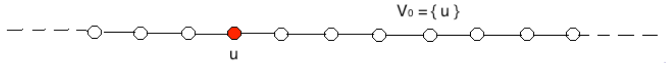
\includegraphics[width=\linewidth]{images/catena_infA.png}
        \caption{Primo caso: $V_0 = \{u\}$}
        \label{fig:catena_infinitaA}
    \end{subfigure}

    \vspace{0.5cm}

    \begin{subfigure}{0.8\linewidth}
        \centering
        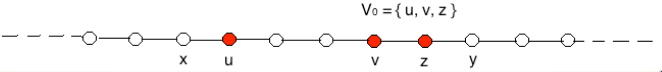
\includegraphics[width=\linewidth]{images/catena_infinitaB.png}
        \caption{Secondo caso: $V_0 = \{u, v, z\}$}
        \label{fig:catena_infinitaB}
    \end{subfigure}

    \caption{Grafo a catena infinita}
    \label{fig:catena_infinita}
\end{figure}


\begin{itemize}
    \item Se $|V_0| = 1$, ossia $V_0 = \{u\}$, allora occorre $q = \frac{1}{2}$ per generare una cascata completa, come mostrato in \autoref{fig:catena_infinitaA}.
    \item Se $|V_0| > 1$, ad esempio $V_0 = \{u, v, z\}$, è possibile generare una cascata con $q < \frac{1}{2}$? La risposta è \textbf{NO}, perché i nodi "al confine" con $V_0$, i nodi $x, y$ in \autoref{fig:catena_infinitaB}, hanno comunque bisogno di $q = \frac{1}{2}$ per passare ad $A$.
\end{itemize}

Quindi possiamo concludere che in una catena infinita, $q_{\mathrm{MAX}} = \frac{1}{2}$.

\newpage
\subsection{Esempio 2 - Grafo a Griglia Infinita}

Consideriamo ora una \textbf{griglia} infinita $\mathbb{Z} \times \mathbb{Z}$, dove ogni nodo è collegato coi nodi nelle rispettive posizione "UP", "DOWN", "LEFT", "RIGHT", "NE", "NW", "SE" e "SW".

\begin{figure}[ht!]
    \centering

    % Riga superiore
    \begin{subfigure}{0.23\linewidth}
        \centering
        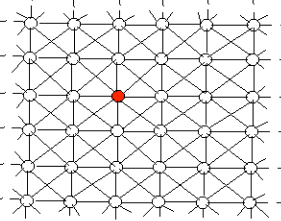
\includegraphics[width=\linewidth]{images/griglia.png}
        \caption{$|V_0| = 1$}
        \label{fig:griglia1}
    \end{subfigure}
    \hspace{0.1cm}
    \begin{subfigure}{0.23\linewidth}
        \centering
        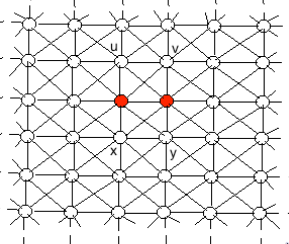
\includegraphics[width=\linewidth]{images/griglia2.png}
        \caption{$|V_0| = 2$}
        \label{fig:griglia2}
    \end{subfigure}

    % Riduzione drastica dello spazio verticale
    \vspace{0.2cm}

    % Riga inferiore
    \begin{subfigure}{0.23\linewidth}
        \centering
        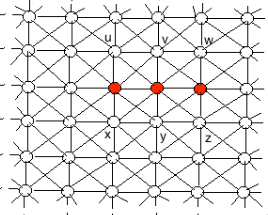
\includegraphics[width=\linewidth]{images/griglia3.png}
        \caption{$|V_0| = 3$}
        \label{fig:griglia3}
    \end{subfigure}
    \hspace{0.1cm}
    \begin{subfigure}{0.23\linewidth}
        \centering
        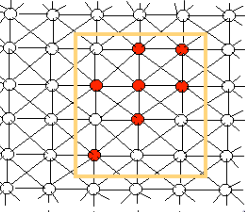
\includegraphics[width=\linewidth]{images/griglia4.png}
        \caption{$|V_0| > 3$}
        \label{fig:griglia4}
    \end{subfigure}

    \caption{Configurazioni di $V_0$ e soglie corrispondenti nella griglia.}
    \label{fig:griglia_totale}
\end{figure}


\begin{itemize}
    \item Se $|V_0| = 1$, allora occorre $q = \frac{1}{8}$ per generare una cascata completa.
    \item Se $|V_0| = 2$, allora $V_0$ contiene 2 nodi adiacenti e occorre $q = \frac{1}{4}$ per generare una cascata completa.
    \item Se $|V_0| = 3$, allora occorre $q = \frac{3}{8}$ per generare una cascata completa.
    \item Aumentando ulteriormente $|V_0|$, non si innalza più la soglia di adozione: per superare il rettangolo iniziale serve comunque $\frac{3}{8}$.
\end{itemize}

Allora, in una griglia infinita, $q_{\mathrm{MAX}} = \frac{3}{8}$.

\subsection{Soglia di Adozione Massima}

Dagli esempi precedenti è facile notare che la soglia di adozione massima nella griglia infinita è minore di quella della catena infinita, per via di una struttura più ricca è densa.
Comunque, in entrambi i casi, non si può mai avere una soglia di adozione maggiore di $\frac{1}{2}$

Quindi viene da pensare che, almeno in questi due modelli, l'innovazione $A$ deve essere appetibile almeno quanto lo stato dominante $B$.
In effetti questo è un ragionamento abbastanza ragionevole anche applicato in un contesto reale.

Sorge però la domanda:
\textit{Esiste una conformazione di una rete infinita in cui si può ottenere una capacita di cascata maggiore di $\frac{1}{2}$?}
\textit{Ovvero, è possibile fare in modo che si adotti $A$, nonostante $B$ sia più conveniente?}
Per fortuna la risposta è \textbf{NO}, e questo verrà dimostrato nel seguente teorema.

\begin{teorema}
    Per ogni grafo infinito $G=(V,E)$ i cui nodi hanno grado finito, la capacità di cascata di $G$ è al più $q_G \leq \frac{1}{2}$.
\end{teorema}

\begin{proof}
    Supponiamo per assurdo che esista un insieme finito di iniziatori $V_0$ che, con soglia di adozione $q > \frac{1}{2}$, generi una cascata completa.

    Indichiamo con $V_t$ l'insieme dei nodi che adottano $A$ al passo $t$. Sia, per ogni $t \geq 0$,
    \[
    S_t = \bigcup_{0 \leq i \leq t} Vi
    \]
    l'insieme dei nodi che, al passo $t$, sono nello stato $A$. 
    
    Definiamo l'\textbf{interfaccia $I_t$ al passo $t$} come l'insieme degli archi che, al passo $t$, hanno un estremo in $S_t$ e l'altro estremo in $V \setminus S_t$:
    \[
    I_t = \{(u, v) \in E: u \in S_t \land v \in V \setminus S_t\}
    \]
    In altre parole, $I_t$ è l'insieme di archi del \textbf{taglio} $(S_t, V \setminus S_t)$.

    Dato che $V_0$ genera una \textit{cascata completa} di $A$ con soglia di adozione $q > 0.5$, si può dimostrare che per ogni $t \geq 0$, allora è vero che 
    \[
    |I_t| > |I_{t+1}| \text{ oppure } I_t \equiv I_{t+1}
    \]

    Dato che il grado massimo di $G$ è \textbf{limitato}, allora $|I_0|$ sarà una quantità finita $k > 0$.
    Inoltre, è facile convincersi che il processo termina quando abbiamo che $I_t \equiv I_{t+1}$.
    
    Però visto che $V_0$ genera un processo \textbf{infinito} di cascata di $A$, allora per ogni $t \geq 0$, non deve mai accadere che $I_t \equiv I_{t+1}$, ovvero accade sempre che $|I_t| > |I_{t+1}|$.
    Ma ciò è assurdo, perché per via della dimensione finita di $I_0$, può accadere \textbf{al più} $k$ volte consecutive che il processo procedi.
    
    Perciò deve esistere necessariamente un tempo $\tau \geq k$, tale che $I_\tau \equiv I_{\tau + 1}$ (\textbf{\textcolor{red}{ASSURDO}}).

    Per farlo, basta dimostrare la \textbf{mutua esclusione} degli eventi, ovvero che se $I_t \not\equiv I_{t+1}$ allora necessariamente $|I_t| > |I_{t+1}|$\footnote{È stata applicata questa regola  $\lnot b \implies a \equiv a \lor b$ dove $a = |I_t| > |I_{t+1}|$ e $b = I_t \equiv I_{t+1}$.}.

    Quindi, se $I_t \not\equiv I_{t+1}$, allora esiste un nodo $v$ che adotta $A$ al passo $t + 1$, ossia $V_{t+1} \neq \emptyset$. Affinché ciò sia vero ($v \in V_{t+1}$), è necessario che $v$ abbia \textit{almeno} un vicino $u \in N(v)$ che è anche nello stato $A$, ovvero $u \in N(v) \cap S_t$. Più in generale, per ogni nodo $v \in V_{t+1}$ esiste almeno un arco del tipo $(u,v) \in I_t$, inoltre tale arco non apparterrà a $I_{t+1}$.
    Viceversa, tutti gli archi che apparterranno a $I_{t+1}$ certamente non erano in $I_t$.

    Quindi, per ogni $v \in V_{t+1}$,
    \begin{itemize}
        \item Gli archi incidenti su $v$ il cui altro estremo è in $S_t$ sono in $I_t$ ma non in $I_ {t+1}$ (come $(u,v)$ in \autoref{fig:PDdimostrazione}).
        \item Gli archi incidenti su $v$ il cui altro estremo è in $S_{t+1}$ sono in $I_{t+1}$ ma non in $I_t$ (come $(v, z)$ in \autoref{fig:PDdimostrazione}).
    \end{itemize}

    \begin{figure}[ht!]
        \centering
        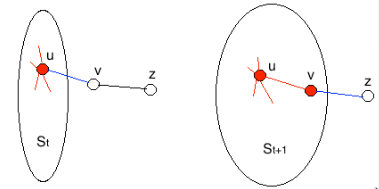
\includegraphics[width=0.5\linewidth]{images/PDdimostrazione.png}
        \caption{Gli archi di interfaccia sono disegnati blu}
        \label{fig:PDdimostrazione}
    \end{figure}

    Chiarito ciò, abbiamo che
    \[
    I_{t + 1} \equiv I_t \setminus \left[\bigcup_{v \in V_{t+1}} \lbrace (u,v) \in E : u \in S_t \right] \bigcup \left[\bigcup_{v \in V_{t+1}} \lbrace (z,v) \in E : z \in V \setminus S_{t+1} \right]
    \]

    È anche facile verificare che $\forall v,w \in V_{t+1},\ v \neq w$
    \begin{equation*}
        \begin{split}
        \{(u,v) \in E : u \in S_t \} &\cap \{ (u,w) \in E : u \in S_t \} = \emptyset\\
        &\land\\
        \{ (v,z) \in E : z \in V \setminus S_{t+1} \} &\cap \{ (w,z) \in E : z \in V \setminus S_{t+1} \} = \emptyset
        \end{split}
    \end{equation*}

    Per comprendere meglio ciò, visualizzare la \autoref{fig:PDdimostrazione2}

    \begin{figure}[ht!]
        \centering
        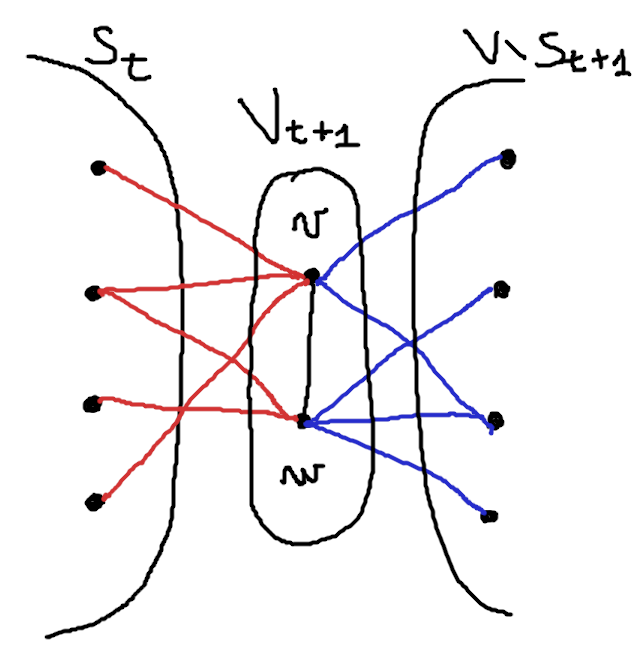
\includegraphics[width=0.3\linewidth]{images/PDdimostrazione2.png}
        \caption{Esempio}
        \label{fig:PDdimostrazione2}
    \end{figure}

    Tutto ciò implica che 
    \[
    |I_{t+1}| = |I_t| - \sum_{v \in V_{t+1}} |\{ (u,v) \in E : u \in S_t \}| + \sum_{v \in V_{t+1}} |\{ (v,z) \in E : z \in V \setminus S_{t+1} \}|
    \]

    Osserviamo ora, che,
    \[
    |\{ (u,v) \in E : u \in S_t \}| = |N(v) \cap S_t|
    \]
    e che
    \[
    |\{ (v,z) \in E : z \in V \setminus S_{t+1} \}| = |N(v) \setminus S_{t+1}|
    \]
    Infatti, per ogni \(v \in V_{t+1}\) vale che
    \[
    (u, v) \in I_t \iff u \in N(v) \cap S_t
    \]
    e analogamente
    \[
    (u,v) \in I_{t + 1} \iff u \in N(v) \setminus S_t
    \]
    Quindi, otteniamo
    \[
    |I_{t+1}| = |I_t| - \sum_{v \in V_{t+1}} |N(v) \cap S_t| + \sum_{v \in V_{t+1}} |N(v) \setminus S_{t+1}|
    \]

    Osserviamo adesso che, dato che un $v \in V_{t+1}$ ha adottato il nuovo stato $A$, e dato che la soglia di adozione è $q > \frac{1}{2}$, allora più della metà dei suoi vicini era in $S_t$, ovvero 
    \[
    \frac{| N(v) \cap S_t |}{| N(v) |} \geq q > \frac{1}{2}
    \]
    Oppure, visto in altri termini 
    \[
    | N(v) \cap S_t | > | N(v) \setminus S_t | \underbrace{>}_{\text{perché }S_t \subset S_{t+1}} | N(v) \setminus S_{t+1} |
    \]
    Allora, 
    \begin{align*}
        |I_{t+1}| &= |I_t| - \sum_{v \in V_{t+1}} |N(v) \cap S_t| + \sum_{v \in V_{t+1}} |N(v) \setminus S_{t+1}| \\
        &= |I_t| -  \sum_{v \in V_{t+1}} |N(v) \cap S_t| + |N(v) \setminus S_{t+1}| \\
        &\leq |I_t| - \sum_{v \in V_{t+1}} |N(v) \cap S_t| - |N(u) \setminus S_t|\\
        &= | I_t | - \sum_{v \in V_{t+1}} 1 = | I_t | - | V_{t+1} | \\ 
        &< | I_t |
    \end{align*}

dove l'ultima disuguaglianza viene dall'assunzione che $V_{t+1} \neq \emptyset$ e $S_t \subset S_{t+1}$.

Sia $q>\tfrac12$ e sia $V_0\subset V$ finito. Poiché ogni nodo ha grado finito, 
l'interfaccia iniziale ha dimensione finita, diciamo $|I_0|=k$. 
Dal fatto che per ogni $t\ge0$ si ha $|I_t|>|I_{t+1}|$ oppure $I_t=I_{t+1}$, 
segue che la situazione $I_t\neq I_{t+1}$ può verificarsi al più $k$ volte. 

Dunque esiste un tempo $\tau$ tale che per ogni $t\ge \tau$ vale $I_t=I_{t+1}$, 
e la diffusione si arresta. 
Tuttavia, in un grafo infinito una cascata completa richiede un processo che 
rimanga infinito nel tempo. Ne consegue che $V_0$ non può produrre 
una cascata completa.
\end{proof} 



\chapter{Herding}

Abbiamo visto che quando degli individui sono connessi tra di loro in una \textit{rete}, le loro decisioni e comportamenti possono essere influenzati (ed influenzare) da quello degli altri individui vicini.

Nello studio dei processi di diffusione abbiamo visto come il comportamento dei singoli individui veniva influenzato dalla diretta comunicazione col proprio vicinato. In questa sezione vedremo come le decisioni dei singoli individui possono essere influenzate dalle osservazioni fatte sul comportamento degli altri, senza lo scambio di alcuna informazione. In sostanza come è possibile estrapolare informazioni dal comportamento della massa.

Come primo esempio supponiamo di essere in vacanza in un nuovo posto e di dover scegliere un ristorante in cui mangiare. In base alle nostre ricerche personali scopriamo che il ristorante $A$ è il migliore che ci sia in zona, e quindi decidiamo di andarci. Poco prima di entrare vediamo che nel ristorante accanto, il ristorante $B$, c'è moltissima clientela, mentre il ristorante $A$ è praticamente vuoto. Non è del tutto irrazionale pensare che tutte le persone che vanno al ristorante $B$ abbiano \textbf{informazioni private} che noi non abbiamo, e supporre che in realtà il ristorante è il migliore. In effetti il fatto che il ristorante $A$ sia quasi vuoto non aiuta: verrebbe da pensare che siamo in possesso di informazioni non del tutto esatte o complete. Perciò decidiamo anche noi di andare al ristorante $B$.

In questo caso diremo che è avvenuta una \textbf{cascata informativa} (o \textbf{herding}). In poche parole, una cascata informativa occorre quando gli individui prendono decisioni in maniera sequenziale, osservando ciò che hanno fatto gli altri prima e cercando di inferire qualche informazione aggiuntiva che ha spinto gli altri ad agire in tale maniera

La cosa più interessante è che gli individui che “imitano” gli altri non lo fanno del tutto stupida, bensì facendo una serie di ragionamenti ed inferenze più che sensate. Naturalmente, l'imitazione può verificarsi anche a causa della pressione sociale all'esigienza di volersi conformare, senza alcuna causa informativa sottostante, e non è sempre facile distinguere questi due fenomeni. Consideriamo infatti l'esperimento di \textit{Milgram, Bickman e Berkowitz} del 1960, in cui venivano poste agli angoli delle strade dei gruppi di persone (da un minimo di 1 a un massimo di 15) a guardare il cielo senza alcun motivo. Si è osservato quanti passanti si sono fermati e hanno volto lo sguardo al cielo. Come prima osservazione si è visto che con una sola persona, pochissimi passanti si fermavano. Se invece 5 persone fissavano il cielo, alcuni passanti si fermavano a imitare, ma la maggior parte li ignorava. Infine, con un gruppo di 15 persone che guardano verso l'alto, hanno scoperto che il 45\% dei passanti imitava, fermandosi e guardare il cielo cercando di capire.

Quest'ultimo esperimento lascia pensare che esiste una \textbf{soglia critica} oltre la quale si scatena l'herding su una considerevole porzione di popolazione. Infatti, se camminando per strada vediamo due persone che fissano il cielo, è naturale pensare che i due individui non siano proprio sani mentalmente. Se invece ne vediamo 15, molto probabilmente guarderemo anche noi verso l'alto, per cercare di capire cosa c'è di interessante.

Alcune domande nascono spontanee:
\begin{itemize}
    \item esiste sempre una soglia critica che scatena l'herding di massa?
    \item e se esiste, come fare a trovarla?
\end{itemize}

\section{A Simple Herding Experiment: Il Gioco delle Urne}

Consideriamo un genere di gioco con la seguente tipologia di regole

\begin{enumerate}
    \item C'è una decisione da prendere
    \item I giocatori prendono le proprie decisioni in sequenza (uno dopo l'altro), e ogni persona può osservare le scelte fatte da coloro che hanno agito prima.
    \item Ogni giocatore ha alcune \textit{informazioni private} che aiutano a guidare la propria decisione.
    \item Un giocatore non può osservare direttamente le informazioni private che gli altri giocatori hanno, ma può trarre deduzioni su queste informazioni private da ciò che fanno.
\end{enumerate}

Secondo queste indicazioni, istanziamo un gioco con le seguenti regole:

\begin{itemize}
    \item C'è uno \textbf{scommettitore} in una stanza chiusa, e una serie di \textbf{giocatori} all'esterno.
    \item Lo scommettitore inserisce due palline rosse ed una blu in un'urna (che chiameremo $MR$, a Maggioranza Rossa), e due palline blu e una rossa in un'altra urna (che chiameremo $MB$, a Maggioranza Blu).
    \item Lo scommettitore poi mischia le due urne e ne sceglie una a caso (senza avere la possibilità di vederne il contenuto).
    \item Un giocatore alla volta entra nella stanza ed estrae una pallina dall'urna, e poi la reinserisce.
    \item Il giocatore comunica a tutti quanti se ritiene che l'urna sia $MR$ o $MB$ (sulla base delle sue informazioni). \textbf{Importante:} il giocatore non deve comunicare il colore della pallina pescata.
    \item Al termine vinceranno solo i giocatori che hanno indovinato quale urna è stata scelta inizialmente ($MR$ o $MB$).
\end{itemize}

Per definizione di questo gioco, l'informazione privata dei singoli giocatori è l'esito dell'estrazione (pallina blu o pallina rossa), e questa non viene mai condivisa con gli altri. Un giocatore però può inferire quale urna è meglio scegliere in base alle scelte fatte dagli altri prima (come vedremo adesso).

\begin{description}
    \item[Primo Giocatore:] Prima di estrarre la pallina, il primo giocatore è in possesso della sola informazione "l'urna è $MR$ o $MB$". Non avendo altre informazioni, a prescindere da cosa pescherà il primo giocatore, la probabilità che l'urna sia $MR$ o $MB$ è la stessa. Perciò gli conviene scomettere sul colore della pallina estratta: se pesca una pallina blu gli conviene scommettere su $MB$ (stesso discorso per $MR$).
    \item[Secondo Giocatore:] A questo punto il secondo giocatore può dedurre l'esito dell'estrazione del primo giocatore sulla base della sua scommessa. Senza perdita di generalità, supponiamo che il primo giocatore abbia scommesso $MB$ (e che quindi abbia estratto una pallina blu). Se il secondo estrae una pallina blu, allora sa che sono state estratte due palline blu consecutive, e che quindi è più conveniente scommettere su $MB$. Se invece estrae una pallina rossa, si ritrova nella stessa situazione inizale del primo giocatore (senza alcuna informazione rilevante), perciò gli conviene scommettere $MR$ in accordo alla sua estrazione.
    \item[Terzo Giocatore:] Anche il terzo giocatore è in grado di dedurre le estrazioni dei giocatori precedenti: se sono discordi allora sono avvenute due estrazioni discorde, se sono concorde allora sono avvenute due estrazioni di palline dello stesso colore. Consideriamo il caso in cui le prime due estrazioni siano discordi, in questo caso al terzo giocatore conviene rispondere in accordo a ciò che pesca (se pesca una pallina blu gli conviene votare $MB$, se ne pesca una rossa gli conviene votare $MR$). Consideriamo ora il caso in cui i primi due giocatori abbiamo voti condori, e senza perdita di generalità supponiamo che abbiano entrambi votato $MB$. Se il terzo giocatore pesca una pallina blu, allora vuol dire che sono state estratte tre palline blu di seguito, rafforzando la propbailità che $MB$ sia la risposta esatta. Se invece estrae una rossa, comunque è più probabile che la risposta esatta sia $MB$, perché sono state estratte due palline blu di seguito e poi una rossa. Quindi in ogni caso gli conviene votare $MB$.
    \item[Quarto Giocatore:] A questo punto il quarto giocatore può dedurre ciò che hanno fatto tutti i giocatori precedenti solamente se ci sono 2 voti concordi ed uno discorde (2 a 1). Perché se ci fossero 3 voti concordi, sappiamo che il terzo giocatore avrebbe votato in accordo ai primi due in ogni caso a prescindere dall'esito della sua estrazione. Supponiamo di essere nella situazione di "3 a 0" per $MB$. Al quarto giocatore conviene votare $MB$ in ogni caso (esattamente come per il terzo giocatore).     
\end{description}

A questo punto, dal quinto giocatore in poi, si genera una cascata informativa a favore di $MB$, a prescindere dalle singole estrazioni.

\section{Teorema di Bayes}

Al fine di formalizzare meglio la meccanica descritta sopra è necessario enunciare il \textbf{Teorema di Bayes}.

\begin{teorema}[di Bayes]
    Siano \(A\) e \(B\) due eventi con \(\Pr[B]>0\). Allora vale
    \[
    \Pr[A\mid B]=\frac{\Pr[B\mid A]\,\Pr[A]}{\Pr[B]}.
    \]
\end{teorema}

\begin{proof}
    Per definizione di probabilità condizionata abbiamo che
    \begin{align*}
        \Pr[A \mid B] = \frac{\Pr[A \cap B]}{\Pr[B]} \\
        \Pr[B \mid A] = \frac{\Pr[B \cap A]}{\Pr[A]}
    \end{align*}
    Da questo segue che:
    \[
        \Pr[A \cap B] = \Pr[A \mid B] \cdot \Pr[B] = \Pr[B \mid A] \cdot \Pr[A]
    \]
    Sostituendo opportunamente otteniamo l'enunciato del teorema
    \[
        \Pr[A \mid B] = \frac{\Pr[A \cap B]}{\Pr[B]} = \frac{\Pr[B \mid A]}{\Pr[B]} 
    \]
\end{proof}

\begin{definizione}[Probabilità Totale]
    Sia \(A\) un evento e sia \(\{B_i\}_{i=1}^n\) una partizione dello spazio campionario tale che \(\Pr[B_i]>0\) per ogni \(i\) e \(\bigcup_{i=1}^n B_i=\Omega\) con \(B_i\cap B_j=\varnothing\) per \(i\neq j\). Allora la probabilità di \(A\) si esprime tramite la formula della probabilità totale:
    \[
        \Pr[A]=\sum_{i=1}^n \Pr[A\mid B_i]\,\Pr[B_i].
    \]
    Più in generale, se \(\{B_i\}_{i\ge1}\) è una partizione numerabile, la somma è estesa su tutti gli indici.
    
    \begin{proof}
        Poiché \(A=\bigcup_{i=1}^n (A\cap B_i)\) è unione disgiunta, vale
        \[
            \Pr[A]=\sum_{i=1}^n \Pr[A\cap B_i]=\sum_{i=1}^n \Pr[A\mid B_i]\,\Pr[B_i],
        \]
        da cui l'enunciato.
    \end{proof}
\end{definizione}

Usando questa formula, possiamo riscrivere la formula di Bayes ne seguente modo:

\[
    \Pr[A\mid B]= \frac{\Pr[B\mid A]\,\Pr[A]}{\Pr[B]} = \frac{\Pr[B\mid A]\,\Pr[A]}{\Pr[B \mid A] \cdot \Pr[A] + \Pr[B \mid A^C] \cdot \Pr[A^C]}.
\]

Possiamo ora formalizzare l'esempio precedente utilizzando la formula di Bayes.

Definiamo gli eventi:
\begin{itemize}
    \item $MR$: l'urna è a maggioranza rossa;
    \item $MB$: l'urna è a maggioranza blu;
    \item $r$: la pallina estratta è rossa
    \item $b$: la pallina estratta è blu
\end{itemize}

Osserviamo inoltre che che i precedenti eventi sono mutualmente complementari.

\begin{align*}
    MR &= MB^C \\
    MB &= MR^C \\
    b &= r^C \\
    r &= b^C
\end{align*}

Secondo quindi le regole del gioco, sappiamo che

\begin{align*}
    \Pr[MR] &= \Pr[MB] = \frac{1}{2} \\
    \Pr[r \mid MR] &= \frac{2}{3}; \quad \Pr[b \mid MR] = \frac{1}{3}; \\
    \Pr[b \mid MB] &= \frac{2}{3}; \quad \Pr[r \mid MB] = \frac{1}{3}; 
\end{align*}

\begin{description}
    \item[Giocatore 1:] Supponiamo senza perdità di generalità che il giocatore 1 estrae una pallina blu, essi dovrà calcolare la probabilità che l'urna sia a maggioranza blu o rossa, e questo si può fare sfruttando il teorema di Bayes.
    \begin{align*}
        \Pr[MB \mid b] = \frac{\Pr[b\mid MB]\,\Pr[MB]}{\Pr[b \mid MB] \cdot \Pr[MB] + \Pr[b \mid MR] \cdot \Pr[MR]} = \frac{2}{3} \\[0.5cm]
        \Pr[MR \mid b] = \frac{\Pr[b\mid MR]\,\Pr[MR]}{\Pr[b \mid MR] \cdot \Pr[MR] + \Pr[b \mid MB] \cdot \Pr[MB]} = \frac{1}{3}
    \end{align*}
    \item[Giocatore 2:] Vediamo ora quale strategia è migliore per il secondo giocatore. Consideriamo come prima situazione quella in cui esso estrae una pallina rossa, ed indichiamo con \textbf{br} l'evento \textit{sono state estratte in ordine una pallina blu e poi una rossa}. Dato che il secondo giocatore sa esattamente cosa ha pescato il primo (dato che lo può inferire con certezza assumendo che il primo giocatore giochi correttamente), si può affermare che il secondo giocatore si trova a dover calcolare le seguenti probabilità:
    \begin{align*}
        \Pr[MB \mid br] = \frac{\Pr[br\mid MB]\,\Pr[MB]}{\Pr[br \mid MB] \cdot \Pr[MB] + \Pr[br \mid MR] \cdot \Pr[MR]} = \frac{1}{2} \\[0.5cm]
        \Pr[MR \mid br] = \frac{\Pr[br\mid MR]\,\Pr[MR]}{\Pr[br \mid MR] \cdot \Pr[MR] + \Pr[br \mid MB] \cdot \Pr[MB]} = \frac{1}{2}
    \end{align*} 
    Perciò il secondo giocatore non può estrarre alcuna informazione utile dall'estrazione del primo, e quindi gli conviene scommettere in accordo a ciò che estrae.

    Consideriamo ora il caso in cui il secondo giocate estrae una pallina blu. In questo l'informazione riguardo la prima estrazione è realmente utile, in quanto possiamo dire che la probabilità è nettamente più sbilanciata verso $MB$
    \begin{align*}
        \Pr[MB \mid bb] = \frac{\Pr[bb\mid MB]\,\Pr[MB]}{\Pr[bb \mid MB] \cdot \Pr[MB] + \Pr[bb \mid MR] \cdot \Pr[MR]} = \frac{4}{5} \\[0.5cm]
        \Pr[MR \mid bb] = \frac{\Pr[bb\mid MR]\,\Pr[MR]}{\Pr[bb \mid MR] \cdot \Pr[MR] + \Pr[bb \mid MB] \cdot \Pr[MB]} = \frac{1}{5}
    \end{align*}
    \item[Giocatore 3:] A questo punto (sempre supponendo che la prima estrazione sia stata una pallina blu) possiamo essere in due situazioni differenti
    \begin{itemize}
        \item $br$: sono avvenute in sequenza le estrazioni blu-rossa
        \item $bb$: sono avvenute in sequenza le estrazioni blu-blu
    \end{itemize}
    Per semplicità consideriamo solo il caso $bb$.
    
    Se il terzo giocatore estrare una pallina blu, allora le probabilità che deve calcolare sono:
    \begin{align*}
        \Pr[MB \mid bbb] = \frac{\Pr[bbb\mid MB]\,\Pr[MB]}{\Pr[bbb \mid MB] \cdot \Pr[MB] + \Pr[bbb \mid MR] \cdot \Pr[MR]} = \frac{8}{9} \\[0.5cm]
        \Pr[MR \mid bbb] = \frac{\Pr[bbb\mid MR]\,\Pr[MR]}{\Pr[bbb \mid MR] \cdot \Pr[MR] + \Pr[bbb \mid MB] \cdot \Pr[MB]} = \frac{1}{9}
    \end{align*}
    Se invece il terzo giocatore estrare una pallina rossa, allora le probabilità che deve calcolare sono:
    \begin{align*}
        \Pr[MB \mid bbr] = \frac{\Pr[bbr\mid MB]\,\Pr[MB]}{\Pr[bbr \mid MB] \cdot \Pr[MB] + \Pr[bbr \mid MR] \cdot \Pr[MR]} = \frac{1}{3} \\[0.5cm]
        \Pr[MR \mid bbr] = \frac{\Pr[bbr\mid MR]\,\Pr[MR]}{\Pr[bbr \mid MR] \cdot \Pr[MR] + \Pr[bbr \mid MB] \cdot \Pr[MB]} = \frac{2}{3}
    \end{align*}
    In questo caso al giocatore 3 conviene votare in accordo a ciò che hanno votato i primi due giocatori, a prescindere da quale sarà l'esito della sua estrazione.
    \item[Giocatore 4:] 
\end{description}
\include{SistemiDiVoto}
\chapter{WebSearch}

\section{World Wide Web}

Il Web è un'applicazione sviluppata da \textbf{Tim Berners-Lee}, nel periodo 1989-1991 per consentire alle persone di condividere infomrazioni tramite Internet.

L'architettura del web è di tipo \textbf{client-server} e il suo funzionamento può essere descritto come segue:

\begin{itemize}
    \item Le informazioni sono salvate su delle macchine \textbf{server} e resi disponibili tramite Internet sotto forma di \textbf{pagine web}.
    \item Un'applicazione \textbf{client} (browser) richiede tali pagine web pubblicamente accessibili.
\end{itemize}

A noi ciò che interessa in realtà non è \textbf{l'organizzazione fisica} ma quella \textbf{logica} delle pagine web.Le pagine web possono \textbf{referenziare} in maniera \textit{diretta} altre pagine web, tramite dei \textbf{riferimenti} o \textbf{link}. Possiamo quindi pensare al web come un grafo diretto in cui i nodi sono le pagine web, e gli archi sono i riferimenti tra una pagina e un'altra. Per questo motivo, una pagina web viene anche detta \textbf{ipertesto}.

\subsection{Precursori dell'Ipertesto}

Possiamo considerare l'ipertesto come un'implementazione del concetto di \textbf{memoria associativa}. Un primo precursore all'ipertesto è il concetto di \textbf{referecence}, ad esempio,  le citazioni all'interno di articoli o libri ad altre informazioni o autori di tali infomrazioni. Anche in questo caso si crea un grafo diretto i cui nodi sono i libri o gli articoli e gli archi sono  riferimenti.La differenza sostanziale però con l'ipertesto è la linea temporale nella quale si fanno i riferimenti. Se un libro $X$ fa una citazione a un articolo $Y$ vuol dire che $Y$ è stato scritto e pubblicato prima di $X$, perciò non ci potranno essere riferimenti ad $X$ nell'articolo $Y$.

Invece, nel grado del web capita spesso di avere archi bidirezionali, ovvero due pagine che si referenziano a vicenda.

Un altro precursore dell'ipertesto sono le cosidette \textbf{crossing-referecences}, o \textbf{riferimenti incrociati}. Tale tipo di organizzazione la troviamo per esempio in un enciclopedia, e consente di collegare argomenti differenti attraverso una catena di collegamenti semantici o riferimenti tra altri argomenti.

\begin{figure}[ht!]
    \centering
    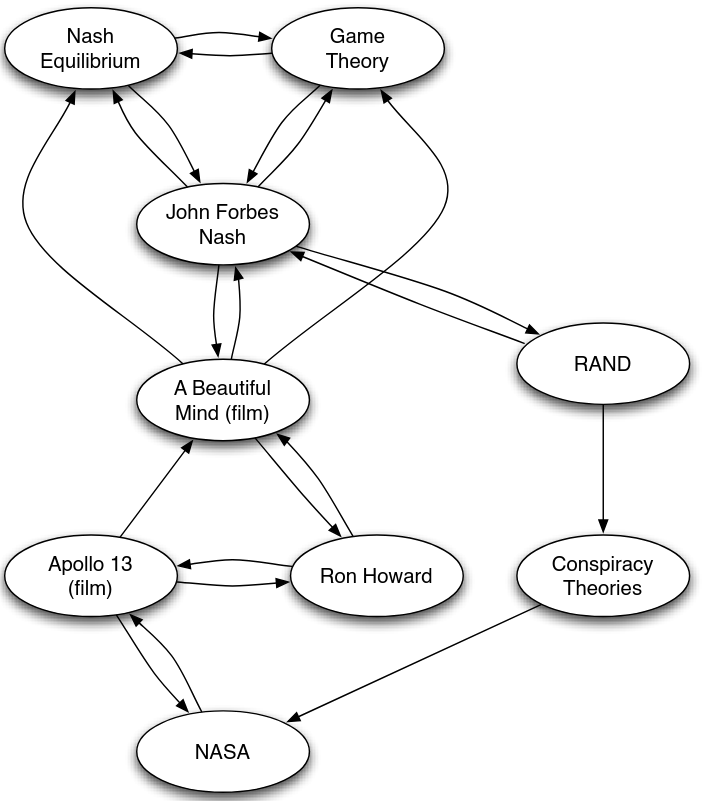
\includegraphics[width=0.5\linewidth]{images/WS_references.png}
    \caption{Esempio di crossing-referecences}
    \label{fig:WS_references}
\end{figure}

\subsection{MEMEX}

Vannevar Bush nel suo articolo "As we may think" del 1945 cercò di immaginare come le moderne tecnologie di comunizaione emergenti all'epoca avrebbero influenzato il mondo, grazie alle rivoluzionarie tecniche di \textbf{archiviazione, scambio} e \textbf{accesso} di informazioni.

In particolare Bush osservò che i metodi tradizionali per archiviare le informazioni in un libro, in una biblioteca o nella memoria di un computer erano altamente \textbf{lineari}. Basta pensare a un dizionario enciclopedico in cui tutti gli argomenti sono ordinati uno dopo l'altro.

D'altra parte la mente umana struttura e accede alla propria esperienza mostrando quella che potrebbe essere definita una \text{memoria associativa}, ovvero è strutturata in una \textbf{rete semantica} di concetti. Tu pensi a una cosa, te ne ricorda un'altra tramite una \textit{connessione}, dopodiché ti viene un intuizione che ti porta ad un terzo pensiero, e così via…

Bush ha quindi immaginato un sistema che cercava di imitare questo stile di memorizzazione \textbf{associativa}, il \textbf{MEMEX}, ovvero una versioni digitalizzate di tutta la conoscenza umana collegate da collegamenti associativi. Infatti Bush fu esplicitamente citato da Tim Berners Lee quando progettò il Web.

\subsection{Web 2.0}

Inizialmente, il web era costituito da una collezione di pagine \textbf{statiche} al cui interno erano (eventualmente) presenti degli \textit{hyperlink} ad altre pagine. Tali \textit{hyperlink} sono detti \textbf{navigazionali} in quanto servono appunto a "navigare" nel Web, esattamente come noi navighiamo nella nostra conoscenza, implmentando quindi il conetto di \textbf{memoria associativa}.

Col tempo però il web si è evoluto, passando da pagine totalmente statiche a pagine che consentono di effettuare \textbf{azioni}, come per esempio effettuare una richiesta ad un server oppure effettuare pagamenti. I link che consentono di effettuare tali azioni prendono il nome di link \textbf{transazionali}.

Altre evoluzioni sono per esempio l'avvento dei servizi, come per esempio:
\begin{itemize}
    \item La creazione e mantenimento di contenuti in maniera condivisa con Wikipedia.
    \item Lo scambio di messaggio con i servizi di web-mailing.
    \item Reti che connettono individui anziché documenti con i social-media.
    \item Reti che connettono video con YouTube.
\end{itemize}

Con tali evoluzioni si indica il cosidetto Web 2.0.

\subsection{Il Grafo Diretto del Web}

Il Web può essere visto come un grafo diretto, i cui nodi sono le \textbf{pagine} e gli archi sono gli \textbf{hyperlink} tra esse. Inoltre, è facilmente osservabile che una pagina web conosce solamente le pagine a cui stan puntando (\textbf{archi uscenti}) e non le pagine che la stanno puntando (\textbf{archi entranti}).

In uno studio del 2000, si è osservato che il grafo del web è è composto da milioni di nodi, ed ha una forma a \textbf{bowtie (a fiocco)}. Come si può osservare in \autoref{fig:WS_bowtie}, al centro è presente una \textbf{componente gigante fortemente  connessa} composta appunto dalla maggior parte dei nodi. In tale componente, per ogni pagina $X$ della componente è possibile trovare una serie link che collegano $X$ verso qualsiasi nodo della SCC, e viceversa da qualsiasi altra pagina è possibile navigare e raggiungere $X$.

\begin{figure}[ht!]
    \centering
    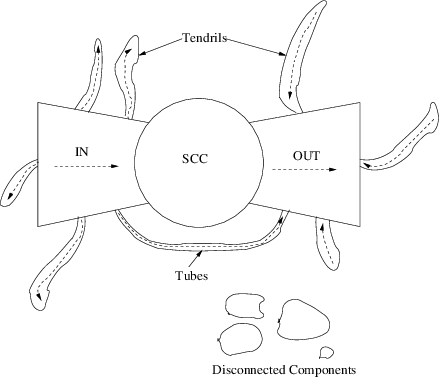
\includegraphics[width=0.5\linewidth]{images/WS_bowtie.png}
    \caption{Il grafo del web come \textbf{bowtie}}
    \label{fig:WS_bowtie}
\end{figure}

Dopodiché, si osservo la presenza di altre 2 componenti che formavano una sorta di \textit{flusso} in entrata e in uscita da SCC, le quali sono:

\begin{itemize}
    \item \textbf{IN}: composta dai nodi dai quali navigando è possibile raggiungere SCC, ma non raggiungibili in alcun modo da SCC.
    \item \textbf{OUT}: composta dai nodi raggiungibili da SCC tramite una navigazione ma che a loro volta non possono raggiungere SCC. Possiamo quindi die che questa componente rappresenta il flusso in uscita da SCC.
\end{itemize}

Infine, sono state individuate altre componenti nel grafo del web:

\begin{itemize}
    \item \textbf{Tendrilis}: detti anche \textit{tentacoli}, è una componente composta da 
    nodi che sono raggiungibili dai nodi presenti nella componente IN ma dai quali non si può raggiungere SCC e da nodi attraverso i quali si può raggiungere la componente OUT ma i quali non sono raggiungibili dai nodi in SCC.
    \item \textbf{Tubi}: composto dai nodi che creano un flusso che collega la componente IN alla componente OUT senza passare però per la componente SCC.
    \item \textbf{Componenti disconnesse}: una serie di nodi disconnessi dalla struttura a fiocco.
\end{itemize}

\section{Web Search}

Il problema di classificare e ricercare documenti è un problema antico.

Prima dell'avvento del Web, la difficoltà nel ricercare documenti era sostanzialmente dovuta alla scarsità di questi ultimi. Infatti, un tempo bisognava raggiungere fisicamente una biblioteca, libreria o archivio per avere accesso a libri, articoli o documenti, e inoltre non ce n'erano a disposizione una grande quantità. Tuttavia c'era un vantaggio, i documenti in generale erano catalogati in categorie, perciò a chi interessava avere informazioni su un determinato argomento bastava recarsi nel luogo in cui erano raccolti i documenti relativi all'argomento interessato. Per esempio, a un avvocato che necessita delle schede penali di alcune persone basta andare in un archivio di un tribunale. Oppure se ti interessa trovare un nuovo romanzo da leggere, basta andare in libreria nella sezione "Romanzi" e troverai una raccolta di libri inerenti al genere che ti interessa.

Il Web ha letteralmente capovolto i ruoli. Adesso chiunque ha acesso a una infinità di documenti in letteralmente pochissimi istanti. Il problema principale invece è appunto questa \textbf{sovrabbondanza di documenti}, i quali purtroppo non sono catalogati e raggruppati in categorie.

Purtroppo proprio per questa eterogeneità dei documenti, non è possibile effettuare una ricerca specializzata per parole chiave. Oltre al fatto che il numero di parole chiave è potenzialmente illimitato, una parola assume differenti significati. Infatti per esempio la parola "albero" in teoria dei grafi è un grafo particolare, mentre in botanica è un tipo di pianta, oppure ancora può poter significare un albero genealogico.

Si vuole quindi definire uno strumento di web search che consenta di effettuare una ricerca catalogando in base a delle parole chiave e scartando tutte le pagine non coerenti. Questa però non è una condizione sufficiente affinché uno strumento di web search risulti utile. Infatti, come risultato di una ricerca, potrebbe essere restituito un insieme potenzialmente immenso di pagine inerenti alle parole chiave. Perciò è necessario che tale strumento in qualche modo sfoltisca le pagine meno rilevanti, restituendo così un inseme abbastanza piccolo da essere umanamente visitato, e possibilmente ordinando queste pagine in un ordine di rilevanza, ovvero effettuando un \textbf{ranking} delle pagine restituite.

\subsection{Link Analisys}

Purtroppo il contenuto interno di una pagina non consente da solo di quantificarne con precisione la sua rilevanza rispetto alla ricerca in corso.

Un primo strumento utile che consente invece di capire meglio la rilevanza di una pagina sono gli \textbf{hyperlink}. 

Consideriamo prima un esempio:

Stiamo studiando un articolo utile per fare una tesi. Per capire meglio l'argomento un solo articolo non basta, perciò decidiamo di attingere alla bibliografia dell'articolo. Purtroppo notiamo che sono presenti svariate decine di citazioni ad altri articoli. Non potendo leggerli tutti quanti, è sensato considerare gli articoli che più hanno citazioni in generale.

Prendendo quindi come base questo esempio, dopo aver escluso tutte quelle pagine non inerenti alla nostra ricerca, possiamo \textbf{ordinarle} in ordine non crescente di numero di referimenti. Più precisamente, mettiamo tra i primi risultati della ricerca tutte quelle pagine che all'interno del sottoinsieme di pagine inerenti alla ricerca sono \textbf{maggiormente puntate da hyperlink}.

Ovvero la rilevanza di una pagina è calcolata analizzando i link che la coinvolgono.

\subsection{Metodo HITS}

Il primo metodo di link analisys che studiamo è il  metodo \textbf{HITS - Hyperlink-Induced Topic Search}.

Poiché consideriamo come pagine rilevanti le pagine che sono molto puntate da altre pagine nell'insieme, può accadere che una pagina è puntata da tante pagine poco rilevanti ai fini della ricerca, ad esempio, sappiamo che per finalità di marketing possono essere acquistati puntatori
ad una data pagina, così da far aumentare il suo contatore di \textbf{in-link}. Allora è necessario considerare la seguente questione:

\textit{Quando una pagina è considerata abbastanza autorevole da trasmettere rilevanza ad una pagina a cui punta?}

Il metodo HITS, associa a ciascuna pagina 2 indici:

\begin{itemize}
    \item Un indice di \textbf{autorità}: questo indice esprime la \textit{rilevanza} della pagina ai fini della ricerca.
    \item Un indice di \textbf{hub (centro, fulcro)}: questo indice esprime \textit{l'autorevolezza} della pagina a conferire autorità alle pagine alle quali punta. In altre parole indica quanto questa pagine è rilevante per la pagine a cui punta.
\end{itemize}

Intuitivamente, possiamo definire l'indice d'autorità $a_i$ della pagina $i$, come il numero di pagine attinenti alla ricerca che puntano alla pagina $i$ (\textbf{In-Degree})
\[
    a_i = |\{j: j \text{ è attinente alla ricerca e } j \rightarrow i\}|
\]

In questo modo, se consideriamo la matrice $M$ di adiancenza del sottografo del Web attinente alla ricerca, abbiamo che
\[
a_i = \sum_{j=1}^n M_{ji}
\]

Analogamente, il valore di hub $h_i$ di una pagina $i$, potrebbe essere il numero di pagine attinenti alla ricerca alle quali essa punta (\textbf{Out-Degree})

\[
    h_i = |\{j: j \text{ è attinente alla ricerca e } i \rightarrow j\}|
\]

di conseguenza, abbiamo che

\[
h_i = \sum_{j=1}^n M_{ij}
\]

dove la matrice di adiacenza $M$ del sottografo rilevante è definita come
\[
M_{ij} =
\begin{cases}
1 & \text{se } i \rightarrow j,\\[4pt]
0 & \text{altrimenti,}
\end{cases}
\qquad\text{per } i,j = 1,\dots,n.
\]


Raffiniamo il modello introducendo una dipendenza ricorsiva tra i punteggi: il punteggio di \textbf{Autorità ($a_i$)} di una pagina è proporzionale alla somma dei punteggi di \textbf{Hub} delle pagine che la puntano. Simmetricamente, il punteggio di \textbf{Hub ($h_i$)} è proporzionale alla somma dei punteggi di \textbf{Autorità} delle pagine verso cui essa punta.

\begin{itemize}
    \item Una pagina è una buona \textbf{Authority} se è linkata da ottimi \textbf{Hub}.
    \item Una pagina è un buon \textbf{Hub} se linka ottime \textbf{Authority}.
\end{itemize}

Quindi, se supponiamo di conoscere un valore iniziale di Hub, $h_i^{(0)}$ per ciascuna pagina $i$, allora

\[
a_i^{(1)} = \sum_{j=1}^n M_{ji} h_j^{(0)}
\]

e poiché il valore di autorità di ciascuna pagina è variato, potremmo calcolare il valore di hub per ottenere una valutazione migliore, ossia

\[
h_i^{(1)} = \sum_{j=1}^n M_{ij} a_j^{(1)}
\]

Quindi, al passo $k$, abbiamo che

\begin{equation}\label{eq:auth_and_hub}
\begin{split}
    a_i^{(k+1)} &= \sum_{j=1}^n M_{ji} h_j^{(k)} \\
    h_i^{(k+1)} &= \sum_{j=1}^n M_{ij} a_j^{(k+1)}
\end{split}
\end{equation}

definendo quindi un metodo iterativo per il calcolo dei valori di autorità e hub.

Poiché in genere non si hanno informazioni iniziali circa il valore del hub delle pagine che si stanno considerando, si può assumere che tali valori siano uguali per tutte le pagine, ossia
\[
\forall i = 1, \dots n,\ h_i^{(0)} = 1.
\]
Inoltre, possiamo riscrivere le equazioni \eqref{eq:auth_and_hub} nel seguente modo:

\begin{equation}
\begin{split}
    a^{(k+1)} &= M^T\ h^{(k)} \\
    h^{(k)} &= M\ a^{(k)}
\end{split}
\end{equation}

dove $a^{(k+1)}$ e $h^{(k)}$ sono vettori colonna.

Abbiamo quindi introdotto un procedimento iterativo che aggiorna progressivamente i punteggi di hub e di authority per ciascuna pagina. L'obiettivo è che, ad ogni passo, tali valori riflettano sempre meglio la rilevanza delle pagine; perché questo avvenga è però necessario che la procedura converga verso dei valori limite, che costituiscono i punteggi "reali" di hub e authority.

Le relazioni che aggiornano i vettori $a^{(k)}$ e $h^{(k)}$ sono somme di termini non negativi; di conseguenza i loro valori tendono ad aumentare con le iterazioni e non convergono verso un vettore limite. Perciò la convergenza ha senso solo dopo l'applicazione di un'opportuna \textbf{normalizzazione}.

\begin{teorema}\label{teo:th_hits}
    Esistono un valore \(c\in\mathbb{R}_{>0}\) e un vettore \(z\in\mathbb{R}^n\), \(z\neq 0\), tali che per ogni vettore iniziale \(h^{(0)}\) con coordinate strettamente positive si ha
    \[
        \lim_{k\to\infty}\frac{h^{(k)}}{c^k}=z
        \qquad\text{e}\qquad
        \lim_{k\to\infty}\frac{a^{(k)}}{c^k}=z.
    \]
\end{teorema}

\newpage

\subsubsection{Richiami di Algebra Lineare}

Prima di dimostrare questo teorema è necessario ricordare alcune nozioni di algebra lineare.

\begin{definizione}[Autovalore e Autovettore]
    Data una matrice quadrata $A \in \mathbb{R}^{n\times n}$, un vettore $x \in \mathbb{C}^n$ e un valore $\lambda \in \mathbb{C},\ \lambda \neq 0$, diremo che $x$ e $\lambda$ sono rispettivamente un \textbf{autovettore} e un \textbf{autovalore} per $A$ se e solo se
    \[
        Ax = \lambda x
    \]
\end{definizione}

\begin{teorema}\label{teo:th_rosso}
    Sia \(A\in\mathbb{R}^{n\times n}\) simmetrica. Allora tutti gli autovalori di \(A\) sono reali (contati con la molteplicità) ed esiste una base ortonormale di \(\mathbb{R}^n\) formata da autovettori di \(A\).
\end{teorema}

\begin{definizione}[Base]
    Un insieme di vettori $\{z_1,\dots,z_n\}\subset\mathbb{R}^n$ si dice \textbf{base} di $\mathbb{R}^n$ se soddisfa una (e quindi entrambe) delle seguenti proprietà equivalenti:
    \begin{enumerate}
        \item ogni vettore $x\in\mathbb{R}^n$ si può esprimere come combinazione lineare dei $z_i$, ovvero esistono scalari $c_1,\dots,c_n\in\mathbb{R}$ tali che
        \[
            x=\sum_{i=1}^n c_i z_i;
        \]
        \item i vettori $z_1,\dots,z_n$ sono linearmente indipendenti.
    \end{enumerate}
    Inoltre, in questo caso la scrittura di $x$ come combinazione lineare dei $z_i$ è unica.
\end{definizione}

\begin{definizione}[Ortonormale]
    Sia $\{z_1,\dots,z_n\} \subset \mathbb{R}^n$, con $z_i=(z_{i1},\dots,z_{in})$.
    Diciamo che la famiglia è \emph{ortonormale} se per ogni \(i=1,\dots,n\) vale \(\|z_i\|=1\) e per ogni \(i\neq j\) si ha \(\langle z_i,z_j\rangle=0\).
\end{definizione}

\begin{definizione}[Matrice semidefinita positiva]
    Una matrice simmetrica \(A\in\mathbb{R}^{n\times n}\) si dice \emph{semidefinita positiva} se
    \[
        \forall x\in\mathbb{R}^n:\quad x^{T} A x \ge 0.
    \]
\end{definizione}

\begin{teorema}\label{teo:th_blu}
    Sia $A\in\mathbb{R}^{n\times n}$ una matrice semidefinita positiva. Allora:
    \begin{enumerate}
        \item tutti gli autovalori di $A$ sono maggiori o uguali a $0$;
        \item se $A\neq 0$, allora esiste almeno un autovalore strettamente positivo.
    \end{enumerate}
\end{teorema}

\newpage

\subsubsection{Dimostrazione del Teorema}

Dimostriamo ora il \autoref{teo:th_hits} usando i due teoremi appena enunciati, \autoref{teo:th_rosso} e \autoref{teo:th_blu}.

\begin{proof}[\autoref{teo:th_hits}]
    Per iniziare la dimostrazione, richiamiamo le espressioni per gli indici di autorità e hub:
    \[
    \begin{aligned}
        a^{(k+1)} &= M^T h^{(k)},\\
        h^{(k)}   &= M a^{(k)}.
    \end{aligned}
    \]

    \begin{description}
        \item[Osservazione 1.] La matrice $M M^T$ è reale e simmetrica:
        \[
        (M M^T)_{ij}=\sum_{k=1}^{n}M_{ik}(M^T)_{kj}=\sum_{k=1}^{n}M_{ik}M_{jk}=(M M^T)_{ji}.
        \]
        Per il \autoref{teo:th_rosso}, $M M^T$ ammette una base ortonormale di autovettori e tutti i suoi autovalori sono reali.
        \item[Osservazione 2.] $M M^T$ è semidefinita positiva: per ogni $x\in\mathbb{R}^n$
        \[
        x^T(M M^T)x=(x^T M)(M^T x)=\|M^T x\|^2\ge 0.
        \]
        infatti, ponendo
        \begin{align*}
            &y = (M^T x) = (y_1, y_2, \dots, y_n) \\
            &y^T = (x^T M) = (y_1, y_2, \dots, y_n)^T
        \end{align*}
        si ottiene
        \[
        x^T(M M^T)x = (x^T M)(M^T x) = y^T\ y = \sum_{k=1}^{n} y^2_{k} \ge 0
        \]
        Essendo $M M^T\neq 0$, dal \autoref{teo:th_blu} segue che il suo autovalore massimo è strettamente positivo.
    \end{description}

    Usando le relazioni ricorsive otteniamo:
    \[
    \begin{aligned}
        h^{(1)} &= M a^{(1)} = M M^T h^{(0)},\\
        h^{(2)} &= M a^{(2)} = (M M^T) h^{(1)} = (M M^T)^2 h^{(0)},\\
        &\ \vdots\\
        h^{(k)} &= (M M^T)^k h^{(0)}.
    \end{aligned}
    \]

    Sia ora $\{z_1,\dots,z_n\}$ una \textbf{base ortonormale} di autovettori reali di $MM^T$, con autovalori non negativi corrispondenti $c_1,\dots,c_n$ tali che
    \[
    (MM^T) z_i = c_i z_i,\qquad i=1,\dots,n.
    \]
    Senza perdita di generalità ordiniamo gli autovalori in modo decrescente:
    \[
    c_1 \ge c_2 \ge \dots \ge c_n,
    \]
    ricordando che $c_1>0$.
    Possiamo quindi esprimere $h^{(0)}$ come combinazione lineare degli autovettori:
    \[
    h^{(0)} = \sum_{i=1}^{n} q_iz_i \text{ scelti opportuni scalari } q_i 
    \]

    Di conseguenza, 
    \begin{align*}
        h^{(k)} &= (M M^T)^k h^{(0)} = (M M^T)^k \sum_{i=1}^{n} q_iz_i \\
        &= (M M^T)^{k-1} \sum_{i=1}^{n} q_i (M M^T) z_i = (M M^T)^{k-1} \sum_{i=1}^{n} q_i c_i z_i \text{ per definizione di autovalore} \\
        &= (M M^T)^{k-2} \sum_{i=1}^{n} q_i c_i (M M^T) z_i = (M M^T)^{k-2} \sum_{i=1}^{n} q_i c_i^2 z_i \\
        &\vdots \\
        h^{(k)} &= \sum_{i=1}^{n} q_i c_i^k z_i
    \end{align*}

    Dividiamo ora entrambi i membri per $c_1^k$ e otteniamo
    \[
    \frac{h^{(k)}}{c_1^k} = \sum_{i=1}^{n} q_i \left(\frac{c_i}{c_1} \right)^k z_i
    \]

    Poiché l'autovalore massimo può presentarsi con molteplicità maggiore di uno, indichiamo con \(l\) (con \(1\le l\le n\)) il numero di autovalori pari a tale valore massimo, ossia
    \[
    c_1 = c_2 = \dots = c_l > c_{l+1} \ge \dots \ge c_n.
    \]
    allora,
    \begin{align*}
        \lim_{k \to \infty} \frac{h^{(k)}}{c_1^k} &= \lim_{k \to \infty} \left[ q_1 z_1 + \dots q_l z_l + q_{l+1}\left(\frac{c_{l+1}}{c_1} \right)^k z_{l+1} + \dots + q_{n}\left(\frac{c_{n}}{c_1} \right)^k z_{n}\right] \\
        &= q_1 z_1 + \dots + q_l z_l
    \end{align*}
    poiché per ogni \(i=l+1,\dots,n\) vale \(0\le \dfrac{c_i}{c_1}<1\) e dunque
    \(\left(\dfrac{c_i}{c_1}\right)^k\to 0\) per \(k\to\infty\). 
    
    Resta da dimostrare che $q_1 z_1 + \dots + q_l z_l$ è un vettore non nullo, ossia ha almeno una componente non nulla. Per semplificare la dimostrazione, verrà mostato solo il caso paricolare $l = 1$, ossia, $c_1 > c_2$.
    
    Se $c_1 > c_2$, allora 
    \[
    \lim_{k\to\infty}\frac{h^{(k)}}{c_1^k} = \lim_{k\to\infty} \frac{(M M^T)^k h^{(0)}}{c_1^k} = q_1 z_1
    \]
    
    Quindi è necesario dimostrare che, \textit{comunque si scelga un vettore $h^{(0)}$ a coordinate positive, $q_1 \neq 0$}.
    
    Innanzi tutto, osserviamo che $q_1 = h^{(0)} z_1$, infatti
    \[
    h^{(0)} z_1 = \left( \sum_{i=1}^{n} q_i z_i \right) z_1 = \sum_{i=1}^{n} q_i (z_i \cdot z_1) = q_1 (z_1 \cdot z_1) = q_1
    \]
    Notare che $(z_i \cdot z_1) = 0\quad \forall i \neq 1$ in quanto gli autovettori $z_1, \dots z_n$ sono una base ortonormale.

    Allora, $q_1 \neq 0 \iff h^{(0)} z_1 \neq 0$. Dimostriamo questo in due passaggi:

    \begin{description}
        \item[Esistenza] Dimostriamo che \textit{esiste} un vettore $y$ a coordinate positive tale che $y \cdot z_1 \neq 0$. Per assurdo, immaginiamo che per ogni possibile vettore $x \in \mathbb{R}^n$ a coordinate positive, il prodotto scalare con l'autovettore principale sia zero $(x \cdot z_1 =0 )$. Prendiamo ora un vettore $y \in \mathbb{R}^n$ positivo arbitrario. Per ipotesi, $y \cdot z_1 = 0$.
        
        Ora, creiamo una variante di questo vettore, chiamiamola $y^{(l)}\ \forall\ l = 1, \dots, n$, che è identica a $y$ tranne per il fatto che aggiungiamo 1 alla coordinata $l$-esima.
        \[
            y^{(l)}_i =  
            \begin{cases}
                y_i &\qquad \text{if } i \neq l \\
                y_i + 1 &\qquad \text{if } i = l
            \end{cases}  
        \]
        Ad esempio: $y^{(2)} = (y_1, y_2 + 1, \dots, y_n)$.
        
        Anche questo nuovo vettore è positivo, quindi per la nostra ipotesi assurda, anche lui deve avere prodotto scalare nullo con $z_1$. Quindi, per ogni $l = 1, \dots, n$

        \[
            \begin{cases}
                y \cdot z_1 &= 0 \\
                y^{(l)} \cdot z_1 &= 0
            \end{cases}
            \qquad\iff\qquad
            \begin{cases}
                y_1z_{11} + \dots + y_l z_{1l} + y_n z_{1n} &= 0 \\
                y_1z_{11} + \dots + (y_l+1) z_{1l} + y_n z_{1n} &= 0
            \end{cases}
        \]

        Sottraendo la prima equazione dalla seconda, otteniamo che $z_{1l} = 0$.
        Poiché possiamo farlo per qualsiasi coordinata $l = 1, \dots, n$, concludiamo che tutte le coordinate di $z_1$ devono essere zero.

        Poiché $z_1 \cdot z_1 = 1$, non può avere tutte le componenti uguali a 0, di conseguenza l'ipotesi iniziale è \textbf{falsa}: deve esistere almeno un vettore positivo $y \in \mathbb{R}^n$ tale che $y \cdot z_1 = 0$.

        \item[Universalità] Dimostriamo ora che la convergenza è garantita per il nostro specifico vettore di partenza $h^{(0)}$. Dobbiamo provare che, scelto un qualunque vettore $x \in \mathbb{R}^n$ a coordinate strettamente positive, vale $x \cdot z_1 \neq 0$.

        Sia $y \in \mathbb{R}^n$ un vettore a coordinate positive tale che $y \cdot z_1 \neq 0$ (la cui esistenza è stata dimostrata al punto precedente). Esprimiamo $y$ come combinazione lineare della base di autovettori $z_1, \dots, z_n$:
        \[
        y = p_1 z_1 + p_2 z_2 + \dots + p_n z_n
        \]
        dove $p_1 \neq 0$ proprio perché $y \cdot z_1 \neq 0$.

        Consideriamo il comportamento asintotico dell'iterazione:
        \[
        \lim_{k \to \infty} \frac{(M M^T)^k y}{c_1^k} = p_1 z_1
        \]
        Osserviamo che:
        \begin{itemize}
            \item La matrice $M M^T$ contiene solo valori non negativi.
            \item Il vettore $y$ è positivo.
        \end{itemize}
        Di conseguenza, il vettore risultante dal limite, $p_1 z_1$, deve avere tutte le componenti \textbf{non negative}. Inoltre, dato che $p_1 \neq 0$ e $z_1$ non è nullo, il vettore $p_1 z_1$ avrà almeno una coordinata strettamente positiva.

        \textbf{Conclusione:} Se ora prendiamo il nostro generico vettore $x \neq y$ a coordinate tutte positive (come $h^{(0)}$) e calcoliamo il prodotto scalare con $p_1 z_1$:
        \[
        x \cdot (p_1 z_1) = \sum_{i=1}^n x_i (p_1 z_1)_i
        \]
        questa somma è costituita da termini non negativi, di cui almeno uno strettamente positivo.
        Pertanto la somma è diversa da zero, il che implica:
        \[
        x \cdot z_1 = z_1 \cdot x = \frac{1}{p_1}\sum_{i=1}^n x_i (p_1 z_1)_i \neq 0
        \]
    \end{description}
    Per concludere la dimostrazione, definiamo
    \[ z \coloneqq \sum_{i=1}^{l} q_i z_i \qquad\text{e}\qquad c\coloneqq c_1, \]
    si ottiene
    \[
    \lim_{k\to\infty}\frac{h^{(k)}}{c^k}=z.
    \]
    Con un argomento analogo si dimostra anche
    \[
    \lim_{k\to\infty}\frac{a^{(k)}}{c^k}=z,
    \]
    il che conclude la dimostrazione del teorema.
\end{proof}

Il metodo HITS si distingue per la combinazione di una robusta garanzia di convergenza matematica e una specifica capacità di modellazione dei ruoli nel web.

\begin{itemize}
    \item \textbf{Robustezza Matematica (Convergenza Globale):}
    È stato dimostrato che, sotto la condizione $c_1 > c_2$, l'algoritmo converge sempre all'autovettore principale $z_1$, indipendentemente dai pesi iniziali $h^{(0)}$ (purché positivi). Di conseguenza, il ranking finale non è un artefatto del calcolo, ma una \textit{proprietà intrinseca} della matrice di adiacenza $M$.

    \item \textbf{Modellazione Semantica (Dualità Hub/Authority):}
    L'algoritmo valuta ogni nodo attraverso due metriche disaccoppiate:
    \begin{itemize}
        \item \textit{Authority score ($a_i$)}: Rilevanza basata sui link entranti (essere citati).
        \item \textit{Hub score ($h_i$)}: Utilità come indice basata sui link uscenti (citare risorse utili).
    \end{itemize}
    Questa separazione permette di modellare reti \textbf{semanticamente partizionate} (es. e-commerce), dove due gruppi distinti interagiscono:
    \begin{enumerate}
        \item \textbf{Authorities (Competitor):} Entità rivali che non si linkano tra loro (es. Toyota, Honda).
        \item \textbf{Hubs (Broker):} Entità terze che aggregano i link (es. portali di recensioni).
    \end{enumerate}
    In questo scenario, HITS riesce a identificare l'importanza dei competitor non tramite citazioni dirette reciproche (inesistenti), ma grazie alla citazione condivisa da parte degli Hub migliori.
\end{itemize}

\newpage
\subsection{Google PageRank}

Il \textbf{PageRank} è un algoritmo di analisi reticolare sviluppato da Larry Page (uno dei fondatori di Google) per determinare l'importanza relativa delle pagine all'interno del World Wide Web.

A differenza di altri modelli che cercano strutture specifiche (come venditori e recensori), il PageRank è progettato per contesti in cui la rilevanza è determinata in modo ricorsivo e omogeneo: una pagina è considerata importante se viene citata da altre pagine importanti.

Il principio fondante è simile a quello delle pubblicazioni scientifiche: un articolo di ricerca acquisisce prestigio non solo in base al numero di citazioni che riceve, ma soprattutto in base all'autorevolezza di chi lo cita. In questo modello, sono le pagine rilevanti stesse a trasferire (o "votare") la rilevanza verso le pagine a cui puntano. L'algoritmo si concentra quindi esclusivamente sull'analisi dei \textbf{link entranti}.

Per spiegare matematicamente come questa rilevanza si propaga nella rete, la possiamo immaginare come un fluido che si distribuisce nella rete.

\begin{itemize}
    \item Si immagina che nell'intera rete esista una quantità fissa di "fluido" (o importanza), che possiamo normalizzare a 1 unità.
    \item All'inizio del processo, questo fluido è distribuito in modo perfettamente democratico. Se la rete ha n nodi, ciascun nodo possiede inizialmente una quantità di fluido pari a:
    \[
    \frac{1}{n}
    \]
    \item Ad ogni passo dell'algoritmo, ogni nodo prende il fluido che possiede e lo distribuisce equamente tra tutti i suoi vicini (le pagine che linka).
    \item Procedendo per iterazioni successive, il fluido si accumula nei nodi che ricevono flussi da molti altri nodi o da nodi molto "ricchi". Alla fine, una pagina sarà tanto più rilevante quanto maggiore sarà la quantità di fluido accumulata.
\end{itemize}

\subsubsection{PageRank}

Il PageRank assume dunque che nella rete sia presente un'unità di fluido. Inizialmente, ciascuno degli $n$ nodi possiede $\frac{1}{n}$ di fluido. Se indichiamo con $f_i^{(k)}$ la quantità di fluido del nodo $i-$esimo al passo $k$, allora
\[
f_i^{(0)} = \frac{1}{n} \qquad \forall\ i = 1, \dots, n
\]

Ad ogni iterazione, ciascun nodo distribuisce equamente il fluido fra i suoi vicini e contestualmente, riceve quelle dei vicini. Indichiamo con $\omega_j$  il numero di archi uscenti dalla pagina $j\quad \forall\ j = 1, \dots, n$
\[
\omega_j = |\{ i \in [n]: j \to i \}|
\]
allora
\[
f_i^{(k + 1)} = \sum_{j: j \to i} \frac{f_j^{(k)}}{\omega_j} \qquad \forall\ i = 1, \dots, n
\]

\begin{teorema}
    Se il grafo delle pagine attinenti alla ricerca è \textbf{fortemente connesso} allora esiste ed è unico il limite
    \[
    \lim_{k \to \infty} f^{(k)} = f^*
    \]
    dove $f^{(k)} = \left( f^{(k)}_1, f^{(k)}_2, \dots, f^{(k)}_n \right)$
\end{teorema}

Osserviamo che, ad ogni interazione $k$, la quantità di fluido totale presente nel grafo è sempre pari ad 1. Allora, possiamo pensare al vettore limite degli $f^{(k)}$, $f^*$, come ad un vettore che esprime una sorta di \textbf{configurazione di equilibrio} del fluido, ossia redistribuendo il fluido a partire da $f^*$, il vettore non varia:
\[
f_i^* = \sum_{j: j \to i} \frac{f_j^*}{\omega_j}
\]


\begin{figure}[ht!]
    \centering
    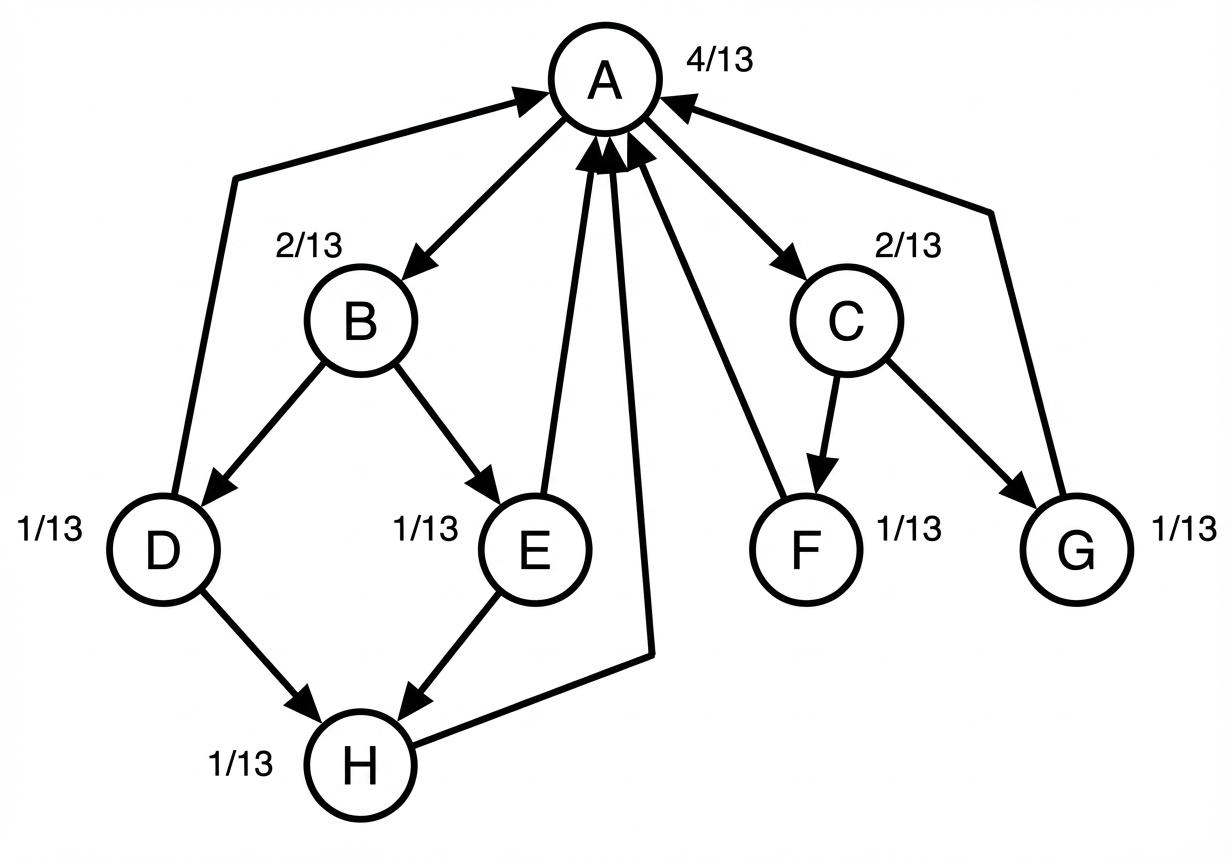
\includegraphics[width=0.6\linewidth]{images/WS_PR1.png}
    \caption{Vettore limite a partire da $f^{(0)}_i = \frac{1}{8}$}
    \label{fig:WS_PR1}
\end{figure}

Tuttavia, l'applicazione diretta di questo modello fallisce poiché il grafo del Web non è fortemente connesso. Come evidenziato nella \autoref{fig:WS_PR2}, ciò causa un accumulo irreversibile di fluido nelle componenti sconnesse (o "trappole"), dalle quali il rank non può più defluire, impedendo il raggiungimento di un equilibrio corretto.

\begin{figure}[ht!]
    \centering
    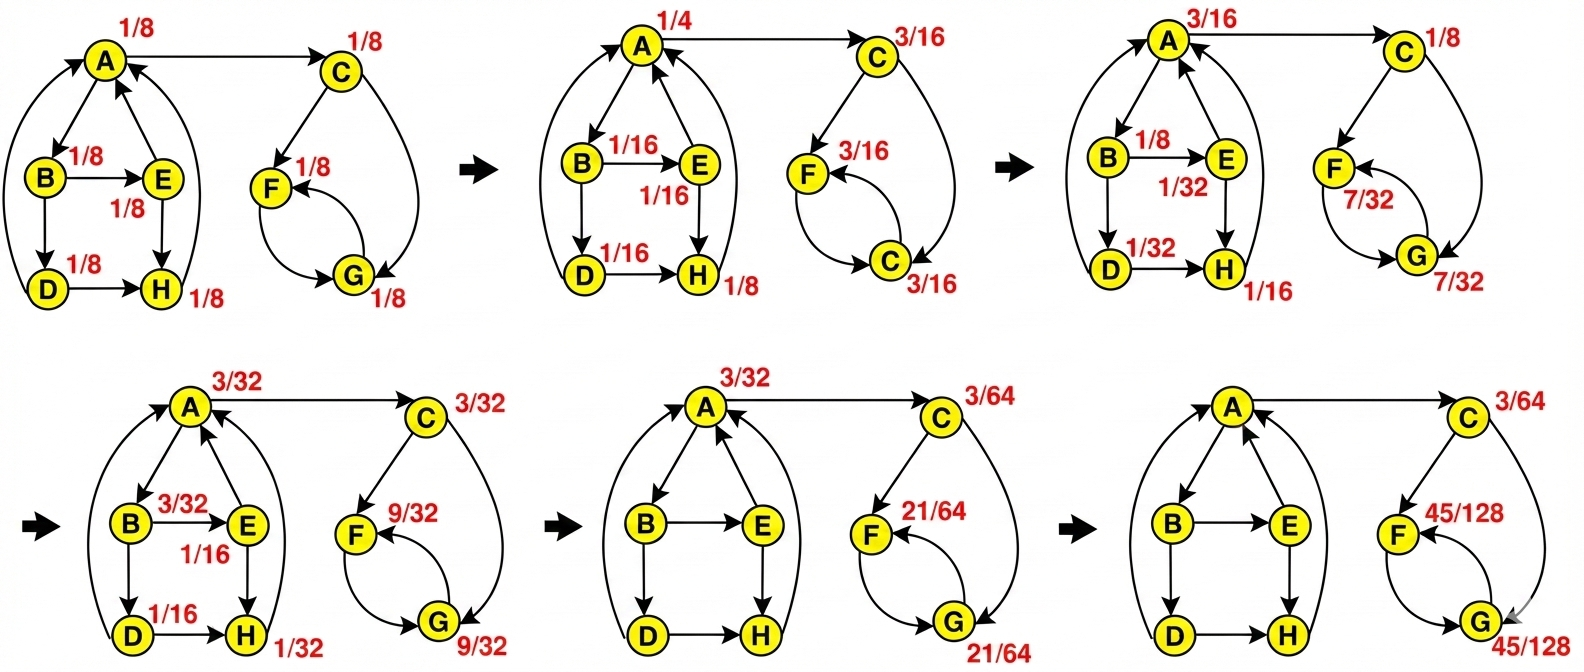
\includegraphics[width=0.8\linewidth]{images/WS_PR2.png}
    \caption{Contro esempio in cui il grafo è sconnesso}
    \label{fig:WS_PR2}
\end{figure}

\subsubsection{PageRank Scalato}

Come detto, se il grafo non è fortemente connesso (e il Web non lo è), il fluido (rank) si accumula nei nodi senza uscita e il resto della rete si svuota. er evitare questo blocco, si modifica il modo in cui il fluido viene distribuito ad ogni passo. Invece di passare tutto il rank ai vicini, se ne tiene una parte "di riserva" per ridistribuirla ovunque.

Viene introdotto un parametro $s \in [0,1]$ (chiamato solitamente \textit{damping factor}) che divide il rank di ogni nodo in due quote:

\begin{enumerate}
    \item La quota $s$: Una frazione pari a $s$ del rank del nodo viene distribuita equamente lungo gli archi uscenti (come nel PageRank classico).
    \item La quota $1 - s$: La parte rimanente, pari a $(1 - s)$, viene prelevata e distribuita uniformemente tra tutti i nodi del grafo (non solo ai vicini).
\end{enumerate}

Grazie a questa modifica, ad ogni iterazione ogni singolo nodo della rete riceve garantitamente una quantità minima di rank pari a:
\[
\frac{1 - s}{n}
\]

\begin{definizione}[Rank]
    Sia $r^{(k)}_i$ il rank posseduto dal nodo $i$ al passo $k$. Allora
    \[
    r^{(k+1)}_i = \left( \sum_{j=1: j \to i}^{n} r_j^{(k)}\frac{s}{\omega_j} \right) + \frac{1-s}{n}
    \]
\end{definizione}

Sia $N_{i,j}$ la matrice che descrive l'evoluzione del rank all'interno della rete, $\forall\ i,j = 1, \dots, n$.

\[
    N_{i,j} = 
    \begin{cases}
        \frac{s}{\omega_j} + \frac{1 - s}{n} \text{ if } j \to i \vspace{0.5 cm} \\ 
        \frac{1 - s}{n} \text{ otherwise}
    \end{cases}
\]

Infatti, sia $r^{(k)} = \left( r^{(k)}_1, r^{(k)}_2, \dots, r^{(k)}_n \right)$, l'elemento $i$-esimo di $N r^{(k)}$ è:

\begin{align*}
    \left(N r^{(k)}\right)_i = \sum_{j=1}^{n} N_{i,j} r_j^{(k)} 
    &= \sum_{j=1: j \to i}^{n} \left[ \frac{s}{\omega_j} + \frac{1 - s}{n} \right]r_j^{(k)} + \sum_{j=1: j \text{ non punta a } i}^{n} \frac{1-s}{n} r_j^{(k)} \\
    &= \sum_{j=1: j \to i}^{n} \frac{s}{\omega_j}r_j^{(k)} + \sum_{j=1}^{n} \frac{1-s}{n} r_j^{(k)} \\
    &= \sum_{j=1: j \to i}^{n} \frac{s}{\omega_j}r_j^{(k)} + \frac{1-s}{n} \underbrace{\sum_{j=1}^{n} r_j^{(k)}}_{= 1} \\
    &= \left(\sum_{j=1: j \to i}^{n} \frac{s}{\omega_j}r_j^{(k)}\right) + \frac{1-s}{n}
\end{align*}

Quindi, $r^{(k + 1)} = N r^{(k)}$. Analogamente al caso non scalato, possiamo pensare al vettore limite degli $r^{(k)}$, detto $r^*$, come ad un vettore che esprme una sorta di \textbf{configurazione di equilibrio} del rank, ossia redistribuendo il rank a partire da $r^*$, il vettore non varia: 
\[
r^* = N r^*
\]

Formalmente, il vettore limite desiderato deve corrispondere a un \textbf{autovettore stocastico} della matrice $N$, associato all'autovalore $\lambda=1$, con componenti non negative e somma pari a 1.
Il problema teorico fondamentale è dunque garantire che, per una generica matrice del Web, un tale autovettore \textbf{esista} e sia \textbf{unico}, assicurando così la stabilità del ranking.

Per dimostrare che questo autovalore esista, faremo utilizzo dei segeunti teoremi.

\begin{teorema}[Teorema di Perron]\label{teo:th_perron}
Sia $A$ una matrice reale quadrata $n \times n$ con elementi strettamente positivi. Allora valgono le seguenti proprietà:
\begin{enumerate}
    \item \textbf{Dominanza Spettrale:} La matrice $A$ possiede un autovalore reale positivo $c \in \mathbb{R}_{>0}$ che è strettamente maggiore in modulo di qualsiasi altro autovalore $\lambda$ della matrice (ovvero $c > |\lambda|$).
    \item \textbf{Autovettore Positivo e Unico:} Esiste un \textit{unico} autovettore $x$ associato a $c$ che soddisfa contemporaneamente le seguenti condizioni:
    \begin{itemize}
        \item Tutte le sue componenti sono reali e strettamente positive.
        \item La somma delle componenti è pari a 1 (normalizzazione).
    \end{itemize}
\end{enumerate}
\end{teorema}

\begin{definizione}[Matrice Stocastica]
Una matrice quadrata $A \in \mathbb{R}^{n \times n}$ si definisce \textbf{stocastica} se tutti i suoi elementi sono non negativi ($a_{ij} \ge 0$) e soddisfa una delle seguenti condizioni di normalizzazione:

\begin{itemize}
    \item \textbf{Stocastica per righe:} La somma degli elementi di ciascuna riga è uguale a 1.
    \[ \sum_{j=1}^n a_{ij} = 1 \quad \forall i \]
    \item \textbf{Stocastica per colonne:} La somma degli elementi di ciascuna colonna è uguale a 1.
    \[ \sum_{i=1}^n a_{ij} = 1 \quad \forall j \]
\end{itemize}
\end{definizione}

\begin{teorema}[Proprietà Spettrale delle Matrici Stocastiche]
Sia $A$ una matrice stocastica. Allora:

\begin{itemize}
    \item La matrice $A$ ammette sempre un autovalore $\lambda$ con modulo unitario ($|\lambda|=1$).
    \item Tale autovalore è dominante in modulo: per qualsiasi altro autovalore $\lambda'$ di $A$, vale la relazione $|\lambda'| \le 1$.
\end{itemize}
\end{teorema}

Poiché la matrice $N$ è costituita da elementi strettamente positivi, essa soddisfa pienamente le ipotesi del \autoref{teo:th_perron}.
Ciò ci garantisce che:
\begin{enumerate}
    \item Esiste un autovalore dominante $c$ reale e positivo.
    \item A tale autovalore corrisponde un autovettore $x$ \textbf{unico}, avente componenti tutte reali e positive, la cui somma è normalizzata a 1.
\end{enumerate}

Inoltre, dimostriamo che $N$ è una matrice \textbf{stocastica per colonne}. Infatti, sommando gli elementi di una generica colonna $j$, abbiamo che per ogni riga $i$:

\begin{proof}
    Poiché
    \[
        \sum_{i=1: j \to i}^{n} \frac{1}{\omega_j} = 1
    \]
    allora,
    \begin{align*}
        \sum_{i=1}^{n} N_{i,j} 
        &= \sum_{i=1: j \to i}^{n} \left[ \frac{s}{\omega_j} + \frac{1 - s}{n} \right] + \sum_{i=1: j \text{ non punta a } i}^{n} \frac{1-s}{n}\\
        &= \sum_{i=1: j \to i}^{n} \frac{s}{\omega_j} + \sum_{i=1}^{n} \frac{1-s}{n} = s + n \frac{1-s}{n} = 1
    \end{align*}
\end{proof}

\textbf{In conclusione}, $r^* = N r^*$.

\subsection{PageRank e RandomWalk}

Oltre all'interpretazione basata sul "fluido", il PageRank possiede una lettura probabilistica legata al concetto di \textit{random walk} (passeggiata aleatoria) su un grafo diretto $G = (V, A)$.

Immaginiamo un navigatore che si muove nella rete seguendo queste regole:
\begin{enumerate}
    \item \textbf{Inizializzazione:} Sceglie uniformemente a caso un nodo iniziale $u \in V$.
    \item \textbf{Navigazione:} Da $u$, sceglie uniformemente a caso un arco uscente che conduce a un nuovo nodo.
    \item \textbf{Iterazione:} Ripete il processo dal nuovo nodo, generando un percorso aleatorio infinito.
\end{enumerate}

Per analizzare la relazione tra questo processo e il PageRank, definiamo per ogni nodo $i \in V$ la variabile aleatoria $w_i^k$:
\[
w_i^k = 
\begin{cases} 
1 & \text{se al passo } k \text{ del random walk ci troviamo nel nodo } i \\
0 & \text{altrimenti}
\end{cases}
\]

Indichiamo con $f_i^{(k)}$ la probabilità di trovarsi nel nodo $i$ al passo $k$:
\[ f_i^{(k)} = \Pr\left[w_i^k = 1\right] \]

Il calcolo delle probabilità avviene induttivamente:

\begin{itemize}
    \item \textbf{Passo Base ($k=0$):} Poiché il nodo iniziale è scelto uniformemente tra gli $n$ nodi del grafo, la probabilità iniziale è:
    \[
    f_i^{(0)} = \Pr \left[w_i^0 = 1\right] = \frac{1}{n}
    \]
    
    \item \textbf{Passo Induttivo ($k > 0$):} Sia $\omega_j$ il numero di archi uscenti dal nodo $j$ (grado uscente). La probabilità di trovarsi in $i$ al passo $k$ dipende dalla probabilità di trovarsi in un nodo $j$ che punta a $i$ al passo precedente ($k-1$), moltiplicata per la probabilità di transizione $1/\omega_j$:
    \[
    f_i^{(k)} = \Pr\left[w_i^k = 1\right] = \sum_{j \in V : (j,i) \in A} \frac{1}{\omega_j} \Pr\left[w_j^{k-1} = 1\right] = \sum_{j \in V : (j,i) \in A} \frac{f_j^{(k-1)}}{\omega_j}
    \]
\end{itemize}

Nel modello scalato, introduciamo un parametro $s \in [0,1]$. Ad ogni passo il navigatore:
\begin{itemize}
    \item Con probabilità $s$ segue un arco uscente.
    \item Con probabilità $(1-s)$ salta uniformemente verso un qualsiasi nodo del grafo (teletrasporto).
\end{itemize}

Indichiamo con $sw_i^k$ la variabile aleatoria nel modello scalato. La relazione di ricorrenza diventa:

\[
\Pr\left[sw_i^k = 1\right] = \underbrace{\sum_{j \in V: (j,i) \in A} \frac{s}{\omega_j} \Pr\left[sw_j^{k-1} = 1\right]}_{\text{Navigazione Link}} + \underbrace{\frac{1-s}{n}}_{\text{Teletrasporto}} = r_i^{(k)}
\]

In questa ottica, il PageRank di una pagina rappresenta la probabilità stazionaria che un "navigatore casuale" si trovi su quella pagina dopo un numero sufficientemente grande di passi.

\end{document}
